\documentclass[10pt]{article}
\usepackage[utf8]{inputenc}
\usepackage{amsmath} 
\usepackage{color} %For interrogation about report or code
\usepackage[table]{xcolor}
\usepackage{graphicx} %To include image
\usepackage{supertabular}

\usepackage{hyperref} %Liens hypertexte du sommaire

\usepackage[english]{}

\DeclareGraphicsExtensions{.pdf,.png,.jpg} %

\usepackage[dvips]{geometry} % TO MODIFY THE MARGE
\geometry{
	right = 2cm,
	top=1.5cm,
}

\title{Trampoline (OSEK/VDX OS) Test Plan - Version 1.0}
\author{Florent PAVIN}

% INITIALISATION %
%% HEAD SUPERTABULAR %%
\newlength{\Li}\settowidth{\Li}{Case}
\newlength{\Lii}\setlength{\Lii}{7cm}
\newlength{\Liii}\setlength{\Liii}{\textwidth} \addtolength{\Liii}{-\Li} \addtolength{\Liii}{-\Lii}
\newlength{\Liiii}\setlength{\Liiii}{\textwidth} \addtolength{\Liiii}{-\Li}

\tablefirsthead{ \hline \rowcolor{lightgray} Test Case No. & Action & Expected Result  \\ }
\tablehead{ \hline \rowcolor{lightgray} Test Case No. & Action & Expected Result \\ }
\tabletail{ \hline} 
\tablelasttail{}

% BEGIN DOCUMENT %
\begin{document}

% MISE EN PAGE %
%\setlength{\hoffset}{10pt}

\maketitle
\tableofcontents

\section{Introduction}
This document contains the test plan for the conformance test of the operating system. This means definition of the test cases, which are used to certify conformance of an OS implementation. For more information about what is a test plan and his link to the conformance methodology previously defined, see OSEK Test Plan 2.0  \cite{OSEK_Test_Plan_20}.\\
Unlike OSEK Test Plan 2.0  which is based from OSEK OS 2.0  \cite{OSEK_OS_20}, this test plan is defined from OSEK OS 2.2.3  \cite{OSEK_OS_223} and the internal communication of OSEK Communication 3.0.3 \cite{OSEK_COM_303} .\\

\section{Test cases}
This chapter contains the test cases which will be used to test an implementation of an operating system to be OSEK conform. Thus, they are developed on the basis of the OSEK OS specification, according to figure 12-1 API service restrictions from OSEK/VDX OS v2.2.3. The internal communication comes from CCCB conformance class (\cite{OSEK_COM_303} p.59).\\
As we said earlier, this test plan is defined from the OSEK OS version 2.2.3, and to better see the differences between this version and the old one (OSEK Test Plan 2.0), we will explain those differences in each section.\\
ISR1 does not use an operating system service since after the ISR1 is finished, processing continues exactly at the instruction where the interrupt has occurred, i.e. the interrupt has no influence on task management. Thus, \textbf{ISR can't be tested}.\\
\textit{Stack Monitoring}, from AUTOSAR OS, is not a functional test. It has to be tested in every target because it's depending on the portage. \textit{Stack Monitoring} OS Requirements (OS067, OS068, OS396) are therfore not included in this report.\\
Idem for \textit{Protecting the Hardware}.\\
	
Meanwhile, \textit{Memory Protection} OS Requirements (OS026, OS027, OS044, OS081, OS083, OS086, OS087, OS195, OS196, OS198, OS207, OS208, OS209, OS355, OS356) are tested (see  \ref{memprot}).\\

	%TASK MANAGEMENT %
	\subsection{Task management}
	Since Schedule() returns E\_OS\_RESSOURCE from a task or an interrupt when a resource is occupied, test case 33 appears.\\
	Since GetTaskID returns E\_OK from an interrupt, test case 35 appears.\\
	Category 3 interrupts have been removed. \\

	\begin{figure}[htbp] %  figure placement: here, top, bottom, or page
   		\centering
		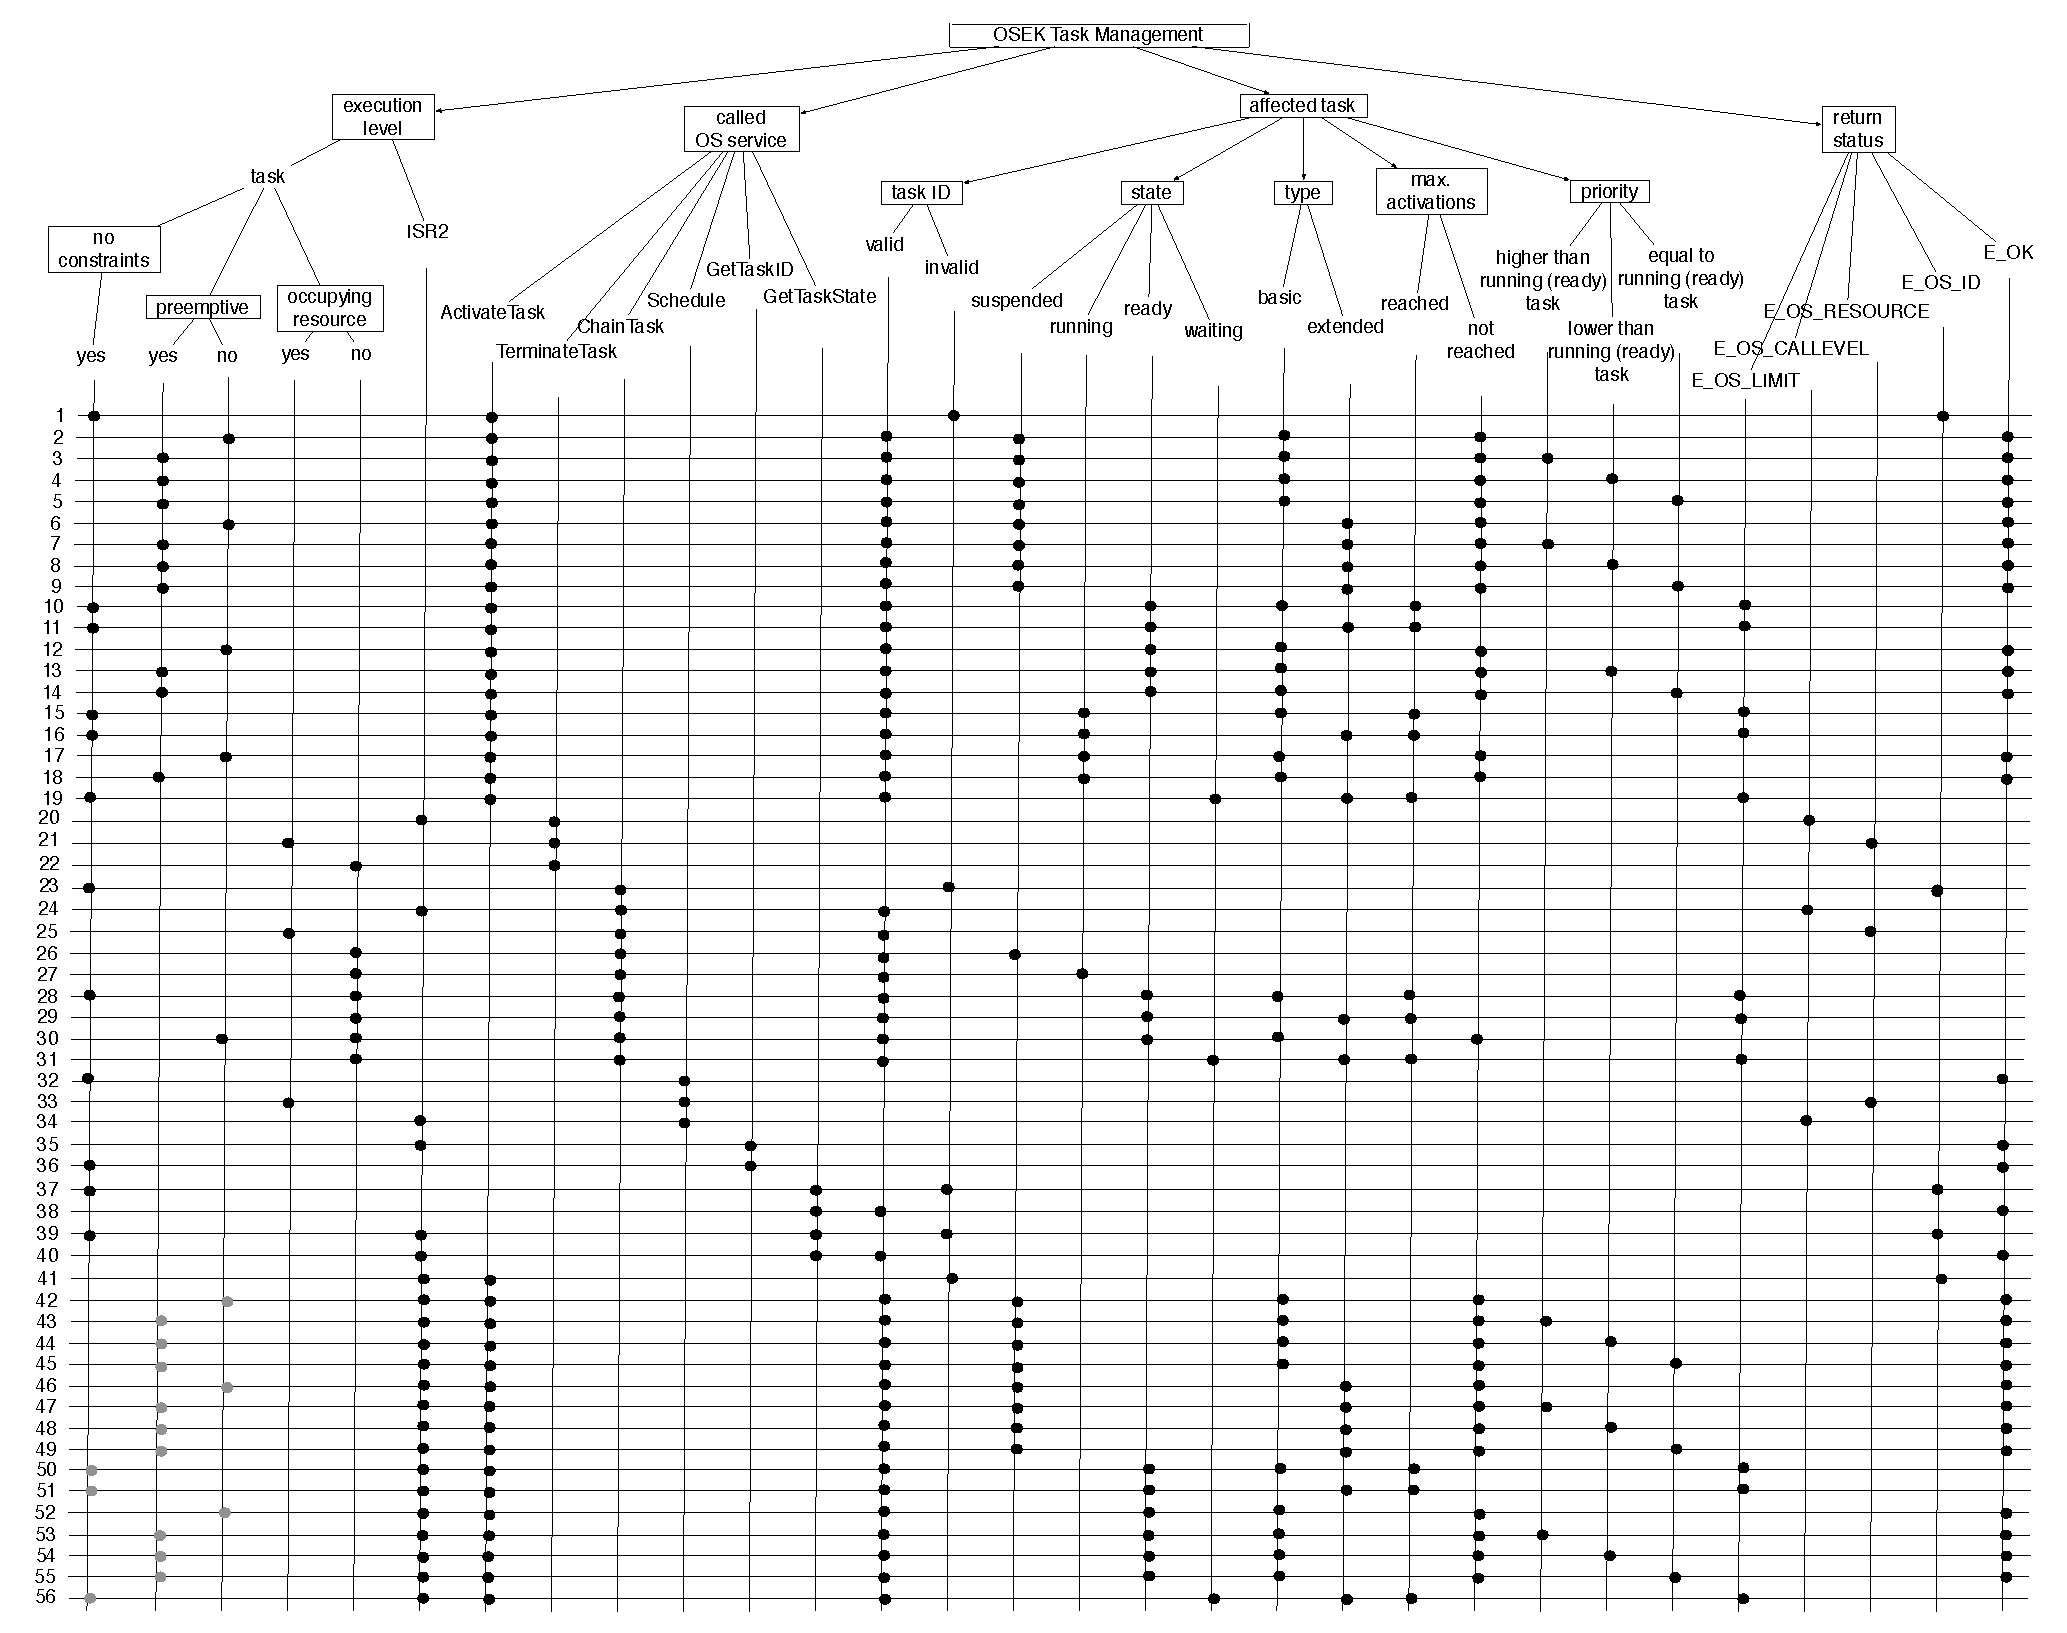
\includegraphics[width=1\textheight, angle=90]{graphics/OSEK_Task_Management.pdf}
	\end{figure}		
	
	\begin{supertabular}{|p{\Li}|p{\Lii}|p{\Liii}|} \hline
	1	& Call ActivateTask() from task-level with invalid task ID (task does not exist) 			& Service returns E\_OS\_ID  \\ \hline
	2	& Call ActivateTask() from non-preemptive task on suspended basic task 			& No preemption of running task. Activated task becomes ready. Service returns E\_OK  \\ \hline
	3	& Call ActivateTask() from preemptive task on suspended basic task which has higher priority than running task. & Running task is preempted. Activated task becomes running. Service returns E\_OK  \\ \hline
	4	& Call ActivateTask() from preemptive task on suspended basic task which has lower priority than running task. & No preemption of running task. Activated task becomes ready. Service returns E\_OK \\ \hline
	5 	& Call ActivateTask() from preemptive task on suspended basic task which has equal priority as running task. & No preemption of running task. Activated task becomes ready. Service returns E\_OK  \\ \hline
	6 	& Call ActivateTask() from non-preemptive task on suspended extended task 			& No preemption of running task. Activated task becomes ready and its 
events are cleared. Service returns E\_OK  \\ \hline
	7 	& Call ActivateTask() from preemptive task on suspended extended task which has higher priority than running task. & Running task is preempted. Activated task becomes running and its events are cleared. Service returns E\_OK  \\ \hline
	8 	& Call ActivateTask() from preemptive task on suspended extended task which has lower priority than running task. & No preemption of running task. Activated task becomes ready and its events are cleared. Service returns E\_OK  \\ \hline
	9	& Call ActivateTask() from preemptive task on suspended extended task which has equal priority as running task. & No preemption of running task. Activated task becomes ready and its events are cleared. Service returns E\_OK  \\ \hline
	10 	& Call ActivateTask() on ready basic task which has reached max. number of activations & Service returns E\_OS\_LIMIT  \\ \hline
	11	& Call ActivateTask() on ready extended task 									& Service returns E\_OS\_LIMIT  \\ \hline
	12 	& Call ActivateTask() from non-preemptive task on ready basic task which has not reached max. number of activations & No preemption of running task. Activation request is queued in ready list. Service returns E\_OK  \\ \hline
	13 	& Call ActivateTask() from preemptive task on ready basic task which has not reached max. number of activations and has lower priority than running task1 & No preemption of running task. Activation request is queued in ready list. Service returns E\_OK  \\ \hline
	14	& Call ActivateTask() from preemptive task on ready basic task which has not reached max. number of activations and has equal priority as running task & No preemption of running task. Activation request is queued in ready list. Service returns E\_OK  \\ \hline
	15 	& Call ActivateTask() on running basic task which has reached max. number of activations & Service returns E\_OS\_LIMIT  \\ \hline
	16	& Call ActivateTask() on running extended task								& Service returns E\_OS\_LIMIT  \\ \hline
	17	& Call ActivateTask() from non-preemptive task on running basic task which has not reached max. number of activations & No preemption of running task. Activation request is queued in ready list. Service returns E\_OK  \\ \hline
	18	& Call ActivateTask() from preemptive task on running basic task which has not reached max. number of activations & No preemption of running task. Activation request is queued in ready list. Service returns E\_OK  \\ \hline
	19	& Call ActivateTask() on waiting extended task 								& Service returns E\_OS\_LIMIT  \\ \hline
	20	& Call TerminateTask() from ISR category 2 									& Service returns E\_OS\_CALLEVEL  \\ \hline
	21 	& Call TerminateTask() while still occupying a resource Running task is not terminated. 	& Service returns E\_OS\_RESOURCE  \\ \hline
	22	& Call TerminateTask() 													& Running task is terminated and ready task with highest priority is executed \\ \hline
	23	& Call ChainTask() from task-level. Task-ID is invalid (does not exist). 				& Service returns E\_OS\_ID  \\ \hline
	24	& Call ChainTask() from ISR category 2 										& Service returns E\_OS\_CALLEVEL  \\ \hline
	25	& Call ChainTask() while still occupying a resource 								& Running task is not terminated. Service returns E\_OS\_RESOURCE  \\ \hline
	26	& Call ChainTask() on suspended task 										& Running task is terminated, chained task becomes ready and ready task 
with highest priority is executed \\ \hline
	27 	& Call ChainTask() on running task 											& Running task is terminated, chained task becomes ready and ready task with highest priority is executed \\ \hline
	28	& Call ChainTask() on ready basic task which has reached max. number of activations 	& Running task is not terminated. Service returns E\_OS\_LIMIT  \\ \hline
	29	& Call ChainTask() on ready extended task 									& Running task is not terminated. Service returns E\_OS\_LIMIT  \\ \hline
	30 	& Call ChainTask() from non-preemptive task on ready basic task which has not reached max. number of activations & Running task is terminated, activation request is queued in ready list and ready task with highest priority is executed  \\ \hline
	31	& Call ChainTask() on waiting extended task 									& Service returns E\_OS\_LIMIT  \\ \hline
	32 	& Call Schedule() from task. 												& Ready task with highest priority is executed. Service returns E\_OK  \\ \hline
	33	& Call Schedule() while still occupying a resource								& Service returns E\_OS\_RESOURCE  \\ \hline
	34 	& Call Schedule() from ISR category 2 										& Service returns E\_OS\_CALLEVEL \\ \hline
	35 	& Call GetTaskID() from ISR category 2 										& Service returns  E\_OK  \\ \hline
	36	& Call GetTaskID() from task 												& Return task ID of currently running task. Service returns E\_OK \\ \hline
	37	& Call GetTaskState() with invalid task ID (task does not exist) 						& Service returns E\_OS\_ID \\ \hline
	38	& Call GetTaskState() Return state of queried task.								& Service returns E\_OK  \\ \hline
	
	39	& Call GetTaskState() from ISR2 with invalid task ID (task does not exist)				& Service returns E\_OS\_ID \\ \hline
	40	& Call GetTaskState() from ISR2. Return state of queried task.						& Service returns E\_OK  \\ \hline
	
	41	& Call ActivateTask() from ISR2 with invalid task ID (task does not exist)				& Service returns E\_OS\_ID  \\ \hline
	42	& Call ActivateTask() from ISR2 (in non-preemptive mode) on suspended basic task.		& Activated task becomes ready. Service returns E\_OK  \\ \hline
	43	& Call ActivateTask() from ISR2 (in preemptive mode) on suspended basic task which has higher priority than last running task. & Activated task becomes ready and first. Service returns E\_OK  \\ \hline
	44	& Call ActivateTask() from ISR2 (in preemptive mode) on suspended basic task which has lower priority than last running task. & Activated task becomes ready. Service returns E\_OK \\ \hline
	45 	& Call ActivateTask() from ISR2 (in preemptive mode) on suspended basic task which has equal priority as last running task. & Activated task becomes ready. Service returns E\_OK  \\ \hline
	46 	& Call ActivateTask() from ISR2 (in non-preemptive mode) on suspended extended task 	& Activated task becomes ready and its 
events are cleared. Service returns E\_OK  \\ \hline
	47 	& Call ActivateTask() from ISR2 (in preemptive mode) on suspended extended task which has higher priority than last running task. & Activated task becomes ready and first and its events are cleared. Service returns E\_OK  \\ \hline
	48 	& Call ActivateTask() from ISR2 (in preemptive mode) on suspended extended task which has lower priority than last running task. & Activated task becomes ready and its events are cleared. Service returns E\_OK  \\ \hline
	49	& Call ActivateTask() from ISR2 (in preemptive mode) on suspended extended task which has equal priority as last running task. & Activated task becomes ready and its events are cleared. Service returns E\_OK  \\ \hline
	50 	& Call ActivateTask() from ISR2 on ready basic task which has reached max. number of activations & Service returns E\_OS\_LIMIT  \\ \hline
	51	& Call ActivateTask() from ISR2 on ready extended task 									& Service returns E\_OS\_LIMIT  \\ \hline
	52 	& Call ActivateTask() from ISR2 (in non-preemptive mode) on ready basic task which has not reached max. number of activations & Activation request is queued in ready list. Service returns E\_OK  \\ \hline
	53 	& Call ActivateTask() from ISR2 (in preemptive mode) on ready basic task which has not reached max. number of activations and has higher priority than last running & Activation request is queued in ready list on first place. Service returns E\_OK  \\ \hline
	54 	& Call ActivateTask() from ISR2 (in preemptive mode) on ready basic task which has not reached max. number of activations and has lower priority than last running task1 & Activation request is queued in ready list. Service returns E\_OK  \\ \hline
	55	& Call ActivateTask() from ISR2 (in preemptive mode) on ready basic task which has not reached max. number of activations and has equal priority as last running task & Activation request is queued in ready list. Service returns E\_OK  \\ \hline
	56	& Call ActivateTask() from ISR2 on waiting extended task 								& Service returns E\_OS\_LIMIT  \\ \hline
	
	\end{supertabular} \\  
	
	%INTERRUPT PROCESING %
	\subsection{Interrupt processing}
	New routines appear (EnableAllInterrupts, DisableAllInterrupts, SuspendAllInterrupts, ResumeAllInterrupts, SuspendOSInterrupts, ResumeOSInterrupts), test cases 1 to 19 are new ones. \\
	Category 3 interrupts have been removed. \\
	Maximum number of activation of ISR2 can't be more than 1.\\
	EnableAllInterrupts, ResumeAllInterrupts and ResumeOSInterrupts from ISR2 are only tested with an interrupt trigged with a priority higher than running ISR2.\\ 
	SuspendAllInterrupts and ResumeAllInterrupts are the only ones functions allowed in callback routines.\\
		
	\begin{figure}[htbp] %  figure placement: here, top, bottom, or page
   		\centering
		\includegraphics[width=1\textheight, angle=90]{graphics/OSEK_Interrupt_processing.pdf}
	\end{figure}	
	
	\begin{supertabular}{|p{\Li}|p{\Lii}|p{\Liii}|} \hline
	1	& Call EnableAllInterrupts() from task. An interrupt has been trigged in disable mode	& The Interrupt is executed. Running task become ready \\ \hline
	2	& Call EnableAllInterrupts() from task										& Enable all interrupts \\ \hline
	3	& Call EnableAllInterrupts() from task without calling DisableAllInterrupts()			& The service is not performed \\ \hline
	4	& Call DisableAllInterrupts() from task										& Disable all interrupts \\ \hline
	
	5	& Call ResumeAllInterrupts() from task. An interrupt has been trigged in disable mode	& The Interrupt is executed. Running task become ready \\ \hline
	6	& Call ResumeAllInterrupts() from task										& Resume all interrupts \\ \hline
	7	& Call ResumeAllInterrupts() from task as many times as SuspendAllInterrupts() is previously called	& Resume all interrupts \\ \hline
	8	& Call ResumeAllInterrupts() from task without calling SuspendAllInterrupts()			& The service is not performed \\ \hline
	9	& Call SuspendAllInterrupts() from task										& Suspend all interrupts \\ \hline
	
	10	& Call ResumeOSInterrupts() from task. An interrupt has been trigged in disable mode	& The Interrupt is executed. Running task become ready \\ \hline
	11	& Call ResumeOSInterrupts() from task										& Resume OS interrupts \\ \hline	
	12	& Call ResumeOSInterrupts() from task as many times as SuspendOSInterrupts() is previously called	& Resume OS interrupts \\ \hline
	13	& Call ResumeOSInterrupts() from task without calling SuspendOSInterrupts()			& The service is not performed \\ \hline
	14	& Call SuspendOSInterrupts() from task										& Suspend OS interrupts \\ \hline
	
	15	& Interruption of running task  												& Interrupt is executed \\ \hline
	16	& Interruption of running task with the same interrupt already trigged (activation count = activation max)		& Interrupt is discarded \\ \hline
	17	& Return from ISR2. Interrupted task is non-preemptive							& Execution of interrupted task is continued \\ \hline
	18	& Return from ISR2. Interrupted task is preemptive								& Ready task with highest priority is executed (Rescheduling) \\ \hline
	19	& Call any OS service between Suspend/Disable- and Resume/Enable- pairs			& Service returns E\_OS\_DISABLEINT and not perform the service (see AUTOSAR OS092), even Disable and Enable pairs (see OSEK p26) \\ \hline
	
	20	& Call EnableAllInterrupts() from ISR2. An interrupt has been trigged in disable mode with a higher priority than running ISR2	& The Interrupt is executed. Running ISR2 becomes ready \\ \hline
	21	& Call EnableAllInterrupts() from ISR2										& Enable all interrupts \\ \hline
	22	& Call DisableAllInterrupts() from ISR2										& Disable all interrupts \\ \hline
	23	& Call ResumeAllInterrupts() from ISR2. An interrupt has been trigged in disable mode with a higher priority than running ISR2	& The Interrupt is executed. Running ISR2 becomes ready \\ \hline
	24	& Call ResumeAllInterrupts() from ISR2										& Resume all interrupts \\ \hline
	25	& Call ResumeAllInterrupts() from ISR2 as many times as SuspendAllInterrupts() is previously called	& Resume all interrupts \\ \hline
	26	& Call SuspendAllInterrupts() from ISR2										& Suspend all interrupts \\ \hline
	27	& Call ResumeOSInterrupts() from ISR2. An interrupt has been trigged in disable mode with a higher priority than running ISR2	& The Interrupt is executed. Running ISR2 becomes ready \\ \hline
	28	& Call ResumeOSInterrupts() from ISR2										& Resume OS interrupts \\ \hline	
	29	& Call ResumeOSInterrupts() from ISR2 as many times as SuspendOSInterrupts() is previously called	& Resume OS interrupts \\ \hline
	30	& Call SuspendOSInterrupts() from ISR2									& Suspend OS interrupts \\ \hline
	31	& Interruption of running ISR2 on interrupt which has higher priority than running interrupt & Running Interrupt is preempted. Executed interrupt becomes running \\ \hline
	32	& Interruption of running ISR2	on interrupt which has lower priority than running interrupt & No preemption of running interrupt. Executed interrupt becomes ready \\ \hline
	33	& Interruption of running ISR2	on interrupt which has equal priority as running interrupt & No preemption of running interrupt. Executed interrupt becomes ready \\ \hline
	34	& Return from ISR2 to an ISR2 which has higher priority than ISR2 preempted			& ISR2 with the highest priority is executed \\ \hline
	35	& Call ResumeAllInterrupts() from callback routine. An interrupt has been trigged in disable mode		& No preemption of callback routine because ISR2 are disabled in callback routines \\ \hline
	36	& Call ResumeAllInterrupts() from callback routine								& Resume all interrupts \\ \hline
	37	& Call ResumeAllInterrupts() from callback routine as many times as SuspendAllInterrupts() is previously called	& Resume all interrupts \\ \hline
	38	& Call SuspendAllInterrupts() from callback routine								& Suspend all interrupts \\ \hline
	39	& Interruption in callback routines											& Interrupt is executed after callback routines \\ \hline
	
	
	\end{supertabular} \\  
	
	% EVENT MECHANISM %
	\subsection{Event mechanism}
	Category 3 interrupts have been removed. \\
	Test cases 9 and 10 have to be tested with a simple ready task and with a READY\_AND\_NEW task (a task which juste came to be ready).\\
	Test cases 41 to 43 are GOIL test cases. \\
	
	\begin{figure}[htbp] %  figure placement: here, top, bottom, or page
   		\centering
		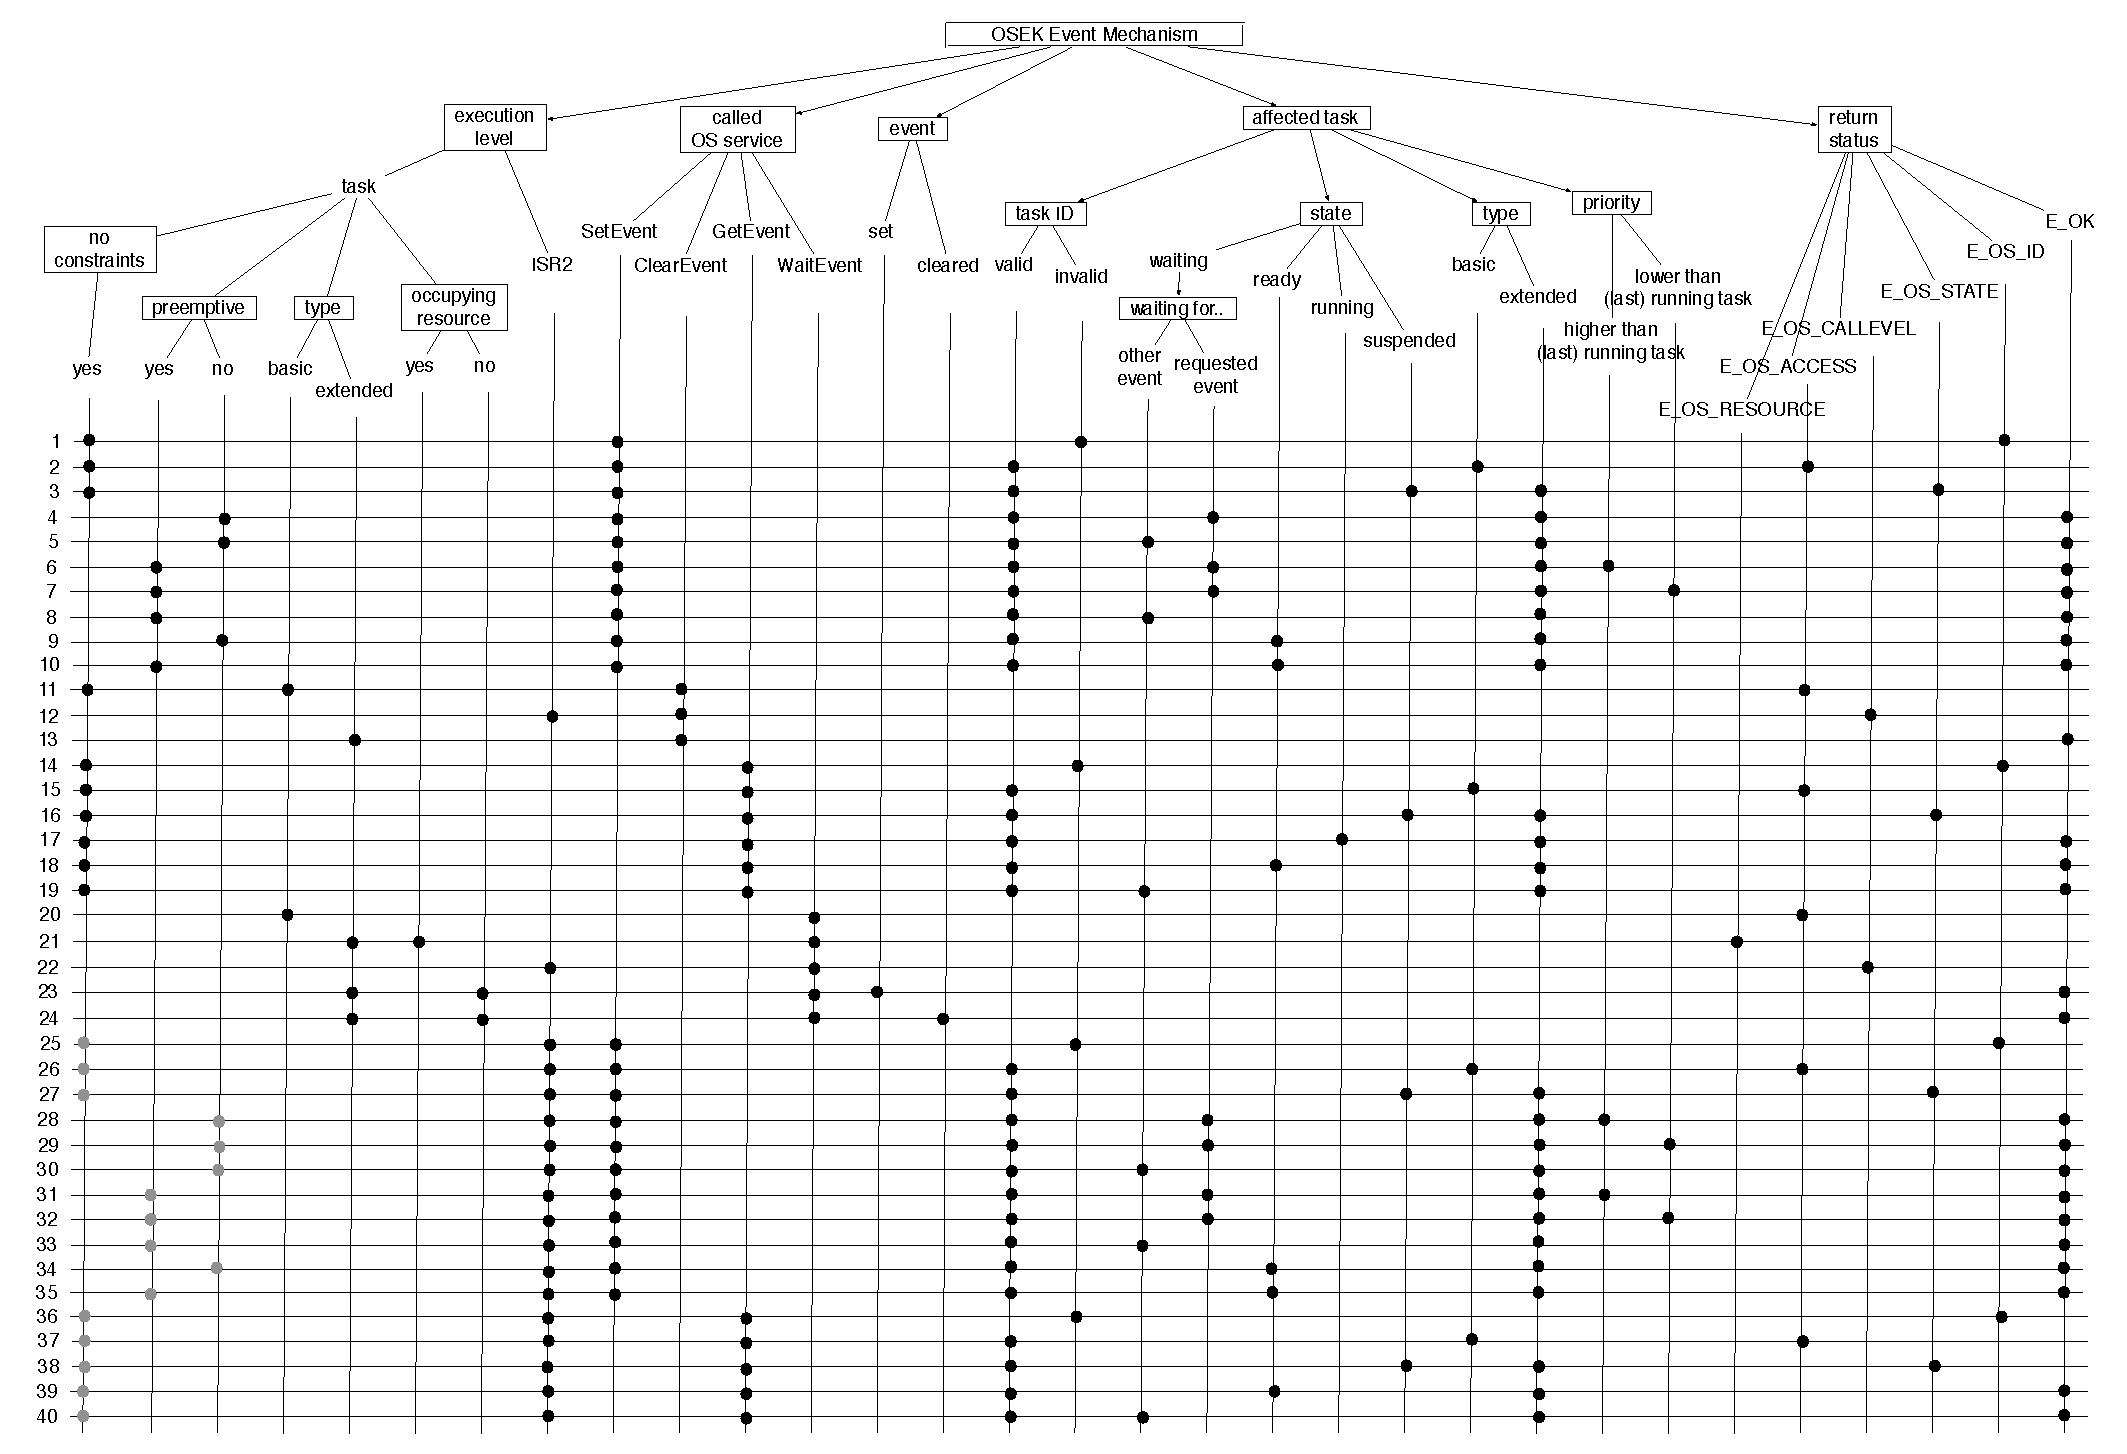
\includegraphics[width=1\textheight, angle=90]{graphics/OSEK_Event_Mechanism.pdf}
	\end{figure}
	
	\begin{supertabular}{|p{\Li}|p{\Lii}|p{\Liii}|} \hline
	1	& Call SetEvent() with invalid Task ID										& Service returns E\_OS\_ID  \\ \hline
	2	& Call SetEvent() for basic task 											& Service returns E\_OS\_ACCESS  \\ \hline
	3	& Call SetEvent() for suspended extended task 								& Service returns E\_OS\_STATE \\ \hline
	4	& Call SetEvent() from non-preemptive task on waiting extended task which is waiting for at least one of the requested events
																			& Requested events are set. Running task is not preempted. Wainting task becomes ready. Service returns E\_OK  \\ \hline
	5 	& Call SetEvent() from non-preemptive task on waiting extended task which is not waiting for any of the requested events
																			& Requested events are set. Running task is not preempted. Waiting task doesn’t become ready. Service returns E\_OK  \\ \hline
	6	& Call SetEvent() from preemptive task on waiting extended task which is waiting for at least one of the requested events and has higher priority than running task
																			& Requested events are set. Running task becomes ready (is preempted). Waiting task becomes running. Service returns E\_OK  \\ \hline
	7 	& Call SetEvent() from preemptive task on waiting extended task which is waiting for at least one of the requested events and has equal or lower priority than running task																			& Requested events are set. Running  task is not preempted. Waiting task becomes ready. Service returns E\_OK \\ \hline
	8 	& Call SetEvent() from  preemptive task on waiting extended task which is not waiting for any of the requested events
																			& Requested events are set. Running task is not preempted. Waiting task doesn’t become ready. Service returns E\_OK  \\ \hline
	9	& Call SetEvent() from non-preemptive task on ready extended task 				& Requested events are set. Running task is not preempted. Service returns E\_OK \\ \hline
	10	& Call SetEvent() from preemptive task on ready extended task 					& Requested events are set. Running task is not preempted. Service returns E\_OK \\ \hline
	11	& Call ClearEvent() from basic task											& Service returns E\_OS\_ACCESS  \\ \hline
	12	& Call ClearEvent() from ISR2 												& Service returns E\_OS\_CALLEVEL \\ \hline
	13 	& Call ClearEvent() from extended task 										& Requested events are cleared. Service returns E\_OK  \\ \hline
	14	& Call GetEvent() with invalid Task ID 										& Service returns E\_OS\_ID  \\ \hline
	15 	& Call GetEvent() for basic task 											& Service returns E\_OS\_ACCESS \\ \hline
	16	& Call GetEvent() for suspended extended task 								& Service returns E\_OS\_STATE  \\ \hline
	17	& Call GetEvent() for running extended task									& Return current state of all event bits. Service returns E\_OK  \\ \hline
	18	& Call GetEvent() for ready extended task 									& Return current state of all event bits. Service returns E\_OK  \\ \hline
	19	& Call GetEvent() for waiting extended task 									& Return current state of all event bits. Service returns E\_OK  \\ \hline
	20 	& Call WaitEvent() from basic task											& Service returns E\_OS\_ACCESS  \\ \hline
	21 	& Call WaitEvent() from extended task which occupies a resource 					& Service returns E\_OS\_RESOURCE  \\ \hline
	22 	& Call WaitEvent() from ISR2												& Service returns E\_OS\_CALLEVEL \\ \hline
	23	& Call WaitEvent() from extended task. None of the events waited for is set 			& Running task becomes waiting and ready task with highest priority is executed Service returns E\_OK  \\ \hline
	24	& Call WaitEvent() from extended task. At least one event waited for is already set 		& No preemption of running task Service returns E\_OK \\ \hline
	
	25	& Call SetEvent() from ISR2 with invalid Task ID								& Service returns E\_OS\_ID  \\ \hline
	26	& Call SetEvent() from ISR2 for basic task 									& Service returns E\_OS\_ACCESS  \\ \hline
	27	& Call SetEvent() from ISR2 for suspended extended task 						& Service returns E\_OS\_STATE \\ \hline
	28	& Call SetEvent() from ISR2 (in non-preemptive mode) on waiting extended task which is waiting for at least one of the requested events and has higher priority than last running task																& Requested events are set. Waiting task becomes ready. Service returns E\_OK  \\ \hline
	29	& Call SetEvent() from ISR2 (in non-preemptive mode) on waiting extended task which is waiting for at least one of the requested events and has lower priority than last running task																& Requested events are set. Waiting task becomes ready. Service returns E\_OK  \\ \hline
	30 	& Call SetEvent() from ISR2 (in non-preemptive mode) on waiting extended task which is not waiting for any of the requested events
																			& Requested events are set. Waiting task doesn’t become ready. Service returns E\_OK  \\ \hline
	31	& Call SetEvent() from ISR2 (in preemptive mode) on waiting extended task which is waiting for at least one of the requested events and has higher priority than running task																	& Requested events are set. Waiting task becomes ready and first. Service returns E\_OK  \\ \hline
	32	& Call SetEvent() from ISR2 (in preemptive mode) on waiting extended task which is waiting for at least one of the requested events and has equal or lower priority than running task																			& Requested events are set. Waiting task becomes ready. Service returns E\_OK \\ \hline
	33	& Call SetEvent() from ISR2 (in preemptive mode) on waiting extended task which is not waiting for any of the requested events
																			& Requested events are set. Waiting task doesn’t become ready. Service returns E\_OK  \\ \hline
	34	& Call SetEvent() from ISR2 (in non-preemptive mode) on ready extended task 		& Requested events are set. Service returns E\_OK \\ \hline
	35	& Call SetEvent() from ISR2 (in preemptive mode) on ready extended task 			& Requested events are set. Service returns E\_OK \\ \hline
	36	& Call GetEvent() from ISR2 with invalid Task ID 								& Service returns E\_OS\_ID  \\ \hline
	37 	& Call GetEvent() from ISR2 for basic task 									& Service returns E\_OS\_ACCESS \\ \hline
	38	& Call GetEvent() from ISR2 for suspended extended task 						& Service returns E\_OS\_STATE  \\ \hline
	39	& Call GetEvent() from ISR2 for ready extended task 							& Return current state of all event bits. Service returns E\_OK  \\ \hline
	40	& Call GetEvent() from ISR2 for waiting extended task 							& Return current state of all event bits. Service returns E\_OK  \\ \hline
	
	41	& Creating an event with a MASK using more than one bit						& Warning : Event Mask uses more than one bit \\ \hline
	42	& Creating an event with a MASK already used								& Error : Mask already used \\ \hline
	43	& Creating an event with an automatic MASK but all the MASK are already used		& Error : All mask bits are already used, the last event can't be created \\ \hline
	\end{supertabular} \\
	
	% RESOURCE MANAGEMENT %
	\subsection{Resource management}
	An ISR2 is like a task, it can get and release resources if it's allowed (if it owns the resource). See test cases 3, 4, 9 and 10.\\
	GetResource() returns E\_OS\_ACCESS if the resource's priority is inferior to the task's priority (it means the task doesn't use it so if it gets the resource, the resource is not well shared). Otherwise, a task is allowed to get a Resource with a priority higher than itself. \\
	There's no more maximum number of nested resources reachable. \\
	Category 3 interrupts have been removed. \\

	\begin{figure}[htbp] %  figure placement: here, top, bottom, or page
   		\centering
		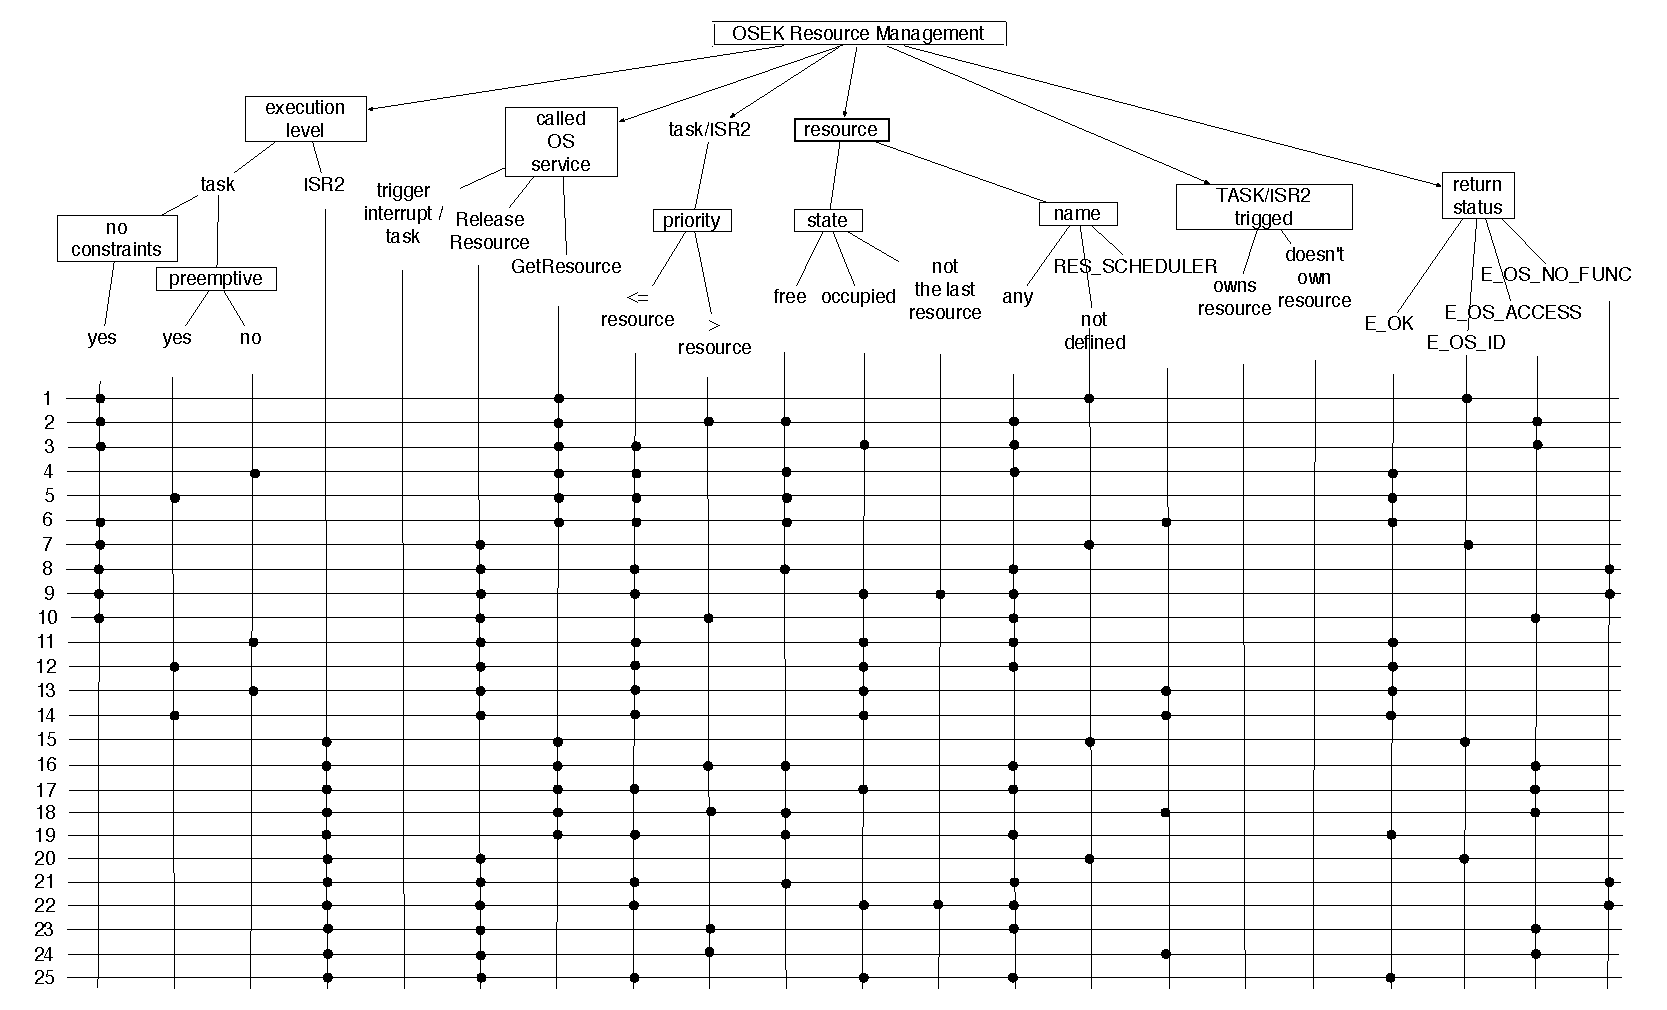
\includegraphics[width=1\textwidth]{graphics/OSEK_Resource_Management.pdf}
	\end{figure}
		
	\begin{supertabular}{|p{\Li}|p{\Lii}|p{\Liii}|} \hline
	1	& Call GetResource() from task with invalid resource ID 				& Service returns E\_OS\_ID \\ \hline 
	2	& Call GetResource() from task with priority of the calling task higher than the calculated ceiling priority 	&Service returns E\_OS\_ACCESS \\ \hline 
	3	& Call GetResource() from task with occupied resource			 	&Service returns E\_OS\_ACCESS \\ \hline 
	4	&  Test Priority Ceiling Protocol: Call GetResource() from non-preemptive task, activate task/ISR2 with priority higher than running task but lower than ceiling priority, and force rescheduling  							& Resource is occupied and running task’s priority is set to resource’s ceiling priority. Service returns E\_OK. No preemption occurs after activating the task with higher priority and rescheduling \\ \hline 
	5	& Test Priority Ceiling Protocol: Call GetResource() from preemptive task, and activate task/ISR2 with priority higher than running task but lower than ceiling priority													& Resource is occupied and running task’s priority is set to resource’s ceiling priority. Service returns E\_OK. No preemption occurs after activating the task with higher priority \\ \hline 
	6	& Call GetResource() from task for resource RES\_SCHEDULER 				& Resource is occupied and running task’s priority is set to resource’s ceiling priority. Service returns E\_OK \\ \hline
	7	& Call ReleaseResource() from task with invalid resource ID			& Service returns E\_OS\_ID \\ \hline 
	8	& Call ReleaseResource() from task with resource which is not occupied	& Service returns E\_OS\_NOFUNC \\ \hline
	9	& Call ReleaseResource() from task when another resource shall be released before	& Service returns E\_OS\_NOFUNC \\ \hline

	10	& Call ReleaseResource() from task with priority of the calling task higher than the calculated ceiling priority 	&Service returns E\_OS\_ACCESS \\ \hline 
	11	& Call ReleaseResource() from non-preemptive task				& Resource is released and running task’s priority is reset. No preemption of running task. Service returns E\_OK \\ \hline 
	12	& Call ReleaseResource() from preemptive task 					& Resource is released and running task’s priority is reset. Ready task with highest priority is executed (Rescheduling). Service returns  E\_OK \\ \hline 
	13	& Call ReleaseResource() from non-preemptive task for resource RES\_SCHEDULER			& Resource is released and running task’s priority is reset. No preemption of running task. Service returns E\_OK  \\ \hline 
	14	& Call ReleaseResource()from preemptive task for resource RES\_SCHEDULER				& Resource is released and running task’s priority is reset. Ready task with highest priority is executed (Rescheduling). Service returns E\_OK \\ \hline
	
	15	& Call GetResource() from ISR2 with invalid resource ID 				& Service returns E\_OS\_ID \\ \hline 
	16	& Call GetResource() from ISR2 with priority of the calling ISR2 higher than the calculated ceiling priority 	&Service returns E\_OS\_ACCESS \\ \hline 
	17	& Call GetResource() from ISR2 with occupied resource			 	&Service returns E\_OS\_ACCESS \\ \hline 
	18	& Call GetResource() from ISR2 for resource RES\_SCHEDULER	 	&Service returns E\_OS\_ACCESS \\ \hline 
	19	& Test Priority Ceiling Protocol: Call GetResource() from ISR2, and activate ISR2 with priority higher than running ISR2 but lower than ceiling priority													& Resource is occupied and running ISR2’s priority is set to resource’s ceiling priority. Service returns E\_OK. No preemption occurs after activating the ISR2 with higher priority \\ \hline 
	20	& Call ReleaseResource() from ISR2 with invalid resource ID 			& Service returns E\_OS\_ID \\ \hline 
	21	& Call ReleaseResource() from ISR2 with resource which is not occupied & Service returns E\_OS\_NOFUNC \\ \hline 
	22	& Call ReleaseResource() from ISR2 when another resource shall be released before	& Service returns E\_OS\_NOFUNC \\ \hline

	23	& Call ReleaseResource() from ISR2 with priority of the calling ISR2 higher than the calculated ceiling priority 	&Service returns E\_OS\_ACCESS \\ \hline 
	24	& Call ReleaseResource() from ISR2 for resource RES\_SCHEDULER (priority of the calling ISR2 higher than the calculated ceiling priority) 	&Service returns E\_OS\_ACCESS \\ \hline 
	25	& Call ReleaseResource() from ISR2		 					& Resource is released and running ISR2’s priority is reset. Ready task/ISR2 with highest priority is executed (Rescheduling). Service returns  E\_OK \\ \hline 
	\end{supertabular} \\  

	% ALARM %
	\subsection{Alarm}
	The behaviour of the OS is not defined by the specification if the action assigned to the expiration of an alarm can not be performed, because
	\begin{itemize}
	\item it would lead to multiple task activation, which is not allowed in the used conformance class or the max. number of activated tasks is already reached, or 
	\item it would set an event for a task which is currently suspended.
	\end{itemize}
	The expected behaviour is, that at least the error hook is called. But as this situation is not covered by the specification, it is not part of conformance testing.\\
	Since AlarmCallBack routine have been integrated in OSEK OS Specifications v2.2.3, test cases 7, 11, 18, 22, 29, 34 and 43 appear. \\

	\begin{figure}[htbp] %  figure placement: here, top, bottom, or page
   		\centering
		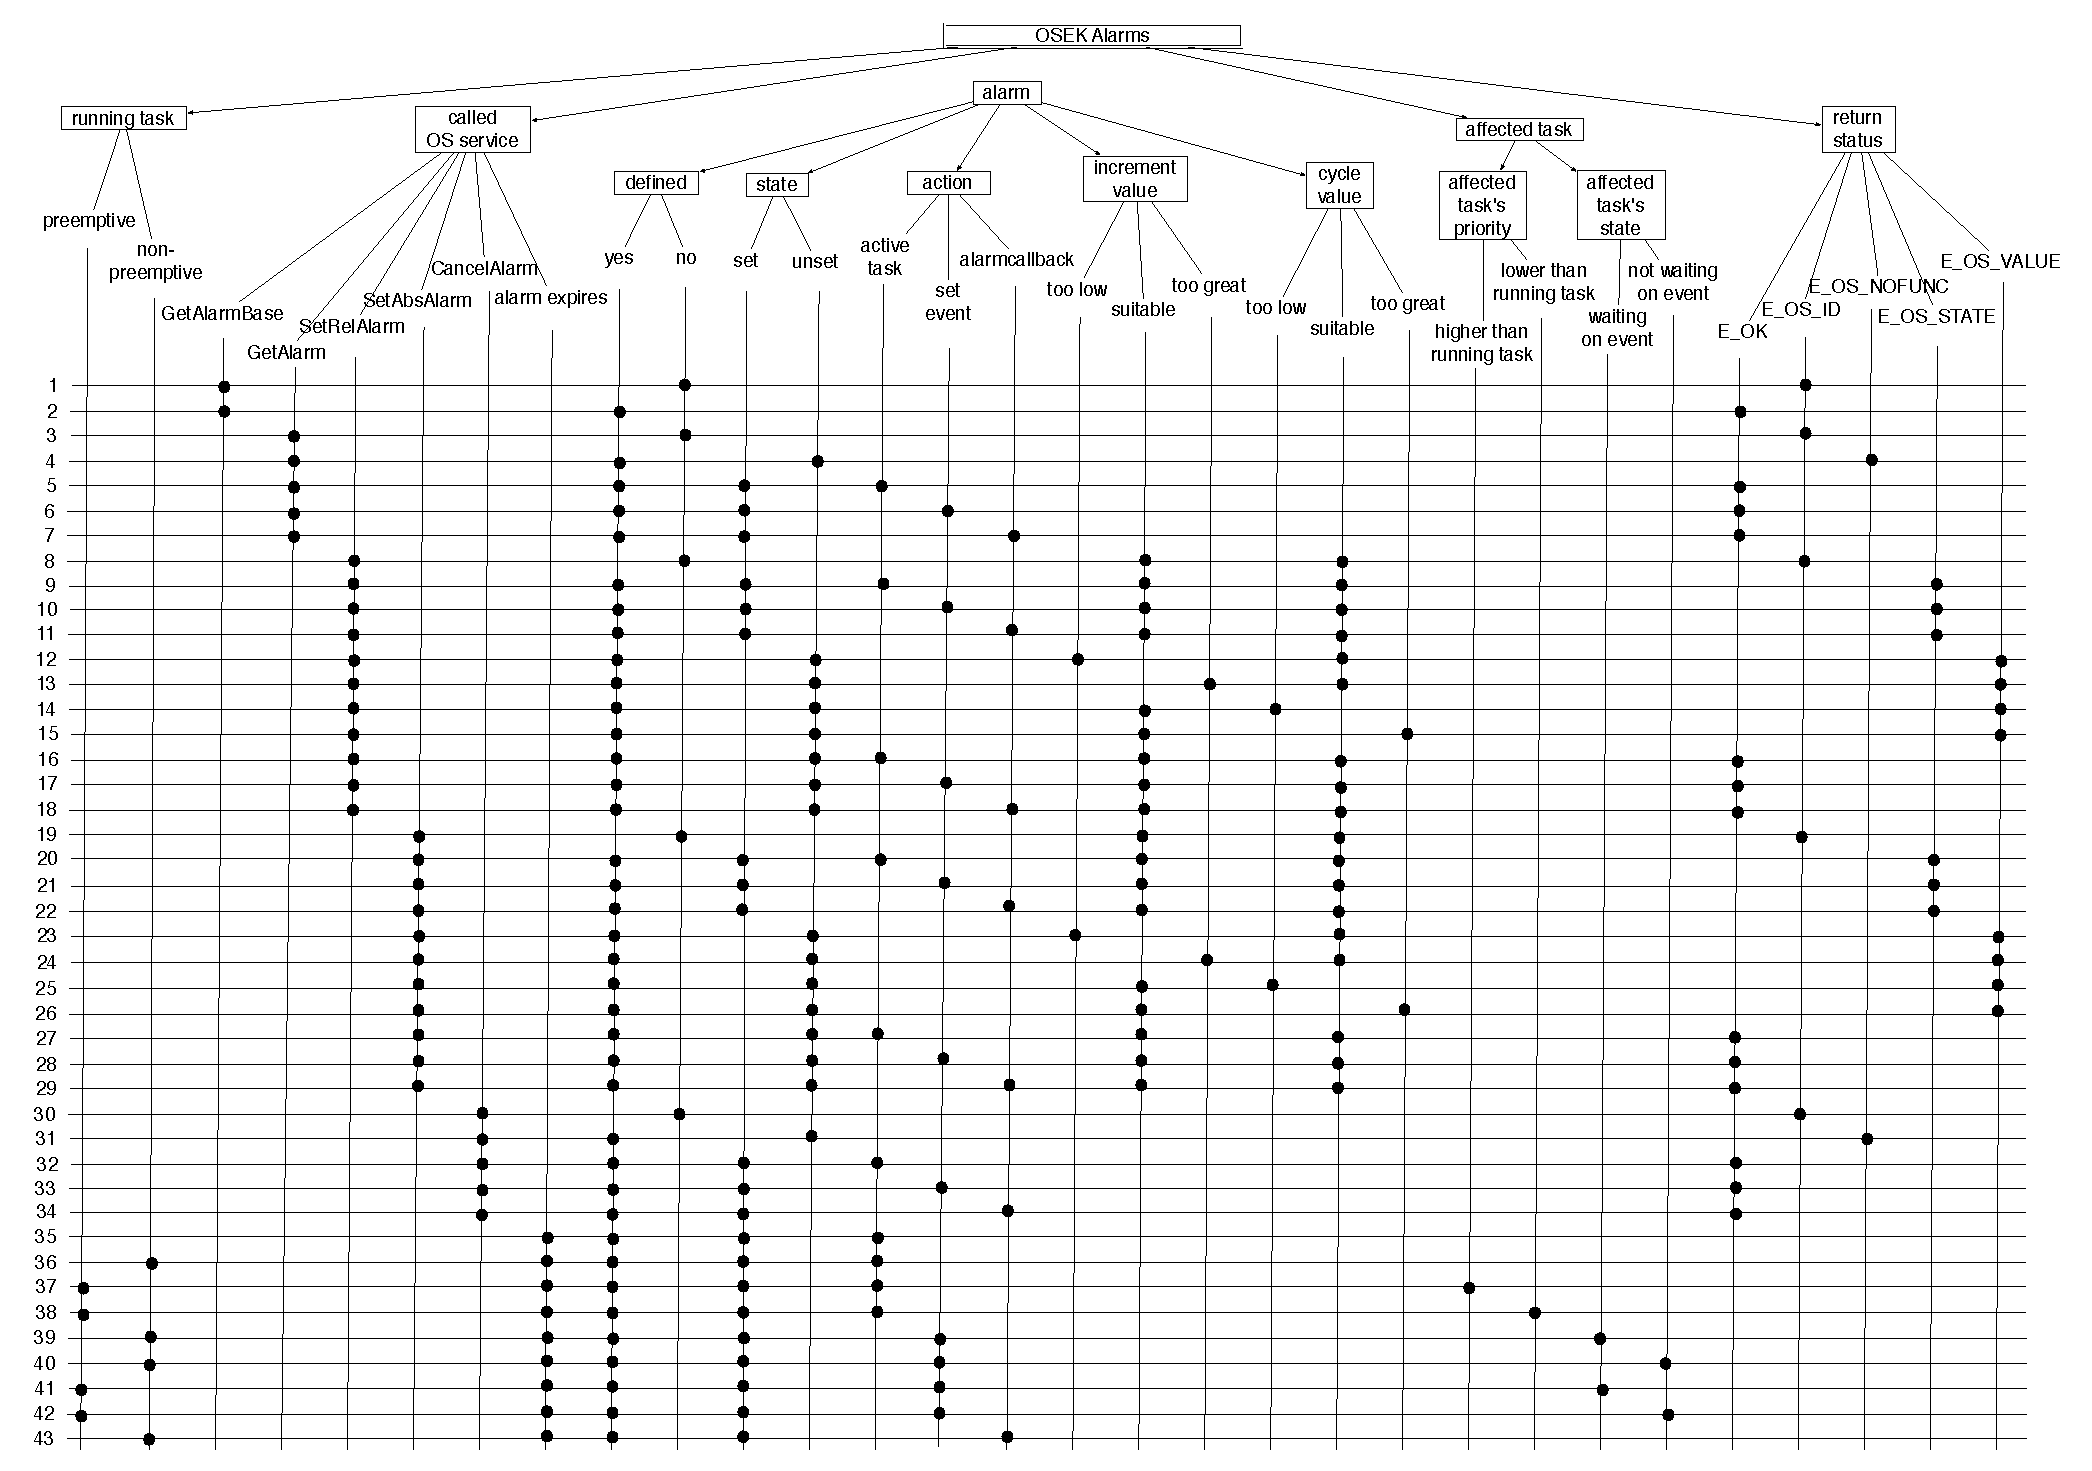
\includegraphics[width=1\textheight, angle=90]{graphics/OSEK_Alarms.pdf}
	\end{figure}
		
	\begin{supertabular}{|p{\Li}|p{\Lii}|p{\Liii}|} \hline
	1 	& Call GetAlarmBase() with invalid alarm ID 											& Service returns E\_OS\_ID \\ \hline
	2 	& Call GetAlarmBase() Return alarm base characteristics. 								& Service returns E\_OK \\ \hline
	3	& Call GetAlarm() with invalid alarm ID 												& Service returns E\_OS\_ID \\ \hline
	4	& Call GetAlarm() for alarm which is currently not in use									& Service returns E\_OS\_NOFUNC \\ \hline
	5	& Call GetAlarm() for alarm which will activate a task on expiration 							& Returns number of ticks until expiration. Service returns E\_OK \\ \hline
	6	& Call GetAlarm() for alarm which will set an event on expiration 							& Returns number of ticks until expiration. Service returns E\_OK \\ \hline
	7	& Call GetAlarm() for alarm which will callback a routine on expiration	 					& Returns number of ticks until expiration. Service returns E\_OK \\ \hline
	8	& Call SetRelAlarm() with invalid alarm ID 											& Service returns E\_OS\_ID \\ \hline
	9 	& Call SetRelAlarm() for already activated alarm which will activate a task on expiration			& Service returns E\_OS\_STATE \\ \hline
	10	& Call SetRelAlarm() for already activated alarm which will set an event on expiration 			& Service returns E\_OS\_STATE \\ \hline
	11	& Call SetRelAlarm() for already activated alarm which will callback a routine on expiration 		& Service returns E\_OS\_STATE \\ \hline
	12	& Call SetRelAlarm() with increment value lower than zero								& Service returns E\_OS\_VALUE \\ \hline
	13	& Call SetRelAlarm() with increment value greater than maxallowedvalue 					& Service returns E\_OS\_VALUE \\ \hline
	14 	& Call SetRelAlarm() with cycle value lower than mincycle 								& Service returns E\_OS\_VALUE \\ \hline
	15	& Call SetRelAlarm() with cycle value greater than maxallowedvalue 						& Service returns E\_OS\_VALUE \\ \hline
	16	& Call SetRelAlarm() for alarm which will activate a task on expiration 						& Alarm is activated. Service returns E\_OK \\ \hline
	17 	& Call SetRelAlarm() for alarm which will set an event on expiration 			 			& Alarm is activated.Service returns E\_OK \\ \hline
	18 	& Call SetRelAlarm() for alarm which will callback a routine on expiration 		 			& Alarm is activated.Service returns E\_OK \\ \hline
	19 	& Call SetAbsAlarm() with invalid alarm ID 											& Service returns E\_OS\_ID \\ \hline
	20	& Call SetAbsAlarm() for already activated alarm which will activate a task on expiration 			& Service returns E\_OS\_STATE \\ \hline
	21	& Call SetAbsAlarm() for already activated alarm which will set an event on expiration 			& Service returns E\_OS\_STATE \\ \hline
	22	& Call SetAbsAlarm() for already activated alarm which will callback a routine on expiration	 	& Service returns E\_OS\_STATE \\ \hline
	23	& Call SetAbsAlarm() with increment value lower than zero								& Service returns E\_OS\_VALUE \\ \hline
	24	& Call SetAbsAlarm() with increment value greater than maxallowedvalue 					& Service returns E\_OS\_VALUE \\ \hline
	25	& Call SetAbsAlarm() with cycle value lower than mincycle 								& Service returns E\_OS\_VALUE \\ \hline
	26 	& Call SetAbsAlarm() with cycle value greater than maxallowedvalue 						& Service returns E\_OS\_VALUE\\ \hline
	27	& Call SetAbsAlarm() for alarm	which will activate a task on expiration 						& Alarm is activated. Service returns E\_OK \\ \hline
	28	& Call SetAbsAlarm() for alarm which will set an event on expiration 						& Alarm is activated. Service returns E\_OK \\ \hline
	29	& Call SetAbsAlarm() for alarm which will callback a routine on expiration	 				& Alarm is activated. Service returns E\_OK \\ \hline
	30	& Call CancelAlarm() with invalid alarm ID 											& Service returns E\_OS\_ID \\ \hline
	31	& Call CancelAlarm() for alarm which is currently not in use								& Service returns E\_OS\_NOFUNC \\ \hline
	32 	& Call CancelAlarm() for already activated alarm which will activate a task on expiration 			& Alarm is cancelled. Service returns E\_OK\\ \hline 
	33 	& Call CancelAlarm() for already activated alarm which will set an event on expiration 			& Alarm is cancelled. Service returns E\_OK \\ \hline
	34 	& Call CancelAlarm() for already activated alarm which will callback a routine on expiration	 	& Alarm is cancelled. Service returns E\_OK \\ \hline
	35	& Expiration of alarm which activates a task while no tasks are currently running 				& Task is activated\\ \hline
	36 	& Expiration of alarm which activates a task while running task is non-preemptive 				& Task is activated. No preemption of running task \\ \hline
	37	& Expiration of alarm which activates a task with higher priority than running task while running task is preemptive 	& Task is activated. Task with highest priority is executed \\ \hline
	38	& Expiration of alarm which activates a task with lower priority than running task while running task is preemptive 	& Task is activated. No preemption of running task. \\ \hline
	39	& Expiration of alarm which sets an event while running task is non-preemptive. Task which owns the event is not waiting for this event and not suspended	& Event is set\\ \hline
	40	& Expiration of alarm which sets an event while running task is non-preemptive. Task which owns the event is waiting for this event	& Event is set. Task which is owner of the event becomes ready. No preemption of running task \\ \hline
	41 	& Expiration of alarm which sets an event while running task is preemptive. Task which owns the event is not waiting for this event and not suspended 	& Event is set\\ \hline
	42 	& Expiration of alarm which sets an event while running task is preemptive. Task which owns the event is waiting for this event	& Event is set. Task which is owner of the event becomes ready. Task with highest priority is executed (Rescheduling) \\ \hline
	43 	& Expiration of alarm which callback a routine 				 							& Running task becomes ready. Callback routine is activated. \\ \hline
	\end{supertabular} \\  
	
	% HOOK ROUTINES %
	\subsection{Error handling, hook routines (with interrupts) and OS execution control}
	The specification doesn’t provide an error status when calling an OS service which is not allowed on hook level from inside a hook routine. It is assumed that the correct behaviour would be to return E\_OS\_CALLEVEL. As this is not prescribed by the specification, this will not be used as a criteria for the conformance of the implementation. Anyway, the conformance tests will check that restricted OS services return a value not equal E\_OK.\\
	Compare to the previous Test Plan 2.0, it's forbidden to call ActivateTask() from StartupHook routine. SuspendAllInterrupts() and ResumeAllInterrupts() are allowed in hook routines.\\
	See Annexe \ref{interrupts_management} for more information about interrupt management (test case from 15 to 32).\\
	
	\begin{supertabular}{|p{\Li}|p{\Lii}|p{\Liii}|} \hline
	1	& Call GetActiveApplicationMode() 									& Return current application mode \\ \hline 
	2	& Call StartOS() 												& Start operating system \\ \hline 
	3	& Call ShutdownOS() 											& Shutdown operating system \\ \hline 
	4	& Check PreTaskHook/PostTaskHook: Force rescheduling				& PreTaskHook is called before executing the new task, but after the transition to running state. PostTaskHook is called after exiting the current task but before leaving the task’s running state \\ \hline 
	5	& Check ErrorHook: Force error 									& ErrorHook is called at the end of a system service which has a return value not equal E\_OK \\ \hline 
	6	& Check StartupHook: Start OS 									& StartupHook is called after initialisation of OS \\ \hline 
	7	& Check ShutdownHook: Shutdown OS 								& ShutdownHook is called after the OS shutdown \\ \hline 
		& \textit{Check availability of OS services inside hook routines according to fig 12-1 of OS spec.} & \textit{OS services which must not be called from hook routines return status not equal E\_OK} \\ \hline
	8	& Call GetTaskID() from ErrorHook, PreTaskHook and PostTaskHook		& Return E\_OK \\ \hline 
	9	& Call GetTaskState() from ErrorHook, PreTaskHook and PostTaskHook		& Return E\_OK if TaskID is valid \\ \hline 
	10	& Call SuspendAllInterrupts() from ErrorHook, PreTaskHook and PostTaskHook	& \\ \hline 
	11	& Call ResumeAllInterrupts() from ErrorHook, PreTaskHook and PostTaskHook	& \\ \hline 
	12	& Call GetEvent() from ErrorHook, PreTaskHook and PostTaskHook		& Return E\_OK if TaskID is valid, Referenced task $<$TaskID$>$ is an extended task and not in suspended state. \\ \hline
	13	& Call GetAlarmBase() from ErrorHook, PreTaskHook and PostTaskHook	& Return E\_OK if AlarmID is valid \\ \hline 
	14	& Call GetAlarm() from ErrorHook, PreTaskHook and PostTaskHook		& Return E\_OK if AlarmID is valid and used \\ \hline
	\multicolumn{3}{|l|}{ 	\textbf{Interrupt processing in Hook routines :} }\\ \hline
	15 	& \multicolumn{2}{|p{\Liiii}|}{ Interrupt activation in PostTaskHook of a task preempted by an alarm which activate a task.} \\ \hline
	16 	& \multicolumn{2}{|p{\Liiii}|}{Interrupt activation in PreTaskHook of a task preempted by an alarm which activate a task.} \\ \hline
	17 	& \multicolumn{2}{|p{\Liiii}|}{Interrupt activation in PostTaskHook of a task preempted by an ISR2.} \\ \hline
	18 	& \multicolumn{2}{|p{\Liiii}|}{Interrupt activation in PreTaskHook of a task preempted by an ISR2.} \\ \hline
	19 	& \multicolumn{2}{|p{\Liiii}|}{Interrupt activation in PostTaskHook of a task activated by an task (preempted or not).} \\ \hline
	20 	& \multicolumn{2}{|p{\Liiii}|}{Interrupt activation in PreTaskHook of a task activated by an task (preempted or not).} \\ \hline
	21 	& \multicolumn{2}{|p{\Liiii}|}{Interrupt activation in PostTaskHook of a task activated by an alarm which will give back the hand to the previous running task.} \\ \hline
	22 	& \multicolumn{2}{|p{\Liiii}|}{Interrupt activation in PreTaskHook of a task activated by an alarm which will give back the hand to the previous running task.} \\ \hline
	23 	& \multicolumn{2}{|p{\Liiii}|}{Interrupt activation in PostTaskHook of an ISR2 which will give back the hand to the previous running task.} \\ \hline
	24 	& \multicolumn{2}{|p{\Liiii}|}{Interrupt activation in PreTaskHook of an ISR2 which will give back the hand to the previous running task.} \\ \hline
	
	25 	& \multicolumn{2}{|p{\Liiii}|}{ Interrupt triggering with an activation in PostTaskHook of a task preempted by an alarm which activate a task.} \\ \hline
	26 	& \multicolumn{2}{|p{\Liiii}|}{Interrupt triggering with an activation in PreTaskHook of a task preempted by an alarm which activate a task.} \\ \hline
	27 	& \multicolumn{2}{|p{\Liiii}|}{Interrupt triggering with an activation in PostTaskHook of a task preempted by an ISR2.} \\ \hline
	28 	& \multicolumn{2}{|p{\Liiii}|}{Interrupt triggering with an activation in PreTaskHook of a task preempted by an ISR2.} \\ \hline
	29 	& \multicolumn{2}{|p{\Liiii}|}{Interrupt triggering with an activation in PostTaskHook of a task followed by an task (preempted or not).} \\ \hline
	30 	& \multicolumn{2}{|p{\Liiii}|}{Interrupt triggering with an activation in PreTaskHook of a task followed by an task (preempted or not).} \\ \hline
	31 	& \multicolumn{2}{|p{\Liiii}|}{Interrupt triggering with an activation in PostTaskHook of a task activated by an alarm which will give back the hand to the previous running task.} \\ \hline
	32 	& \multicolumn{2}{|p{\Liiii}|}{Interrupt triggering with an activation in PreTaskHook of a task activated by an alarm which will give back the hand to the previous running task.} \\ \hline
	33 	& \multicolumn{2}{|p{\Liiii}|}{Interrupt triggering with an activation in PostTaskHook of an ISR2 which will give back the hand to the previous running task.} \\ \hline
	34 	& \multicolumn{2}{|p{\Liiii}|}{Interrupt triggering with an activation in PreTaskHook of an ISR2 which will give back the hand to the previous running task.} \\ \hline
	35	& \multicolumn{2}{|p{\Liiii}|}{Interrupt activation in ErrorHook.} \\ \hline
	36	& \multicolumn{2}{|p{\Liiii}|}{Interrupt triggering with an activation in ErrorHook.} \\ \hline
	\end{supertabular} \\  
	
	% Internal COM %
	\subsection{Internal COM}
	
	\begin{figure}[htbp] %  figure placement: here, top, bottom, or page
   		\centering
		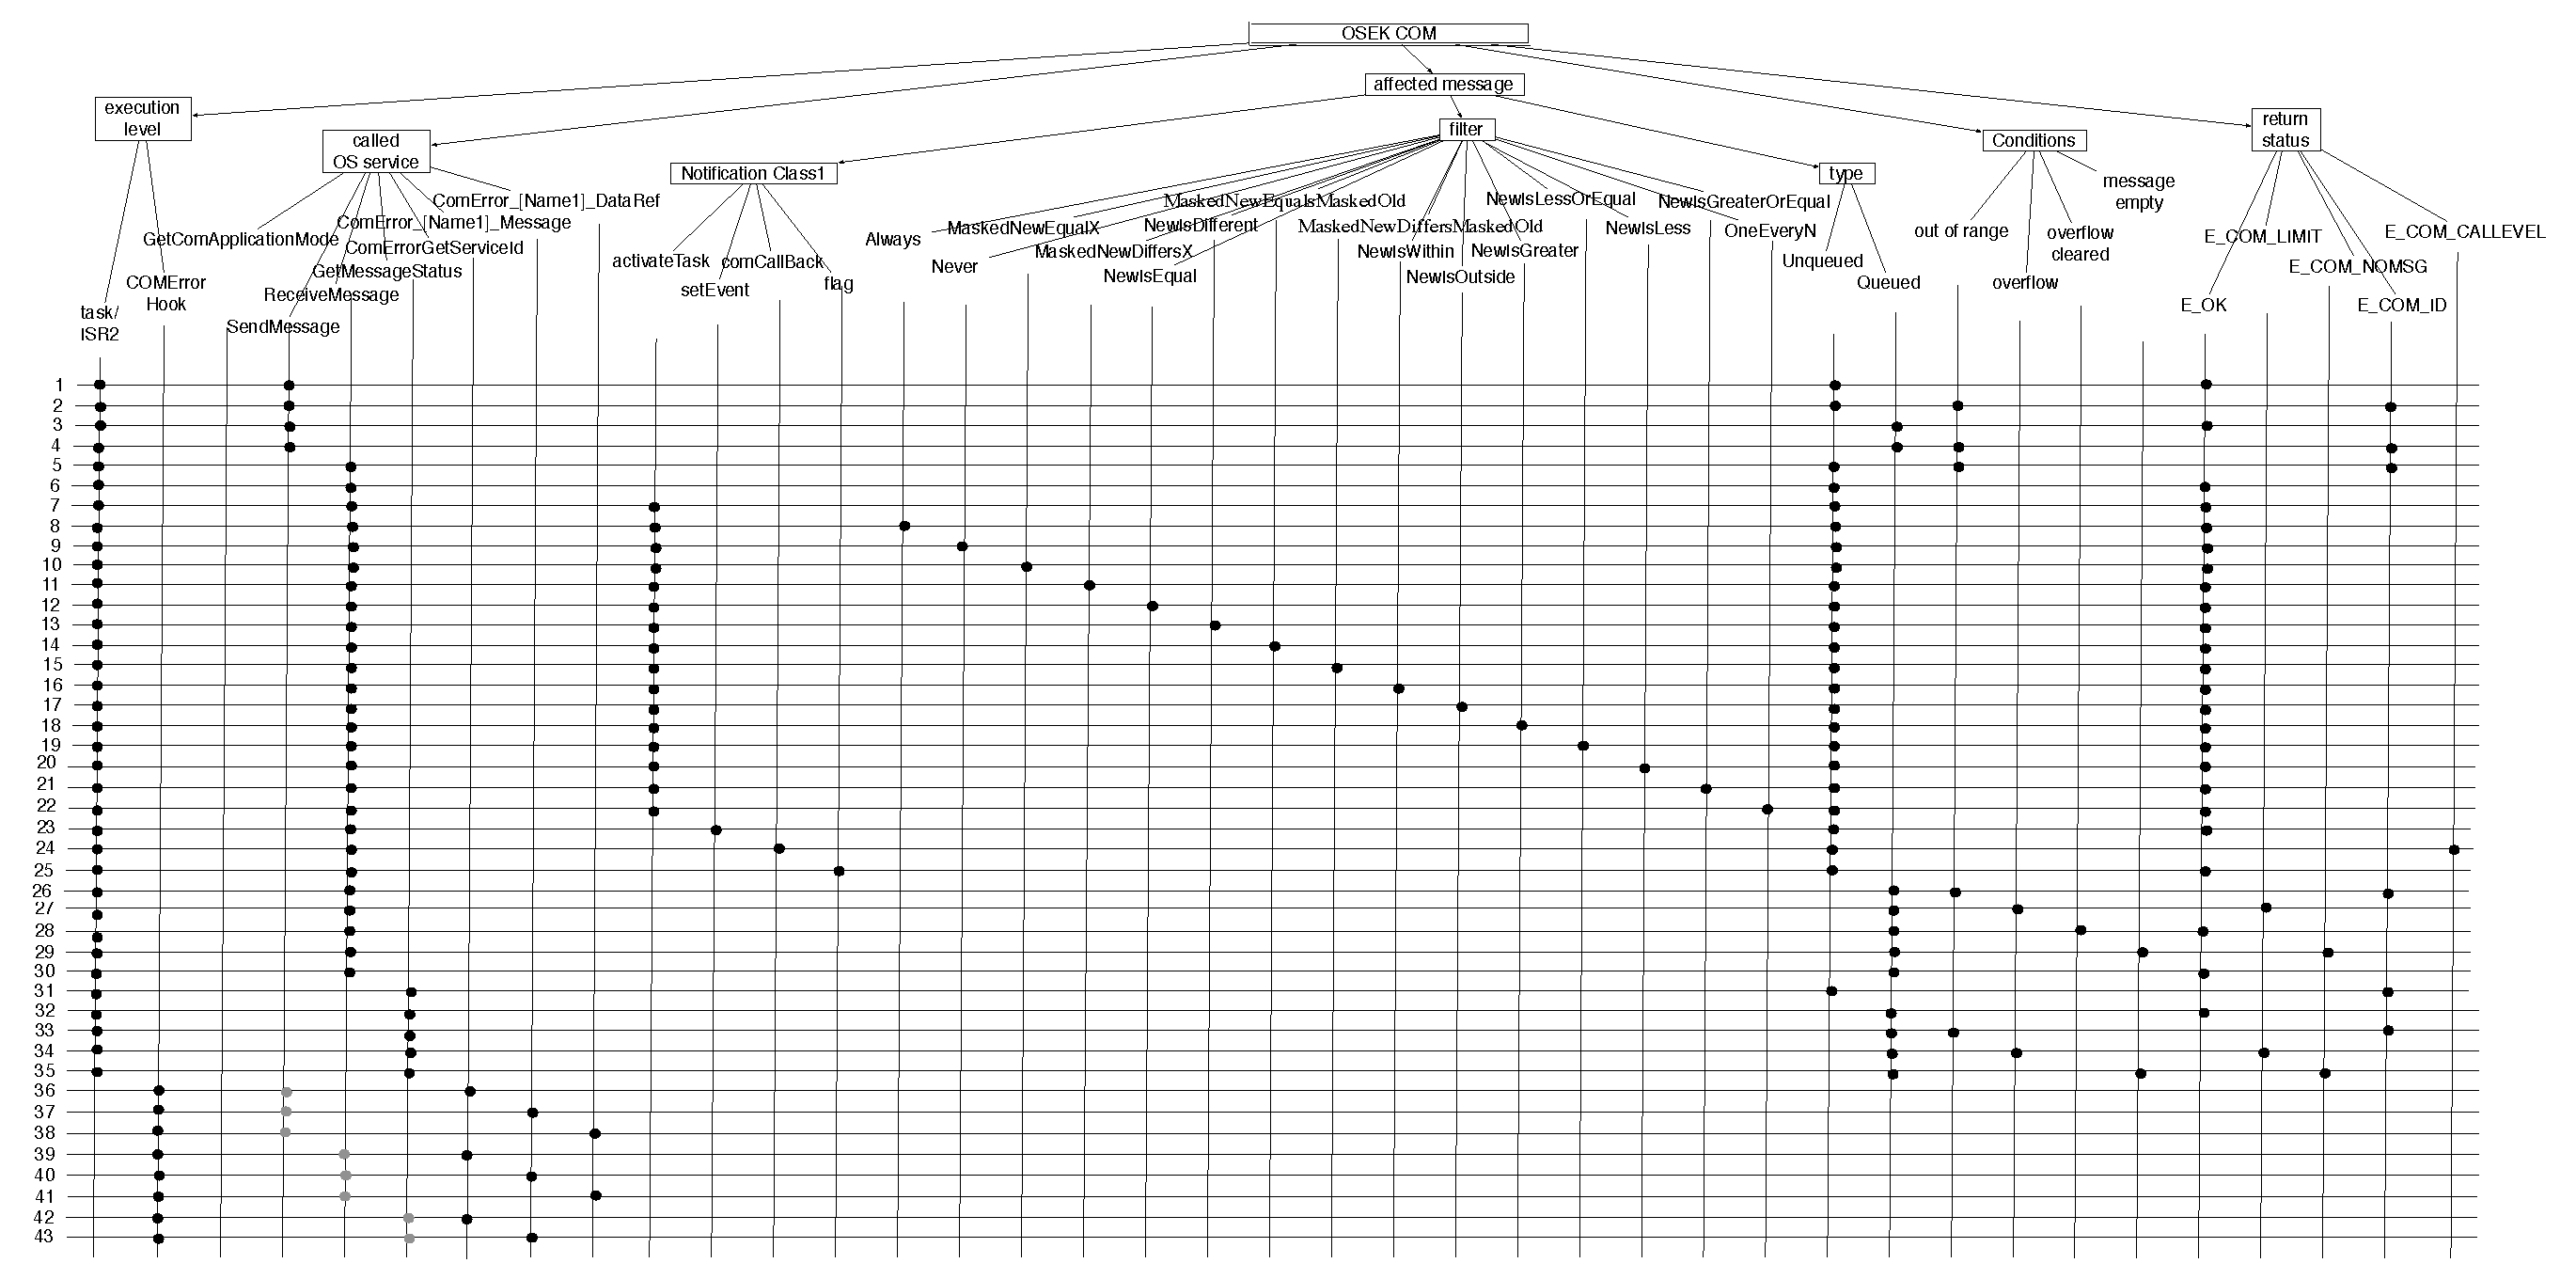
\includegraphics[width=1\textheight, angle=90]{graphics/OSEK_Internal_COM.pdf}
	\end{figure}

\setlength{\Lii}{10cm}
\setlength{\Liii}{\textwidth} \addtolength{\Liii}{-\Li} \addtolength{\Liii}{-\Lii}

	\begin{supertabular}{|p{\Li}|p{\Lii}|p{\Liii}|} \hline
	1	& Call SendMessage() to an unqueued message										& Service returns E\_OK \\ \hline
	2	& Call SendMessage() to an unqueued message with $<$Message$>$ out of range				& Service returns E\_COM\_ID \\ \hline
	3	& Call SendMessage() to a queued message											& Service returns E\_OK \\ \hline
	4	& Call SendMessage() to a queued message with $<$Message$>$ out of range					& Service returns E\_COM\_ID \\ \hline
	5	& Call ReceiveMessage() to an unqueued message with $<$Message$>$ out of range				& Service returns E\_COM\_ID \\ \hline
	6	& Call ReceiveMessage() to an unqueued message									& Service returns E\_OK \\ \hline
	7	& Call ReceiveMessage() to an unqueued message with a notification which activate a task		& Service returns E\_OK \\ \hline
	8	& Call ReceiveMessage() to an unqueued message with a notification which activate a task and a "always" filter		& Service returns E\_OK \\ \hline
	9	& Call ReceiveMessage() to an unqueued message with a notification which activate a task and a "never" filter		& Service returns E\_OK \\ \hline
	10	& Call ReceiveMessage() to an unqueued message with a notification which activate a task and a "MaskedNewEqualX" filter		& Service returns E\_OK \\ \hline
	11	& Call ReceiveMessage() to an unqueued message with a notification which activate a task and a "MaskedNewDiffersX" filter		& Service returns E\_OK \\ \hline
	12	& Call ReceiveMessage() to an unqueued message with a notification which activate a task and a "NewIsEqual" filter		& Service returns E\_OK \\ \hline
	13	& Call ReceiveMessage() to an unqueued message with a notification which activate a task and a "NewIsDifferent" filter		& Service returns E\_OK \\ \hline
	14	& Call ReceiveMessage() to an unqueued message with a notification which activate a task and a "MaskedNewEqualsMaskedOld" filter		& Service returns E\_OK \\ \hline
	15	& Call ReceiveMessage() to an unqueued message with a notification which activate a task and a "MaskedNewEqualsMaskedOld" filter		& Service returns E\_OK \\ \hline
	16	& Call ReceiveMessage() to an unqueued message with a notification which activate a task and a "NewIsWithin" filter		& Service returns E\_OK \\ \hline
	17	& Call ReceiveMessage() to an unqueued message with a notification which activate a task and a "NewIsOutside" filter		& Service returns E\_OK \\ \hline
	18	& Call ReceiveMessage() to an unqueued message with a notification which activate a task and a "NewIsGreater" filter		& Service returns E\_OK \\ \hline
	19	& Call ReceiveMessage() to an unqueued message with a notification which activate a task and a "NewIsLessOrEqual" filter		& Service returns E\_OK \\ \hline
	20	& Call ReceiveMessage() to an unqueued message with a notification which activate a task and a "NewIsLess" filter		& Service returns E\_OK \\ \hline
	21	& Call ReceiveMessage() to an unqueued message with a notification which activate a task and a "NewIsGreaterOrEqual" filter		& Service returns E\_OK \\ \hline
	22	& Call ReceiveMessage() to an unqueued message with a notification which activate a task and a "OneEveryN" filter		& Service returns E\_OK \\ \hline
	23	& Call ReceiveMessage() to an unqueued message with a notification which set an event		& Service returns E\_OK \\ \hline
	24	& Call ReceiveMessage() to an unqueued message with a notification which callback a routine	& Service returns E\_COM\_CALLEVEL \\ \hline
	25	& Call ReceiveMessage() to an unqueued message with a notification which set a flag			& Service returns E\_OK \\ \hline
	26	& Call ReceiveMessage() to a queued message with $<$Message$>$ out of range					& Service returns E\_COM\_ID \\ \hline
	27	& Call ReceiveMessage() to a queued message which had an overflow on last SendMessage	& Service returns E\_COM\_LIMIT and reset the overflow flag \\ \hline
	28	& Call ReceiveMessage() to a queued message which had an overflow cleared on last call to ReceiveMessage	& Service returns E\_OK \\ \hline
	29	& Call ReceiveMessage() to a queued message which is empty							& Service returns E\_COM\_NOMSG \\ \hline
	30	& Call ReceiveMessage() to a queued message										& Service returns E\_OK \\ \hline
	31	& Call GetMessageStatus() to an unqueued message									& Service returns E\_COM\_ID \\ \hline
	32	& Call GetMessageStatus() to a queued message										& Service returns E\_OK \\ \hline
	33	& Call GetMessageStatus() to a queued message with $<$Message$>$ out of range				& Service returns E\_COM\_ID \\ \hline
	34	& Call GetMessageStatus() to a queued message which had an overflow on last SendMessage	& Service returns E\_COM\_LIMIT \\ \hline
	35	& Call GetMessageStatus() to a queued message which is empty							& Service returns E\_COM\_NOMSG \\ \hline
	36	& Call ComErrorGetServiceId() from ComErrorHook with SendMessage error					& Service returns COMServiceId\_SendMessage \\ \hline
	37	& Call ComError\_SendMessage\_Message from ComErrorHook 							& Service returns $<$Message$>$ used in last SendMessage \\ \hline
	38	& Call ComError\_SendMessage\_DataRef from ComErrorHook 							& Service returns $<$DataRef$>$ used in last SendMessage \\ \hline
	39	& Call ComErrorGetServiceId() from ComErrorHook with ReceiveMessage error				& Service returns COMServiceId\_ReceiveMessage \\ \hline
	40	& Call ComError\_ReceiveMessage\_Message from ComErrorHook 							& Service returns $<$Message$>$ used in last ReceiveMessage \\ \hline
	41	& Call ComError\_ReceiveMessage\_DataRef from ComErrorHook 							& Service returns $<$DataRef$>$ used in last ReceiveMessage \\ \hline
	42	& Call ComErrorGetServiceId() from ComErrorHook with GetMessageStatus error				& Service returns COMServiceId\_GetMessageStatus \\ \hline
	43	& Call ComError\_GetMessageStatus\_Message from ComErrorHook 						& Service returns $<$Message$>$ used in last GetMessageStatus \\ \hline
	\end{supertabular} \\  


	% AUTOSAR - CORE OS %
	\subsection{AUTOSAR - Core OS}
	OS Requirements : 263*, 264*, 285, 301, 304, 321\\
	Test cases 3 and  5 are GOIL test cases. Test case 7 is impossible to test.\\
	
	\begin{figure}[htbp] %  figure placement: here, top, bottom, or page
   		\centering
		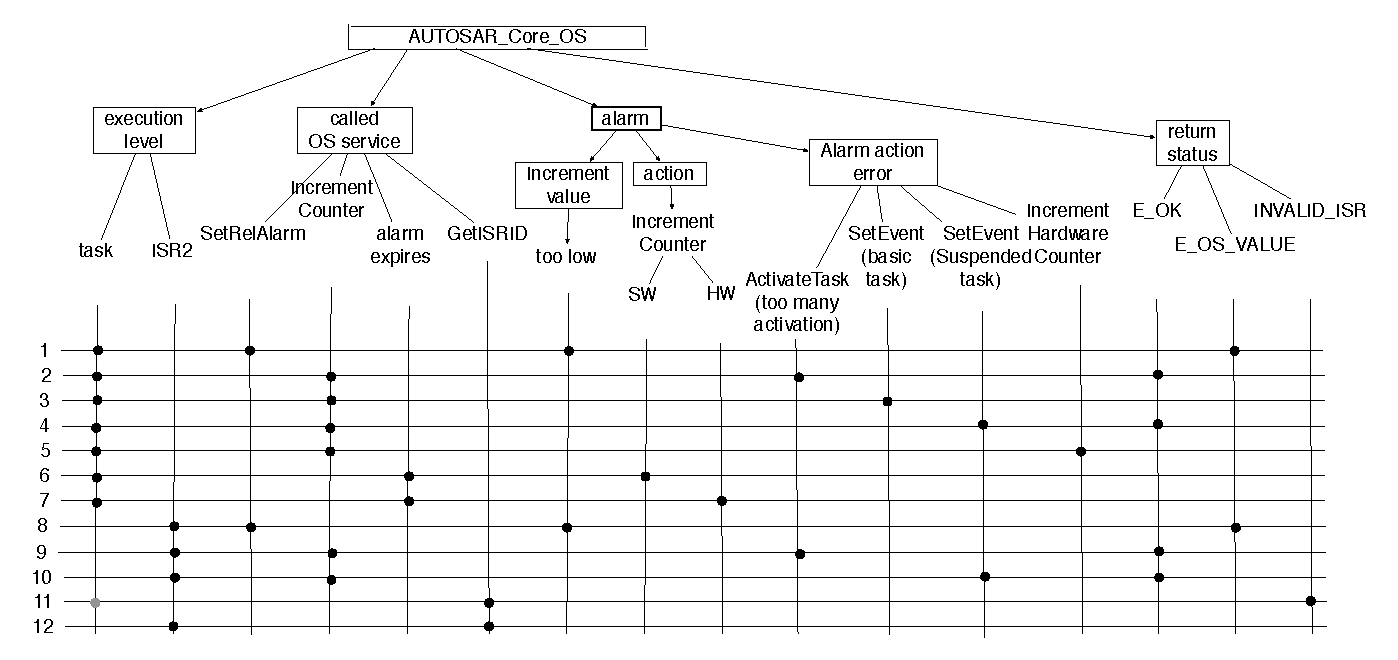
\includegraphics[width=1\textwidth, angle=0]{graphics/AUTOSAR_Core_OS.pdf}
	\end{figure}


\newlength{\Liiiii}\setlength{\Liiiii}{2,5cm}
\setlength{\Lii}{10cm}
\setlength{\Liii}{\textwidth} \addtolength{\Liii}{-\Li} \addtolength{\Liii}{-\Lii} \addtolength{\Liii}{-\Liiiii}
\tablefirsthead{ \hline \rowcolor{lightgray} Test Case No. & Action & Expected Result  & OS Requirements\\ }
\tablehead{ \hline \rowcolor{lightgray} Test Case No. & Action & Expected Result & OS Requirements \\}


	\begin{supertabular}{|p{\Li}|p{\Lii}|p{\Liii}|p{\Liiiii}|} \hline
	1	& Call SetRelAlarm() from task with $<$increment$>$ value equal to zero 					&Service returns E\_OS\_VALUE						& OS304\\ \hline 
	2	& Call IncrementCounter() of a software counter from task (alarm action results in an error : ActivateTask() on a task which has already its max number of activation)	
																					&Errorhook is called. Service returns E\_OK				& OS321 \\ \hline
	3	& It is impossible to call IncrementCounter() setting an event from an alarm expiration to a basic task. & error : An alarm can't set an Event to a basic task (Task t1 is a basic task). 	& OS321 \\ \hline
	4	& Call IncrementCounter() of a software counter from task (alarm action results in an error : SetEvent() on a task is suspended)	
																					&Errorhook is called. Service returns E\_OK				& OS321 \\ \hline
	5	& It is impossible to call IncrementCounter() incrementing a hardware counter from an alarm expiration. 	& error : It is impossible to increment a hardware counter (Z is not a software counter). 			& OS285 \\ \hline
	6	& Expiration of alarm which increment a software counter					 				& Software counter is incremented and alarm(s) is(are) launched if needed & OS301 \\ \hline
	7	& Increment a hardware counter from an alarm expiration is impossible. GOIL generation should forbid to create an alarm which increment a hardware counter
																	 				& 												& \\ \hline
	8	& Call SetRelAlarm() from ISR2 with $<$increment$>$ value equal to zero 						&Service returns E\_OS\_VALUE						& OS304\\ \hline 
	9	& Call IncrementCounter() of a software counter from ISR2 (alarm action results in an error : ActivateTask() on a task which has already its max number of activation)	
																					&Errorhook is called. Service returns E\_OK				& OS321 \\ \hline
	10	& Call IncrementCounter() of a software counter from ISR2 (alarm action results in an error : SetEvent() on a task is suspended)	
																					&Errorhook is called. Service returns E\_OK				& OS321 \\ \hline
	11	& Call GetISRID() from an other object than ISR2 or Hook routine called inside an ISR2 			& Service returns INVALID\_ISR						& OS264 \\ \hline
	12	& Call GetISRID() from an ISR2										 			& Service returns the identifier of the currently running ISR2	& OS263 \\ \hline
	\end{supertabular} \\  
	
	% AUTOSAR - SOFTWARE COUNTER %
	\subsection{AUTOSAR - Software Counter}
	OS Requirements : 285, 286, 321,376, 377, 381, 382, 383, 391, 392, 399, 460\\
	OS374 and  OS384 are indirectly tested thanks to the good fonctionning of the counter.\\ 
	
	\begin{figure}[htbp] %  figure placement: here, top, bottom, or page
   		\centering
		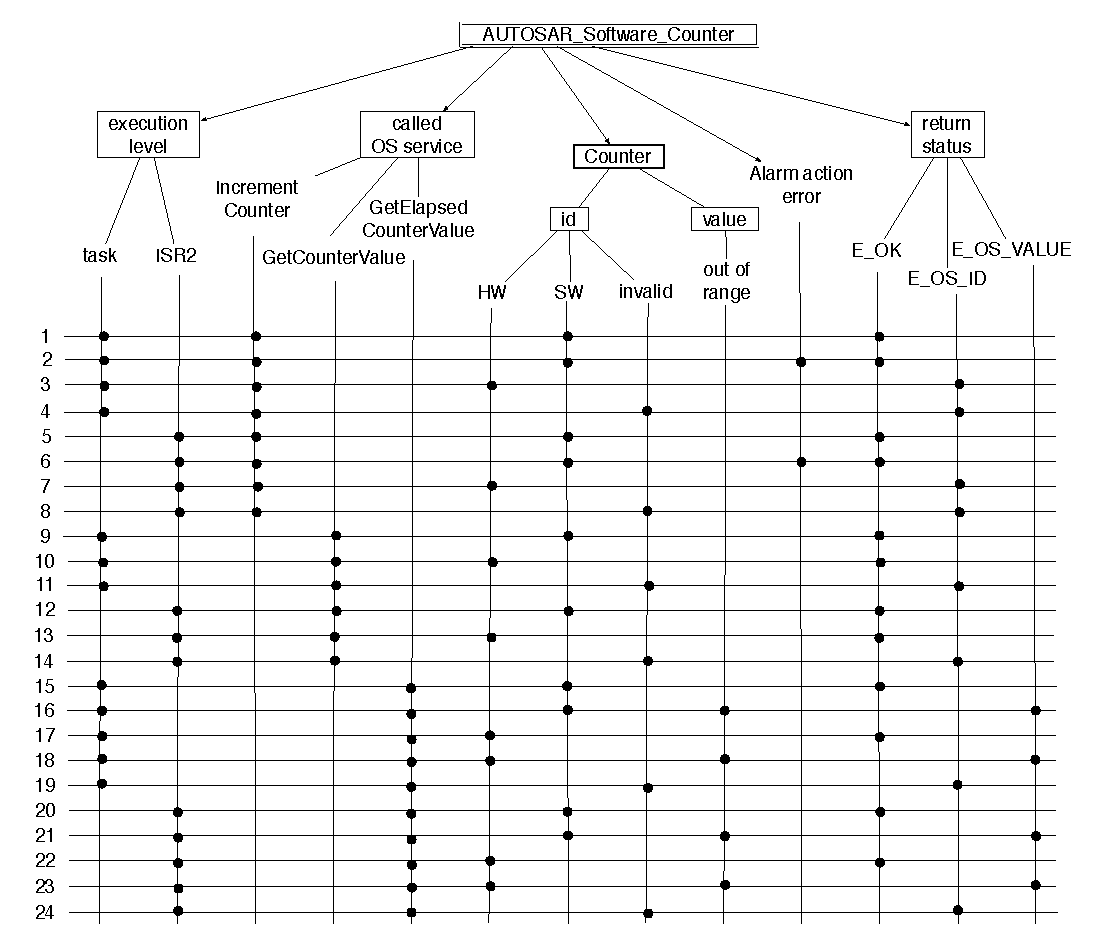
\includegraphics[width=1\textwidth, angle=0]{graphics/AUTOSAR_Software_Counter.pdf}
	\end{figure}

\setlength{\Lii}{7cm}
\setlength{\Liii}{\textwidth} \addtolength{\Liii}{-\Li} \addtolength{\Liii}{-\Lii} \addtolength{\Liii}{-\Liiiii}


	\begin{supertabular}{|p{\Li}|p{\Lii}|p{\Liii}|p{\Liiiii}|} \hline
	1	& Call IncrementCounter() of a software counter from task 								&Service returns E\_OK 								& OS286, OS399\\ \hline 
	2	& Call IncrementCounter() of a software counter from task (alarm action results in an error)		&Errorhook is called. Service returns E\_OK				& OS321 \\ \hline 
	3	& Call IncrementCounter() of a hardware counter from task 								&Service returns E\_OS\_ID							& OS285 \\ \hline 
	4	& Call IncrementCounter() from task with invalid ID										&Service returns E\_OS\_ID							& OS285 \\ \hline 
	5	& Call IncrementCounter() of a software counter from ISR2 								&Service returns E\_OK 								& \\ \hline 
	6	& Call IncrementCounter() of a software counter from ISR2 (alarm action results in an error)		&Errorhook is called. Service returns E\_OK 				& \\ \hline 
	7	& Call IncrementCounter() of a hardware counter from ISR2 								&Service returns E\_OS\_ID 							& \\ \hline 
	8	& Call IncrementCounter() from ISR2 with invalid ID										&Service returns E\_OS\_ID 							& \\ \hline 
	9	& Call GetCounterValue() of a sofwtare counter from task									& Service returns E\_OK and $<$Value$>$ of the counter	& OS377, OS383 \\ \hline 
	10	& Call GetCounterValue() of a hardware counter from task								& Service returns E\_OK and $<$Value$>$ of the counter	& OS377, OS383 \\ \hline 
	11	& Call GetCounterValue() from task with invalid ID										& Service returns E\_OS\_ID 							& OS376\\ \hline 
	12	& Call GetCounterValue() of a sofwtare counter from ISR2								& Service returns E\_OK and $<$Value$>$ of the counter	& \\ \hline 
	13	& Call GetCounterValue() of a hardware counter from ISR2								& Service returns E\_OK and $<$Value$>$ of the counter	& \\ \hline 
	14	& Call GetCounterValue() from ISR2 with invalid ID										& Service returns E\_OS\_ID 							& \\ \hline 
	15	& Call GetElapsedCounterValue() of a software counter from task							& Service returns E\_OK, the $<$Value$>$ of the counter and the number of elapsed ticks since the given $<$Value$>$ value via $<$ElapsedValue$>$																							& OS382, OS392, OS460 \\ \hline 
	16	& Call GetElapsedCounterValue() of a software counter from task with $<$Value$>$ out of range	& Service returns E\_OS\_VALUE						& OS391\\ \hline 
	17	& Call GetElapsedCounterValue() of a hardware counter from task							& Service returns E\_OK, the $<$Value$>$ of the counter and the number of elapsed ticks since the given $<$Value$>$ value via $<$ElapsedValue$>$																							& OS382, OS392, OS460\\ \hline 
	18	& Call GetElapsedCounterValue() of a hardware counter from task with $<$Value$>$ out of range	& Service returns E\_OS\_VALUE 						& OS391 \\ \hline 
	19	& Call GetElapsedCounterValue() from task with invalid ID								& Service returns E\_OS\_ID 							& OS381\\ \hline 
	20	& Call GetElapsedCounterValue() of a software counter from ISR2							& Service returns E\_OK, the $<$Value$>$ of the counter and the number of elapsed ticks since the given $<$Value$>$ value via $<$ElapsedValue$>$ 																							& \\ \hline 
	21	& Call GetElapsedCounterValue() of a software counter from ISR2 with $<$Value$>$ out of range	& Service returns E\_OS\_VALUE 						& \\ \hline 
	22	& Call GetElapsedCounterValue() of a hardware counter from ISR2							& Service returns E\_OK, the $<$Value$>$ of the counter and the number of elapsed ticks since the given $<$Value$>$ value via $<$ElapsedValue$>$ 																							& \\ \hline 
	23	& Call GetElapsedCounterValue() of a hardware counter from ISR2 with $<$Value$>$ out of range	& Service returns E\_OS\_VALUE 					& \\ \hline 
	24	& Call GetElapsedCounterValue() from ISR2 with invalid ID								& Service returns E\_OS\_ID 							& \\ \hline 
	\end{supertabular} \\  

	% AUTOSAR - SCHEDULE TABLE %
	\subsection{AUTOSAR - Schedule Table}
	OS Requirements : 002, 006, 007, 009, 191, 194, 275, (276), 277, 278, 279, 280, 281, 282, 283, 284, 289, 291, 293, 309, 324, 330, 332, 347, 348, 349, 350, 351, 353, 358, 359, 410, 412, 414, 428, 453.\\
	OS Requirements 401, 402, 403, 404, 407, 408, 409, 427, 442, 443, 444 are GOIL test cases (Test cases 33 to 42 and 70).\\
	OS411 can't be tested. As a schedule table is automatically set to single-shot if not specified, OS413 can't be tested.\\
	
	\begin{figure}[htbp] %  figure placement: here, top, bottom, or page
   		\centering
		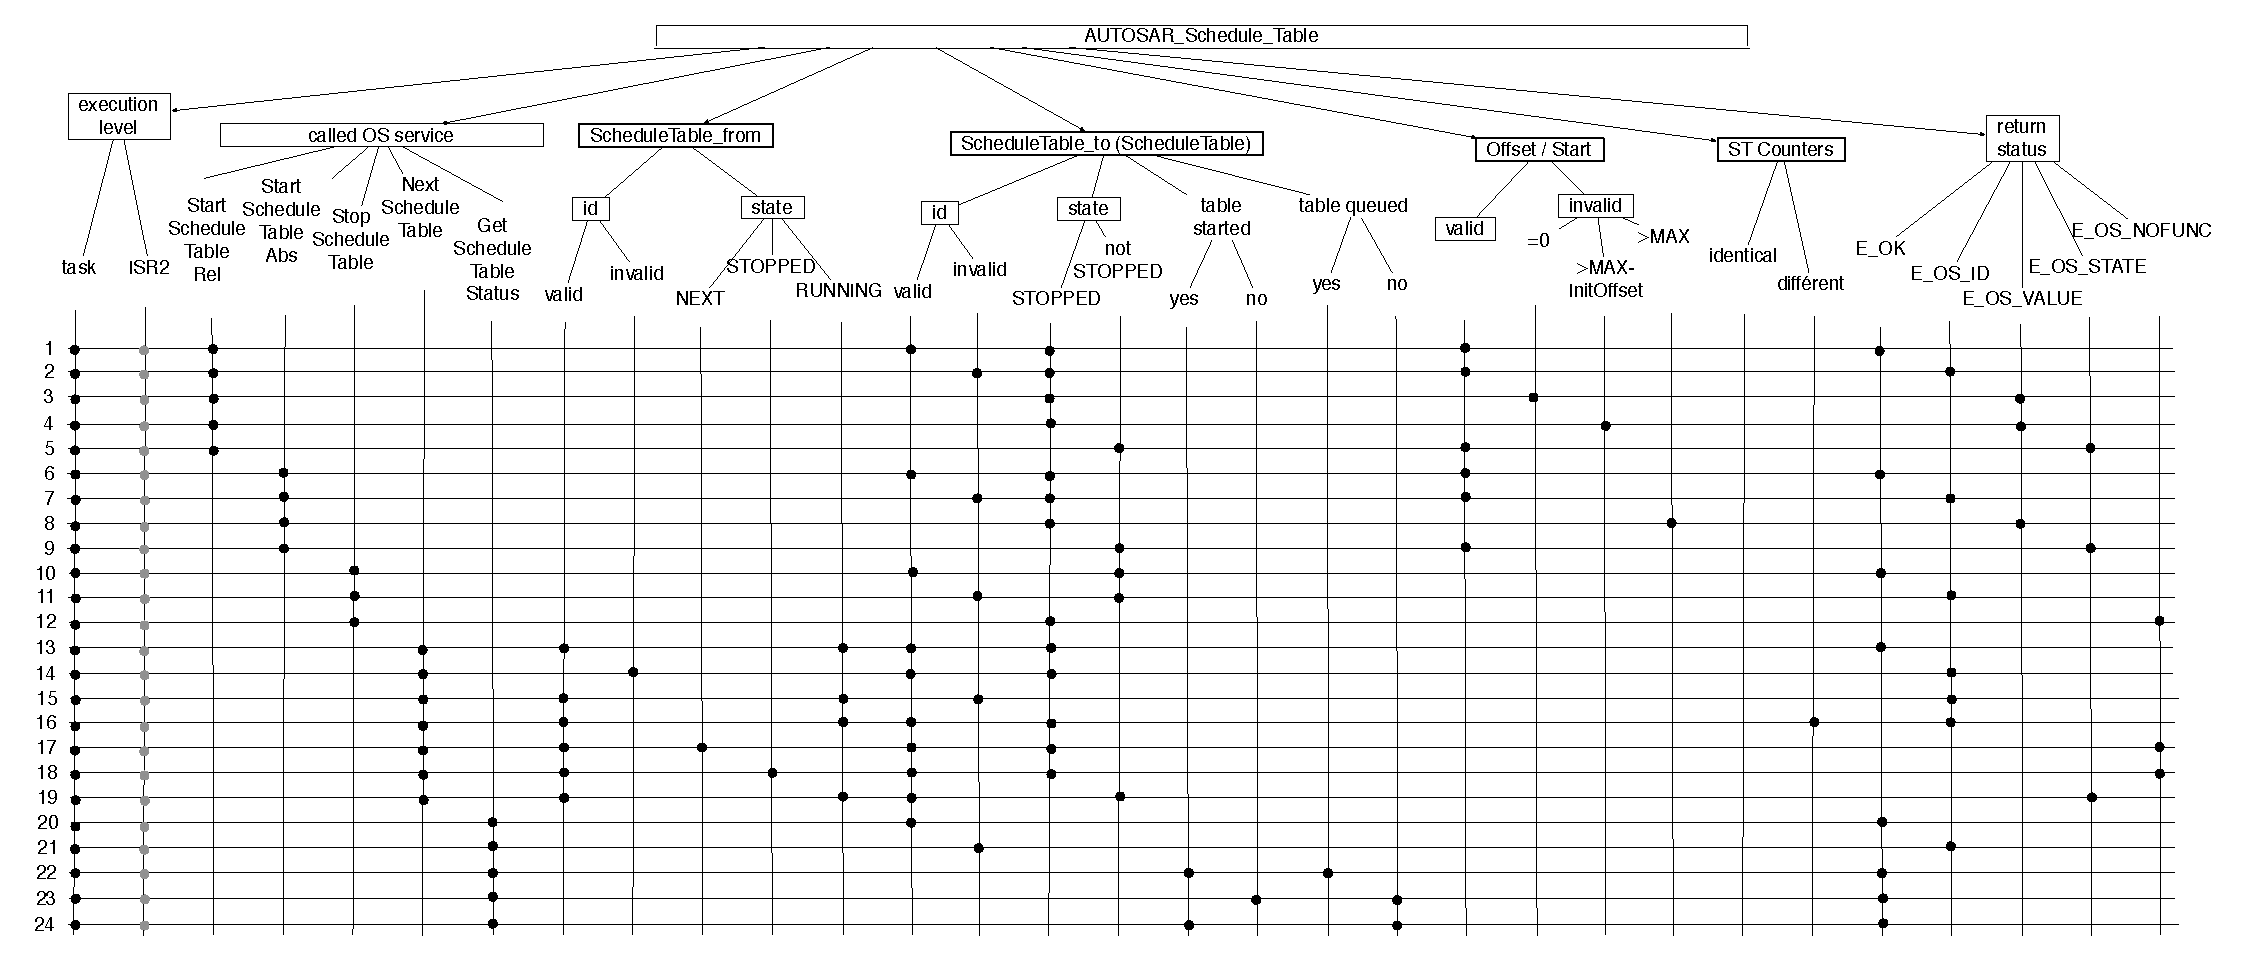
\includegraphics[width=1\textheight, angle=90]{graphics/AUTOSAR_Schedule_Table.pdf}
	\end{figure}

	\begin{figure}[htbp] %  figure placement: here, top, bottom, or page
   		\centering
		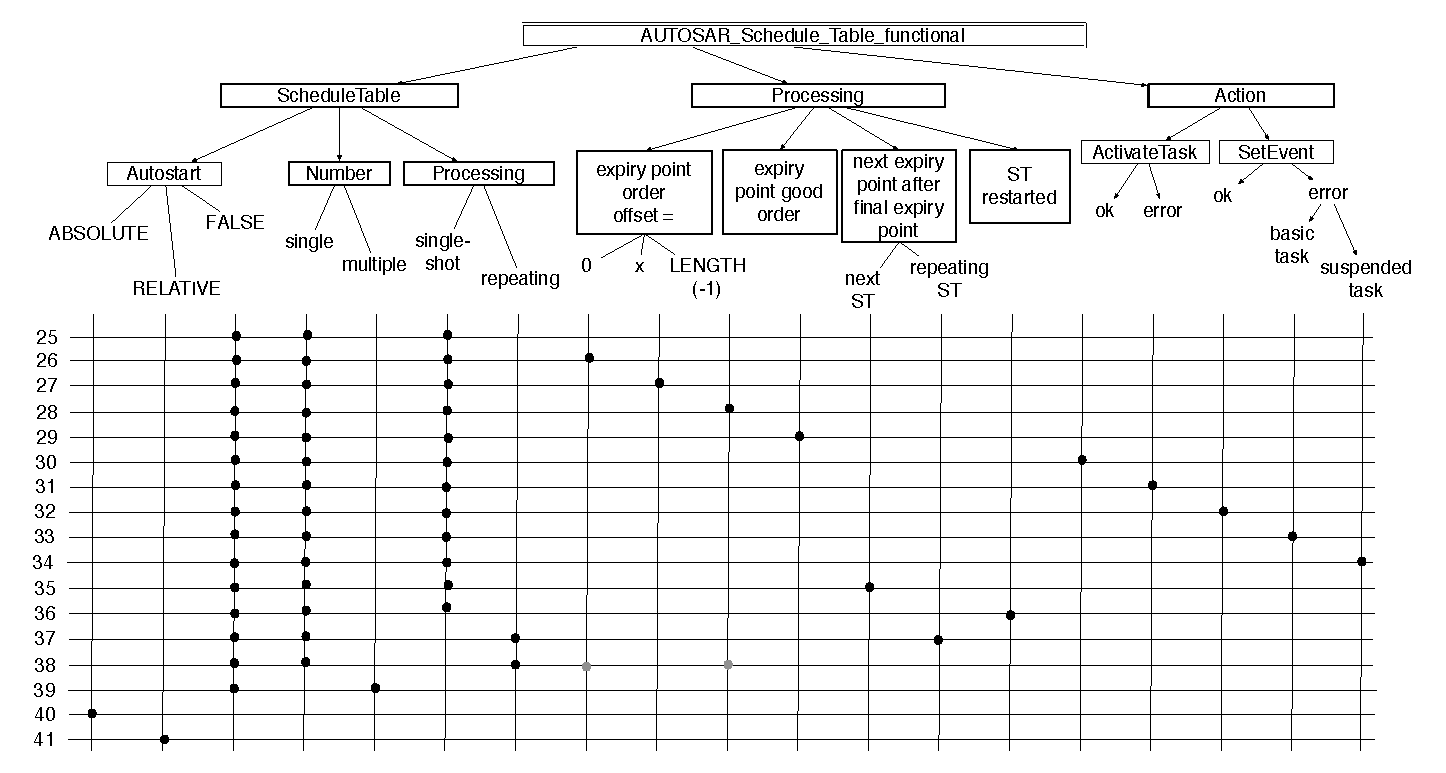
\includegraphics[width=1\textwidth]{graphics/AUTOSAR_Schedule_Table_functional.pdf}
	\end{figure}

	\begin{figure}[htbp] %  figure placement: here, top, bottom, or page
   		\centering
		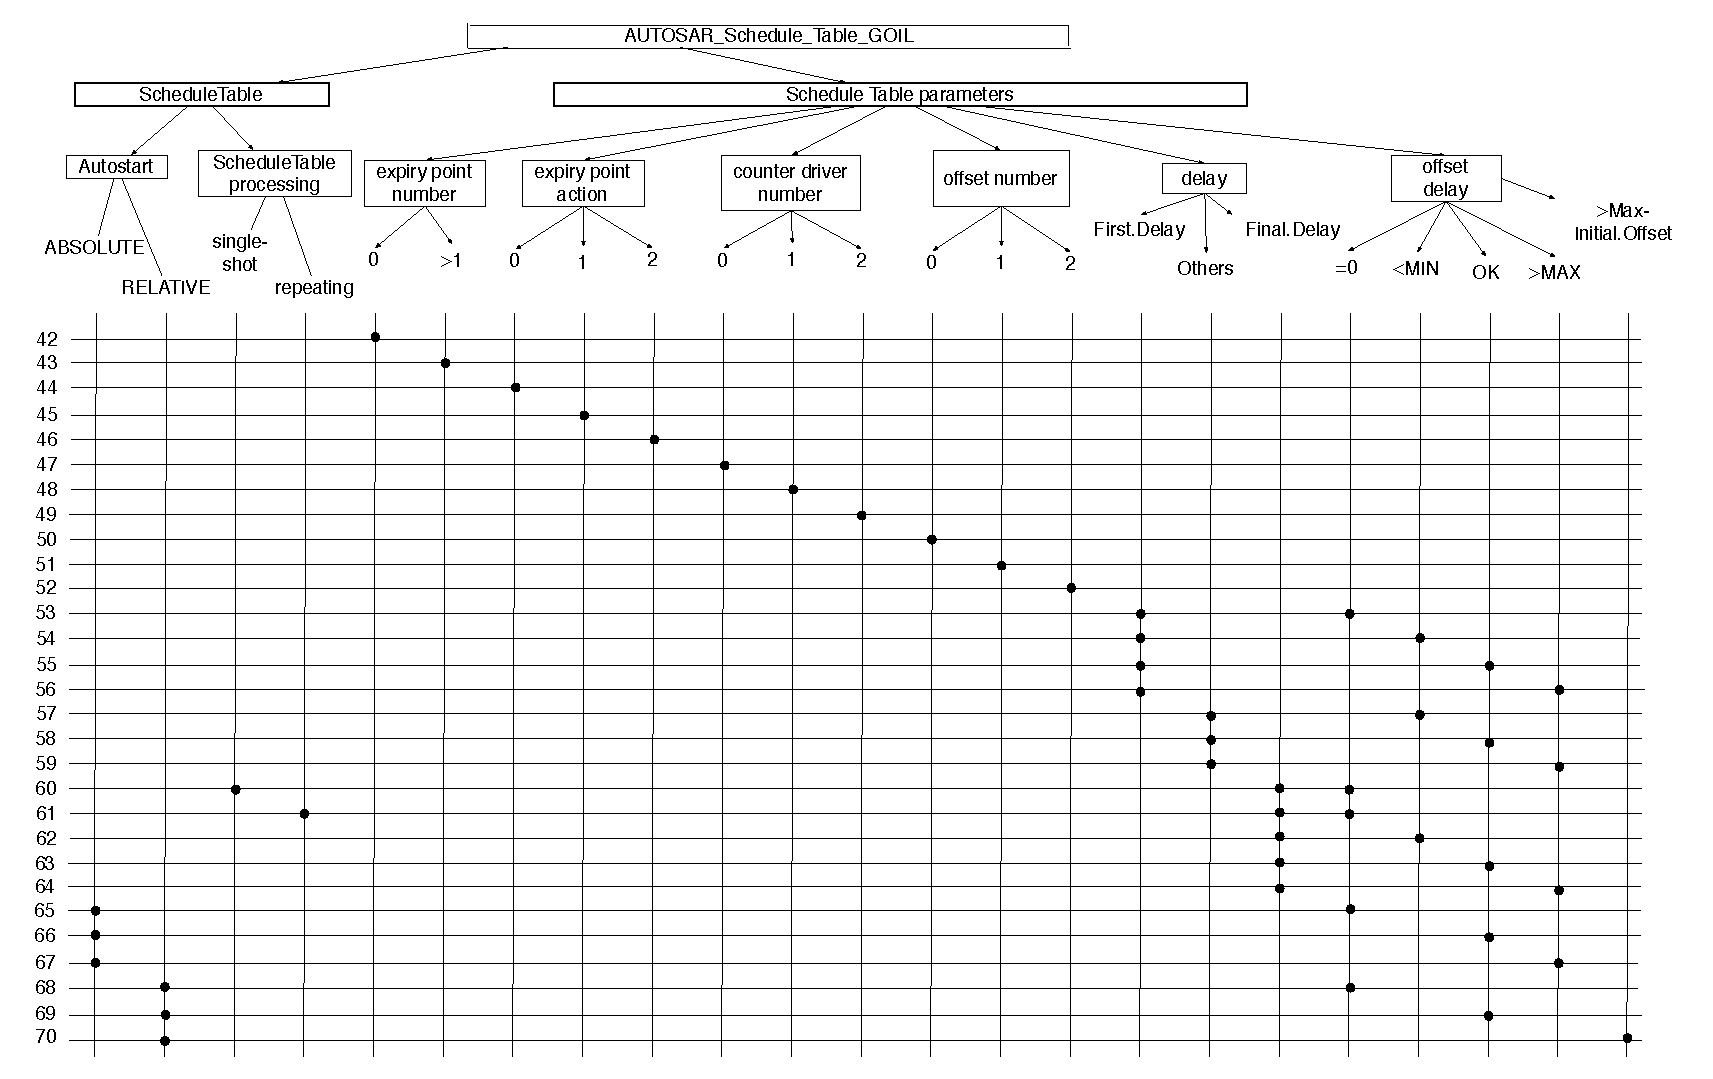
\includegraphics[width=1\textwidth]{graphics/AUTOSAR_Schedule_Table_GOIL.pdf}
	\end{figure}

\setlength{\Lii}{9cm}
\setlength{\Liii}{\textwidth} \addtolength{\Liii}{-\Li} \addtolength{\Liii}{-\Lii} \addtolength{\Liii}{-\Liiiii}

	\begin{supertabular}{|p{\Li}|p{\Lii}|p{\Liii}|p{\Liiiii}|} \hline
	1	& Call StartScheduleTableRel() from task  													&Service returns E\_OK						& OS278, OS358 \\ \hline  
	2 	& Call StartScheduleTableRel() from task with invalid id											& Service returns E\_OS\_ID					& OS275 \\ \hline
	3 	& Call StartScheduleTableRel() from task with $<$offset$>$ value equal to zero						& Service returns E\_OS\_VALUE				& OS332 \\ \hline
	4 	& Call StartScheduleTableRel() from task with $<$offset$>$ $>$ (MAXALLOWEDVALUE - InitialOffset) 		& Service returns E\_OS\_VALUE				& OS276 \\ \hline
	5 	& Call StartScheduleTableRel() from task when schedule table is not in state SCHEDULETABLE\_STOPPED	& Service returns E\_OS\_STATE (in STANDARD and EXTENDED)	& OS277 \\ \hline
	
	6	& Call StartScheduleTableAbs() from task  													&Service returns E\_OK						& OS347, OS351 \\ \hline  
	7 	& Call StartScheduleTableAbs() from task with invalid id											& Service returns E\_OS\_ID					& OS348 \\ \hline
	8 	& Call StartScheduleTableAbs() from task with $<$offset$>$ $>$ (MAXALLOWEDVALUE) 				& Service returns E\_OS\_VALUE				& OS349 \\ \hline
	9 	& Call StartScheduleTableAbs() from task when schedule table is in state SCHEDULETABLE\_STOPPED	& Service returns E\_OS\_STATE (in STANDARD and EXTENDED)	& OS350 \\ \hline
	
	10 	& Call StopScheduleTable() from task 														& Service returns E\_OK						& OS006 OS281, OS453 \\ \hline
	11	& Call StopScheduleTable() from task with invalid id											& Service returns E\_OS\_ID					& OS279 \\ \hline
	12	& Call StopScheduleTable() from task when schedule table is in state SCHEDULETABLE\_STOPPED		& Service returns E\_OS\_NOFUNC	(in STANDARD and EXTENDED) & OS280 \\ \hline
	
	13	& Call NextScheduleTable() from task														& Service returns E\_OK						& OS191, OS284, OS324, OS414 \\ \hline
	14	& Call NextScheduleTable() from task with invalid ScheduleTableID\_From							& Service returns E\_OS\_ID					& OS282 \\ \hline
	15	& Call NextScheduleTable() from task with invalid ScheduleTableID\_To								& Service returns E\_OS\_ID					& OS282 \\ \hline
	16	& Call NextScheduleTable() from task with different schedule table counters							& Service returns E\_OS\_ID					& OS330 \\ \hline
	17	& Call NextScheduleTable() from task when schedule table "from" is in state SCHEDULETABLE\_NEXT		& Service returns E\_OS\_NOFUNC	(in STANDARD and EXTENDED) & OS283 \\ \hline
	18	& Call NextScheduleTable() from task when schedule table "from" is in state SCHEDULETABLE\_STOPPED	& Service returns E\_OS\_NOFUNC (in STANDARD and EXTENDED) & OS283 \\ \hline
	19	& Call NextScheduleTable() from task when schedule table "to" is not in state SCHEDULETABLE\_STOPPED	& Service returns E\_OS\_STATE & OS309 \\ \hline
	
	20 	& Call GetMessageStatus() from task 														& Service returns E\_OK						& OS359 \\ \hline
	21 	& Call GetMessageStatus() from task with invalid id												& Service returns E\_OS\_ID					& OS293 \\ \hline
	22 	& Call GetMessageStatus() from task for a schedule table which waits for the end of the current schedule table	& Service returns E\_OK and SCHEDULETABLE\_NEXT	via $<$ScheduleStatus$>$ & OS353 \\ \hline
	23 	& Call GetMessageStatus() from task for a schedule table which is not started						 	& Service returns E\_OK and SCHEDULETABLE\_STOPPED	via $<$ScheduleStatus$>$	& OS289 \\ \hline
	24 	& Call GetMessageStatus() from task for a schedule table which is started						 	& Service returns E\_OK and SCHEDULETABLE\_RUNNING	via $<$ScheduleStatus$>$	& OS291 \\ \hline
	
	25	& If single-shot ST, stop the schedule table Final Delay ticks after the Final Expiry Point is processed		& & OS009	\\ \hline
	26	& If single-shot ST, an expiry point can be set to offset=0											& & OS002 \\ \hline
	27	& The schedule table has to be processed from the InitialExpiryPoint to the FinalExpiryPoint in order of increasing offset 		& & OS002, OS410 \\ \hline
	28 	& If single-shot ST, an expiry point can be set to offset=LENGTH									& & OS002 \\ \hline
	29	& If single-shot ST, The OS shall process all task activations on an expiry point first and then set events		& & OS412 \\ \hline
	30	& Action of a ST results in a ActivateTask														& & \\ \hline
	31	& Action of a ST results in a ActivateTask and and overflow of Activation occurs. 						& ErrorHook is launched & \\ \hline	
	32	& Action of a ST results in a SetEvent														& & \\ \hline
	33	& Action of a ST results in a SetEvent on a basic task.				 							& error : An action can't set an Event to a basic task (Task t1 is a basic task).	& \\ \hline	
	34	& Action of a ST results in a SetEvent on a suspended task. 										& ErrorHook is launched & \\ \hline	
	35 	& If single-shot ST, Intial expiry point of a 'nexted' ST shall be launched at Final Expiry point + Final Delay + Initial Expiry point (as there's a "finalize" expiry point, this test case as to check when Initial Expiry point is different AND equal to zero.)	& & OS414 \\ \hline
	36 	& A ST restarts from the begging (offset=0)													& & OS428 \\ \hline
	37	& If repeating ST, Initial Expiry Point shall be launched at Final Expiry Point + Final Delay + Initial Offset 		& & OS194 \\ \hline
	38	& If repeating ST, an expiry point can be set to offset=0 and at offset=LENGTH-1						& &  OS002 \\ \hline
	39	& Multiple ST are allowed																	& & OS007 \\ \hline
	40 	& A ST can be autostarted with ABSOLUTE mode. $<$OFFSET$>$ should be in the range MINCYCLE..MAXALLOWEDVALUE OR equal to 0	& & OsSchedule-TableAutostart \\ \hline
	41 	& A ST can be autostarted with RELATIVE mode. $<$START$>$ should be in the range MINCYCLE..MAXALLOWEDVALUE					& & OsSchedule-TableAutostart \\ \hline
	
	42	& No Expiry point in a schedule table														& error : no EXPIRY\_POINT found for SCHEDULETABLE X	& OS401 \\ \hline
	43 	& One or several expiry points in a schedule table												& 											& OS401 \\ \hline
	44	& No Action in an expiry point 																& error : no ACTION found for EXPIRY\_POINT Y		& OS407 \\ \hline
	45	& One action in an expiry point																& 											& OS402, OS403 \\ \hline
	46	& Several actions in an expiry point															& 											& OS407 \\ \hline
	47	& No counter in a schedule table															& error : Counter is not defined in X					& OS409 \\ \hline
	48	& One counter in a schedule table															& 											& OS409 \\ \hline
	49	& Several counters in a schedule table														& error : COUNTER attribute already defined for Schedule Table X 	& OS409 \\ \hline
	50	& No offset in an expiry point																& error : OFFSET is missing for expiry point Y			& OS404 \\ \hline
	51	& One offset in an expiry point																& 											& OS442 \\ \hline
	52	& Several offsets in an expiry point															& error : OFFSET Redefinition						& OS442 \\ \hline
	53 	& First.Delay is equal to 0																	& 											& OS443 \\ \hline
	54 	& First.Delay is lower than MINCYCLE														& error : OFFSET of first expiry point is lower than MINCYCLE of the driving counter and not equal to 0.																													& OS443 \\ \hline 
	55 	& First.Delay is in the range																&											& OS443 \\ \hline 
	56 	& First.Delay is greater than MAXALLOWEDVALUE												& error : OFFSET of first expiry point is greater than MAXALLOWEDVALUE of the driving counter																																& OS443 \\ \hline 
	57 	& Delay between adjacent expiry point is lower than MINCYCLE									& error : Delay between expiry point number A and B is lower than MINCYCLE of the driving counter																															& OS408 \\ \hline 
	58 	& Delay between adjacent expiry point is in the range											&											& OS408 \\ \hline 
	59 	& Delay between adjacent expiry point is greater than MAXALLOWEDVALUE							& error : Delay between expiry point number A and B is greater than MAXALLOWEDVALUE of the driving counter																										& OS408 \\ \hline
	60	& In single-shot, Final.Delay is equal to 0														& 											& OS427 \\ \hline
	61	& In repeating, Final.Delay is equal to 0														& error : Final delay can be equal to 0 only for single-shot schedule table and X is a repeating one																													& OS444 \\ \hline
	62 	& Final.Delay is lower than MINCYCLE														& error : Final delay should be within MINCYCLE and MAXALLOWEDVALUE of the driving counter																															& OS444 \\ \hline 
	63 	& Final.Delay is in the range																&											& OS444 \\ \hline 
	64 	& Final.Delay is greater than MAXALLOWEDVALUE											& error : Final delay should be within MINCYCLE and MAXALLOWEDVALUE of the driving counter																															& OS444 \\ \hline 
	
	65	& In an ABSOLUTE autostarted schedule table, $<$OFFSET$>$ is equal to 0							& 											& \\ \hline
	66	& In an ABSOLUTE autostarted schedule table, $<$OFFSET$>$ is lower than MAXALLOWEDVALUE	 	& 											& \\ \hline
	67	& In an ABSOLUTE autostarted schedule table, $<$OFFSET$>$ is greater than MAXALLOWEDVALUE 		& error : X autostart's offset is greater than MAXALLOWEDVALUE																																					& OS349 \\ \hline
	68	& In an RELATIVE autostarted schedule table, $<$START$>$ is equal to 0							& error : X autostart's offset is equal to 0			 	& OS332 \\ \hline
	69	& In an RELATIVE autostarted schedule table, $<$START$>$ is lower than (MAXALLOWEDVALUE - Initial.Offset)	 	& 									& \\ \hline
	70	& In an RELATIVE autostarted schedule table, $<$START$>$ is greater than (MAXALLOWEDVALUE - Initial.Offset)	& error : X autostart's offset is greater than (MAXALLOWEDVALUE - Initial.Offset)																																& OS276 \\ \hline
	\end{supertabular} \\

	When a schedule table is started, the first expiry point can be set to the "second" value of a counter tick (only with StartScheduleTableAbs) if :
	\begin{itemize}
		\item ($<$start$>$ $>$ current date) AND ($<$start$>$ + FirstDelay - MAX\_ALLOWED\_VALUE) $>$ current date
		\item ($<$start$>$ $<$ current date) AND (($<$start$>$ + FirstDelay) $>$ current date)
	\end{itemize}
	Because of that, more tests has to be done to check that the expiry point is not launched at the first value of the counter but at the "second". In Trampoline, we use a "Bootstrap" to implement the solution. A bit of the schedule table's state is set to '1' when the first expiry point has reached the conditions above. When the time object is launched, we take a look at the state and if the bit is '1', we take out the time object and place it before the current date, setting the bit to '0'. In this way, the expiry point is shifted to the "second" value of the counter. \\
	Moreover, other tests have to check the correct functionning of the sequences when there are only "bootstraped" schedule table on an expiry point, or when there are "bootstraped" and "normal" schedule tabe, whatever the first inserted in the counter's date. \\ 
	The plan below conclues on the schedule table tests. "Date" is the date of the first expiry point. \\

	\begin{figure}[htbp] %  figure placement: here, top, bottom, or page
  		\centering
		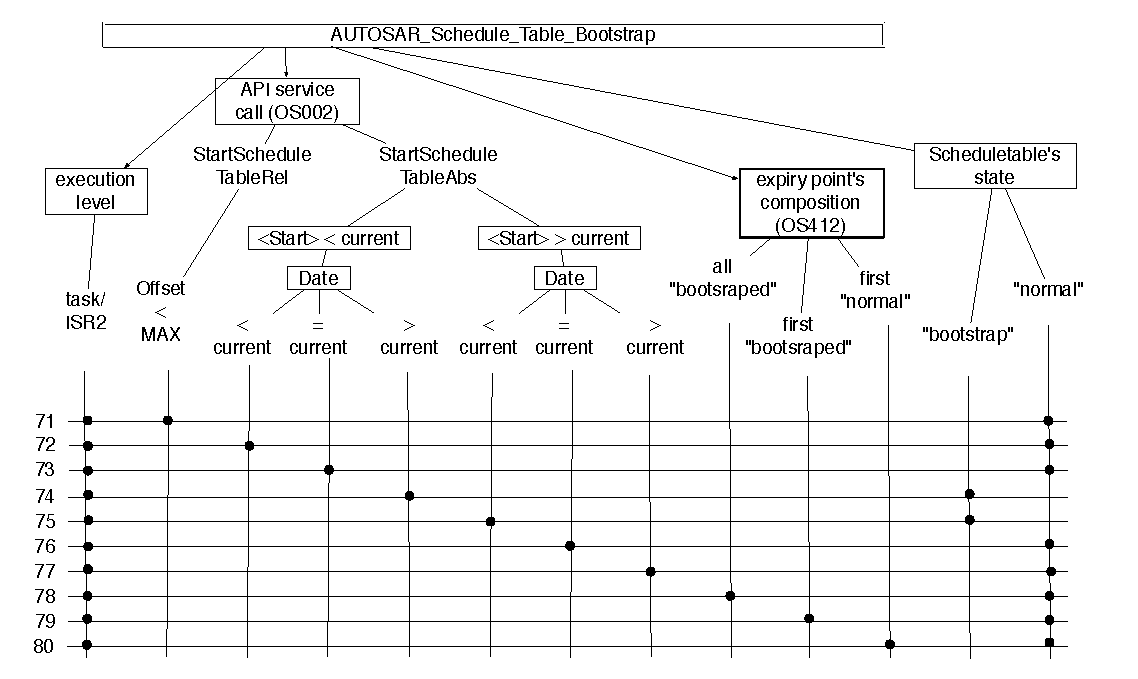
\includegraphics[width=0.85\textwidth]{graphics/AUTOSAR_Schedule_Table_Bootstrap.pdf}
	\end{figure}
	
\setlength{\Lii}{7,5cm}
\setlength{\Liiii}{1cm}
\tablefirsthead{ \hline \rowcolor{lightgray} Test Case No. & Action & Expected Result \\ }
\tablehead{ \hline \rowcolor{lightgray} Test Case No. & Action & Expected Result\\}
\setlength{\Liii}{\textwidth} \addtolength{\Liii}{-\Li} \addtolength{\Liii}{-\Lii}

	\begin{supertabular}{|p{\Li}|p{\Lii}|p{\Liii}|} \hline
	71	& Call StartScheduleTableRel() from task. Offset is lower than max allowed value of the counter.					& Service returns E\_OK				 \\ \hline  
	72 	& Call StartScheduleTableAbs() from task. $<$Start$>$ and Date are lower than current date.						& Service returns E\_OK				  \\ \hline
	73 	& Call StartScheduleTableAbs() from task. $<$Start$>$ is lower than current date and Date is equal to current date.	& Service returns E\_OK				  \\ \hline
	74 	& Call StartScheduleTableAbs() from task. $<$Start$>$ is lower than current date and Date is greater than current date.	& Service returns E\_OK. The schedule table is set to a "bootstrap" one.  \\ \hline
	75 	& Call StartScheduleTableAbs() from task. $<$Start$>$ is greater than current date and Date is lower than current date. & Service returns E\_OK				 \\ \hline
	76 	& Call StartScheduleTableAbs() from task. $<$Start$>$ is greater than current date and Date is equal to current date.	& Service returns E\_OK				 \\ \hline
	77 	& Call StartScheduleTableAbs() from task. $<$Start$>$ and Date are greater than current date.					& Service returns E\_OK.  The schedule table is set to a "bootstrap" one.  \\ \hline
	78	& Set several "bootstraped" schedule table to a same date 												& Expiry points stay in the list and schedule table state becomes "normal"\\ \hline
	79	& Set several "bootstraped" and "normal" schedule table to a same date. A "bootstrap" schedule table is inserted first in the list. 	& Expiry points which was "bootstraped" stay in the list and there schedule table state becomes "normal". Expiry point which was "normal" are taken out of the list. \\ \hline
	80	& Set several "bootstraped" and "normal" schedule table to a same date. A "normal" schedule table is inserted first in the list. 		& Expiry points which was "bootstraped" stay in the list and there schedule table state becomes "normal". Expiry point which was "normal" are taken out of the list. \\ \hline
	\end{supertabular} \\


	% AUTOSAR - SCHEDULE TABLE SYNCHRONIZATION %
	\subsection{AUTOSAR - Schedule Table Synchronisation}
	OS Requirements : 013, 199, 201, 206, 227, 278, 290, 291, 300, 323, 351, 354, 362, (363), 387, 388, 389, 417, 418, 419, 420, 421, 422, 429, 430, 434, 435, 452, 454, 455, 456, 457, 458 \\
	OS462 and OS463 can't be tested. \\
	OS Requirements  415, 416, 429, 430, 431, 436, 437, 438 are GOIL test cases (Test cases 38 to 60).\\
	
	\begin{figure}[htbp] %  figure placement: here, top, bottom, or page
  		\centering
		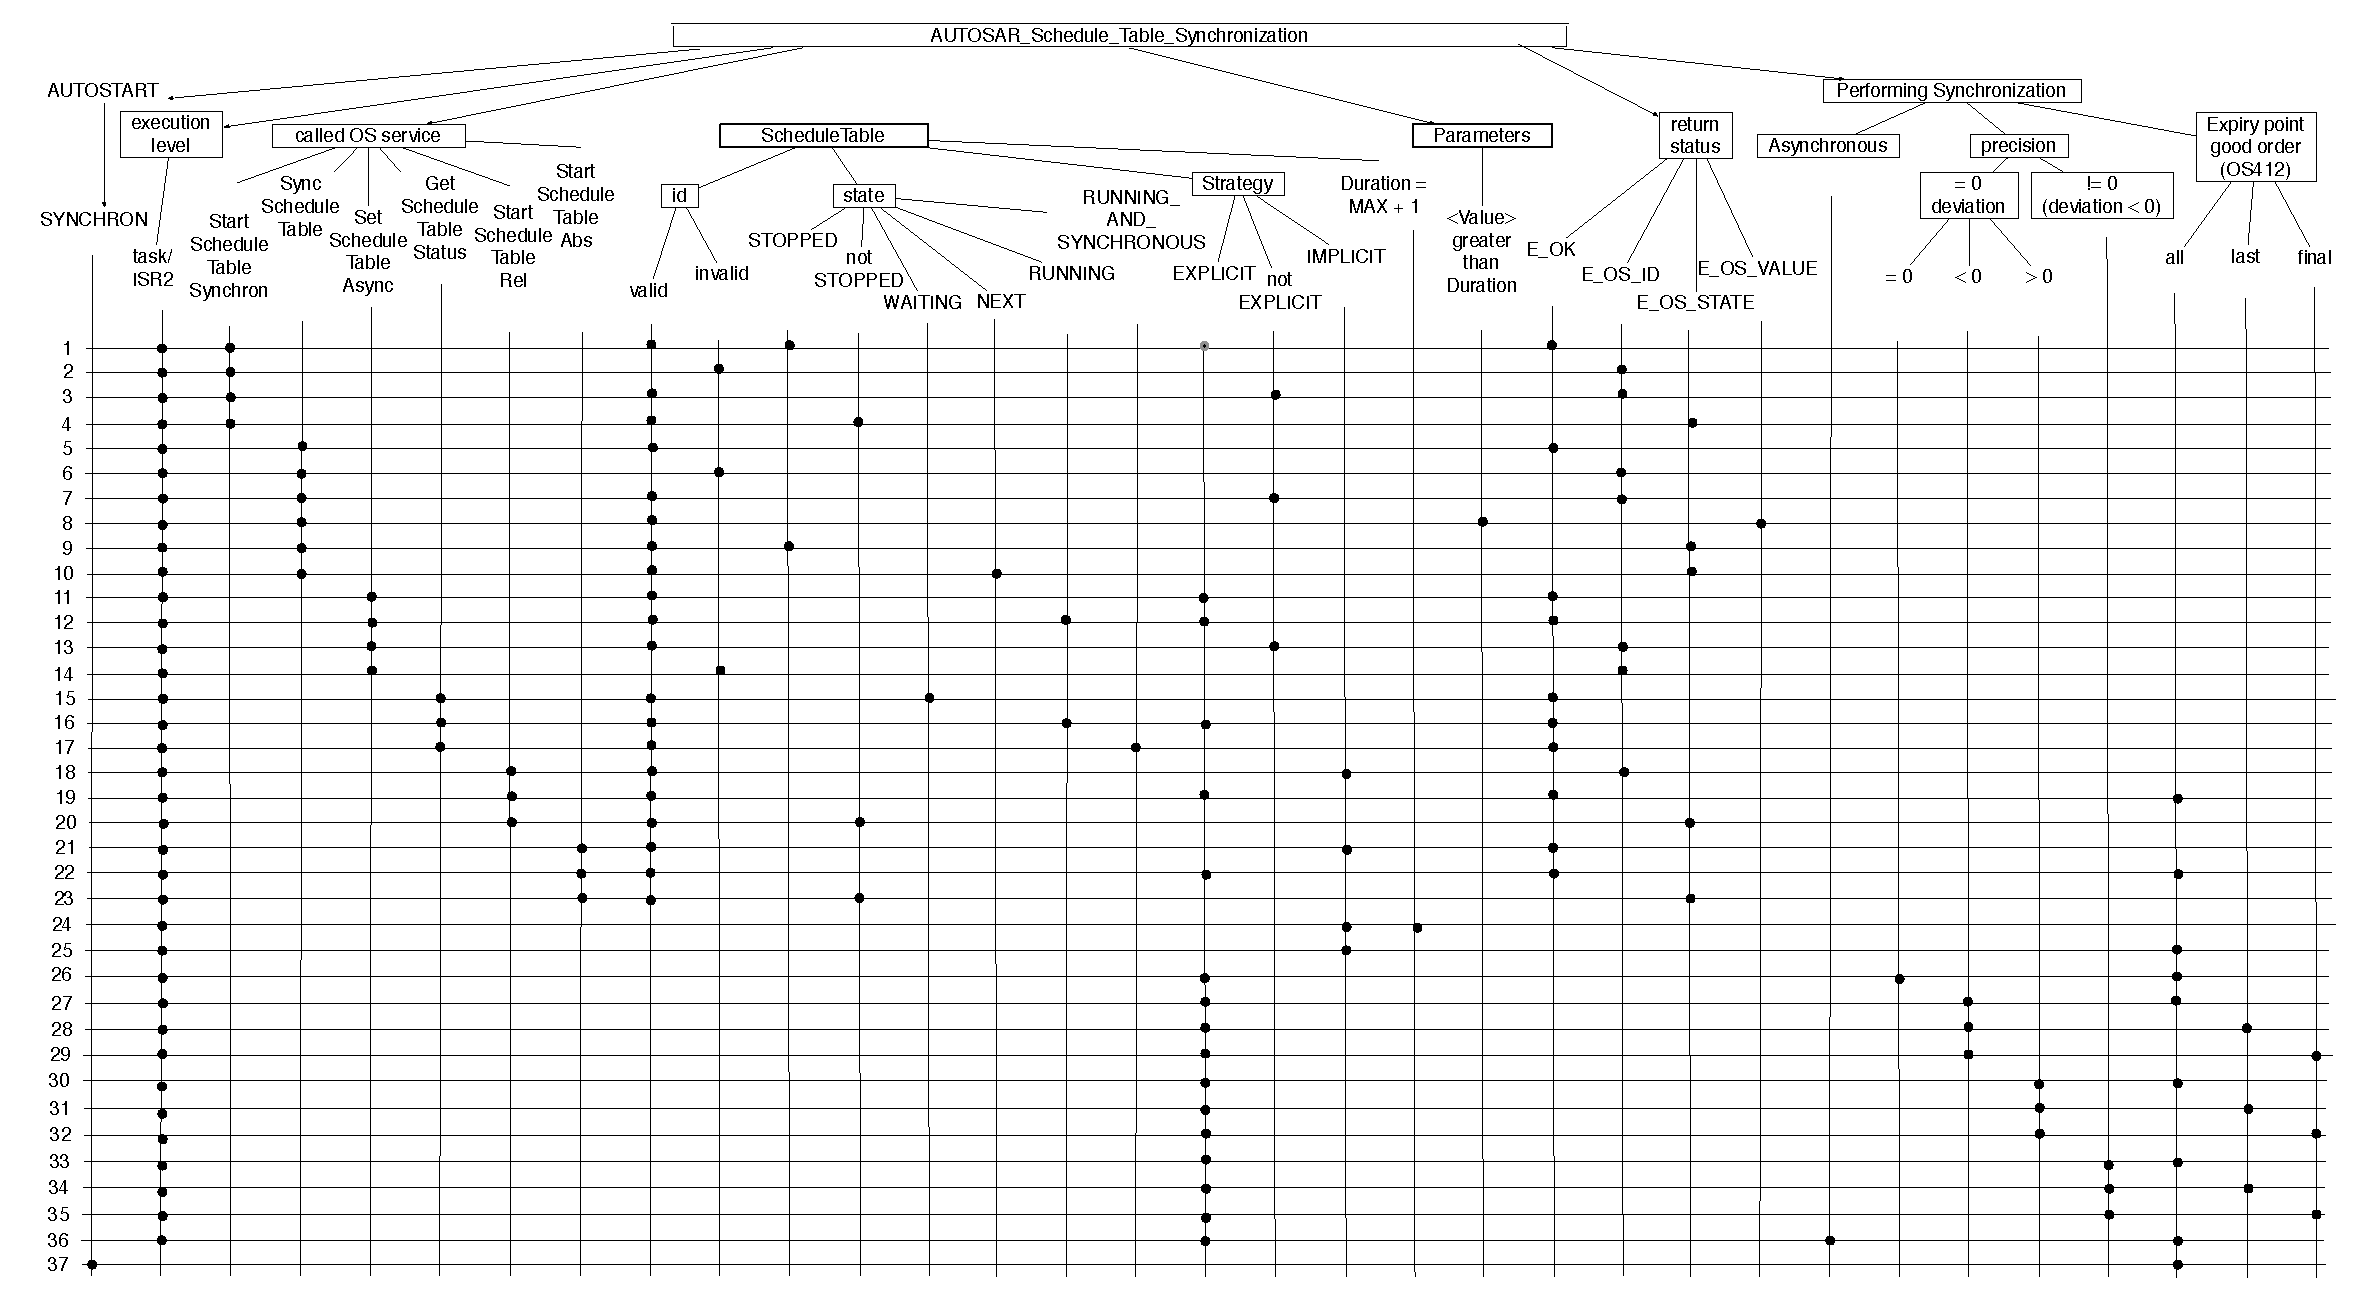
\includegraphics[width=1\textheight, angle=90]{graphics/AUTOSAR_Schedule_Table_Synchronization.pdf}
	\end{figure}
	
	\begin{figure}[htbp] %  figure placement: here, top, bottom, or page
  		\centering
		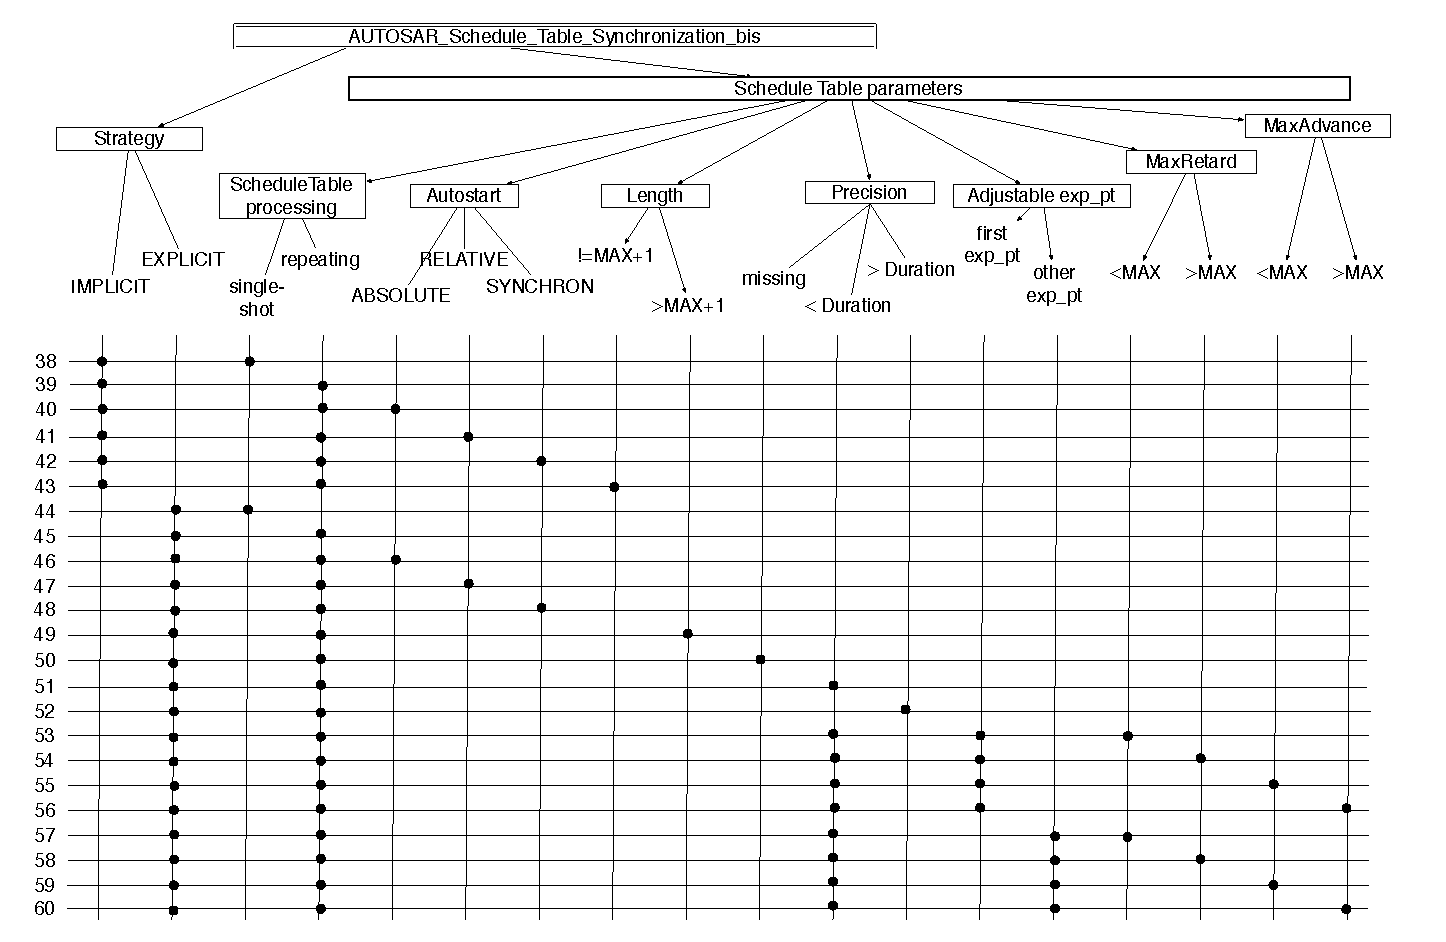
\includegraphics[width=1\textwidth]{graphics/AUTOSAR_Schedule_Table_Synchronization_bis.pdf}
	\end{figure}
	
\setlength{\Lii}{7cm}
\setlength{\Liiii}{2,5cm}
\setlength{\Liii}{\textwidth} \addtolength{\Liii}{-\Li} \addtolength{\Liii}{-\Lii} \addtolength{\Liii}{-\Liiii}
\tablefirsthead{ \hline \rowcolor{lightgray} Test Case No. & Action & Expected Result  & OS Requirements\\ }
\tablehead{ \hline \rowcolor{lightgray} Test Case No. & Action & Expected Result & OS Requirements \\}
	
	\begin{supertabular}{|p{\Li}|p{\Lii}|p{\Liii}|p{\Liiii}|} \hline
	1	& Call StartScheduleTableSynchron() from task/ISR2. The state of the schedule table is equal to SCHEDULETABLE\_STOPPED		&  Service returns E\_OK, the state is set to SCHEDULETABLE\_WAITING				 																											& OS389, OS435 \\ \hline
	2	& Call StartScheduleTableSynchron() from task/ISR2 with invalid id														&  Service returns E\_OS\_ID			& OS387 \\ \hline  
	3	& Call StartScheduleTableSynchron() from task/ISR2. The schedule table is not explicitly synchronized							&  Service returns E\_OS\_ID			& OS387 \\ \hline  
	4	& Call StartScheduleTableSynchron() from task/ISR2. The state of the schedule table is not equal to SCHEDULETABLE\_STOPPED	&  Service returns E\_OS\_STATE (in STANDARD and EXTENDED)		& OS388 \\ \hline  
	5	& Call SyncScheduleTable() from task/ISR2. 																		&  Service returns E\_OK, the processing of the schedule table is started							 																									& OS013, OS457, OS199, OS201\\ \hline  
	6	& Call SyncScheduleTable() from task/ISR2 with invalid id															&  Service returns E\_OS\_ID			& OS454 \\ \hline  
	7	& Call SyncScheduleTable() from task/ISR2. The schedule table is not explicitly synchronized									&  Service returns E\_OS\_ID			& OS454 \\ \hline  
	8	& Call SyncScheduleTable() from task/ISR2. The $<$value$>$ is greater than OSScheduleTableDuration						&  Service returns E\_OS\_VALUE		& OS455 \\ \hline  
	9	& Call SyncScheduleTable() from task/ISR2. The state of the schedule table is equal to SCHEDULETABLE\_STOPPED				&  Service returns E\_OS\_STATE		& OS456 \\ \hline
	10	& Call SyncScheduleTable() from task/ISR2. The state of the schedule table is equal to SCHEDULETABLE\_NEXT				&  Service returns E\_OS\_STATE		& OS456 \\ \hline
	11	& Call SetScheduleTableAsync() from task/ISR2. The schedule table is explicitly synchronized								&  Service returns E\_OK, the state is set to SCHEDULETABLE\_RUNNING 			 																											& OS300 \\ \hline  
	12	& Call SetScheduleTableAsync() from task/ISR2. The schedule table is explicitly synchronized and the state of the schedule table is equal to SCHEDULETABLE\_RUNNING	&  Service returns E\_OK, the synchronisation is stopped but expiry point are still processed																					& OS362, OS323, OS422 \\ \hline  
	13	& Call SetScheduleTableAsync() from task/ISR2. The schedule table's strategy is not equal to EXPLICIT							&  Service returns E\_OS\_ID			& OS458 \\ \hline  
	14	& Call SetScheduleTableAsync() from task/ISR2 with invalid id														&  Service returns E\_OS\_ID			& OS458 \\ \hline  
	15	& Call GetScheduleTableStatus() from task/ISR2. The schedule table is EXCPLICIT and no synchronisation count was provided		& Service returns E\_OK and SCHEDULETABLE\_WAITING via $<$ScheduleStatus$>$																													& OS354, OS227 \\ \hline
	16	& Call GetScheduleTableStatus() from task/ISR2. The schedule table is started AND NOT synchronous							& Service returns E\_OK and SCHEDULETABLE\_RUNNING via $<$ScheduleStatus$>$																													& OS291 \\ \hline
	17	& Call GetScheduleTableStatus() from task/ISR2. The schedule table is started AND synchronous (deviation in the precision interval)	& Service returns E\_OK and SCHEDULETABLE\_RUNNING\_AND\_SYNCHRONOUS via $<$ScheduleStatus$>$																								& OS290 \\ \hline
	18	& Call StartScheduleTableRel() from task/ISR2. The schedule table's strategy is IMPLICIT									& Service returns E\_OS\_ID			& OS452, OS430 \\ \hline  
	19	& Call StartScheduleTableRel() from task/ISR2. The schedule table's strategy is EXPLICIT									& Service returns E\_OK, the processing of the schedule table is started and the state is SCHEDULETABLE\_RUNNING																									& OS278, OS434 \\ \hline  
	20	& Call StartScheduleTableRel() from task/ISR2. The schedule table's strategy is EXPLICIT and its state is not stopped				& Service returns E\_OS\_STATE		& OS277 \\ \hline  
	
	21	& Call StartScheduleTableAbs() from task/ISR2. The schedule table's strategy is IMPLICIT									& Service returns E\_OK, the processing of the schedule table is started and the state is SCHEDULETABLE\_RUNNING																									& OS351 \\ \hline  
	22	& Call StartScheduleTableAbs() from task/ISR2. The schedule table's strategy is EXPLICIT									& Service returns E\_OK, the processing of the schedule table is started and the state is SCHEDULETABLE\_RUNNING																									& OS351, OS434 \\ \hline  
	
	23	& Call StartScheduleTableAbs() from task/ISR2. The schedule table's strategy is EXPLICIT and its state is not stopped				& Service returns E\_OS\_STATE		& OS350 \\ \hline  
	
	24 	& An IMPLICIT schedule table shall have a period equal to ( MAX\_ALLOWED\_VALUE + 1 ) of its counter						& 								& OS429 \\ \hline 
	25	& An IMPLICIT schedule table is always synchronized.																& Next expiry point is inserted in the list	&  \\ \hline
	
	26	& No synchronisation with deviation equal to 0																		& Next expiry point is inserted in the list	& OS389, OS201 \\ \hline
	27	& Performing synchronisation with precision equal to 0 and deviation less than 0. Check expiry point good order					& According to deviation and MaxRetard, Next expiry point is inserted in the list																																& OS206, OS417, OS420 \\ \hline
	28	& Performing synchronisation with precision equal to 0 and deviation less than 0. Check expiry point good order on last expiry point	& According to deviation and MaxRetard, First expiry point is adjusted and if comes before Final expiry point, Final expiry point is adjuted to the same offset of First expiry point and inserted in the list and First expiry point offset becomes 0	& OS420\\ \hline
	29	& Performing synchronisation with precision equal to 0 and deviation less than 0. Check expiry point good order on final expiry point	& According to deviation and MaxRetard, First expiry point is launched now if First.Delay equal to 0, otherwise if only one expiry point in the ST (the final one), adjust the Final expiry point, insert it in the list and First expiry point offset becomes 0 otherwise is adjusted and inserted in the list 																														& OS420\\ \hline
	30	& Performing synchronisation with precision equal to 0 and deviation greater than 0. Check expiry point good order				& According to deviation and MaxAdvance, Next expiry point is inserted in the list																																& OS421 \\ \hline
	31	& Performing synchronisation with precision equal to 0 and deviation greater than 0. Check expiry point good order on last expiry point	& According to deviation and MaxAdvance, First expiry point is adjusted and Final expiry point is  inserted in the list																									& OS421 \\ \hline
	32	& Performing synchronisation with precision equal to 0 and deviation greater than 0. Check expiry point good order on final expiry point	& According to deviation and MaxAdvance, First expiry point is launched now if First.Delay equal to 0, otherwise is adjusted and inserted in the list 																		& OS421 \\ \hline
	33	& Performing synchronisation with precision different than 0 and deviation less than 0. Check expiry point good order				& According to deviation, precision and MaxRetard, Next expiry point is inserted in the list																														& OS418, OS419 \\ \hline
	34	& Performing synchronisation with precision different than 0 and deviation less than 0. Check expiry point good order on last expiry point	& According to deviation, precision and MaxRetard, First expiry point is adjusted and if comes before Final expiry point, Final expiry point is adjuted to the same offset of First expiry point and inserted in the list and First expiry point offset becomes 0																																		& OS418, OS419 \\ \hline
	35	& Performing synchronisation with precision different than 0 and deviation less than 0. Check expiry point good order on final expiry point	& According to deviation, precision and MaxRetard, First expiry point is launched now if First.Delay equal to 0, otherwise if only one expiry point in the ST (the final one), adjust the Final expiry point, insert it in the list and First expiry point offset becomes 0 otherwise is adjusted and inserted in the list 																									& OS418, OS419 \\ \hline
	36	& No synchronisation if schedule table asynchronous																& Next expiry point is inserted in the list	& OS362, OS323 \\ \hline 
	37 	& A schedule table can be autostarted with SYNCHRON mode														& The state is SCHEDULETABLE\_WAITING 	& OsSchedule-TableAutostart \\ \hline
	38 	& IMPLICIT schedule table is single-shot 								& A synchronized schedule table shall be repeating otherwise, synchronisation can't be done.	& \\ \hline
	39 	& IMPLICIT schedule table is repeating		 						&  																			& \\ \hline
	40 	& IMPLICIT schedule table autostarts in ABSOLUTE mode				&  																			& \\ \hline
	41 	& IMPLICIT schedule table autostarts in RELATIVE mode					& An IMPLICIT schedule table should be started in Absolute mode only						& OS430  \\ \hline
	42 	& IMPLICIT schedule table autostarts in SYNCHRON mode				& An IMPLICIT schedule table should be started in Absolute mode only						& OS430 \\ \hline
	43 	& IMPLICIT schedule table duration is different to MAXALLOWEDVALUE + 1	& An IMPLICIT schedule table should have a duration equal to OSMAXALLOWEDVALUE + 1 of its counter.				& OS429 \\ \hline
	44 	& EXPLICIT schedule table is single-shot								& A synchronized schedule table shall be repeating otherwise, synchronisation can't be done.	& \\ \hline
	45 	& EXPLICIT schedule table is repeating		 						&																			& \\ \hline
	46 	& EXPLICIT schedule table autostarts in ABSOLUTE mode				&																			& \\ \hline
	47 	& EXPLICIT schedule table autostarts in RELATIVE mode				&																			& \\ \hline
	48 	& EXPLICIT schedule table autostarts in SYNCHRON mode				&																			& \\ \hline
	49 	& EXPLICIT schedule table duration is greater than MAXALLOWEDVALUE + 1	& An EXPLICIT schedule table shouldn't have a duration greater than OSMAXALLOWEVALUE + 1 of its counter.				& OS431 \\ \hline	
	50 	& EXPLICIT schedule table precision missing							& PRECISION attribute is missing													& \\ \hline
	51 	& EXPLICIT schedule table precision lower than duration					& 																			& \\ \hline
	52 	& EXPLICIT schedule table precision greater than duration				& An explicit schedule table shall have a precision in the range 0 to duration.					& OS438 \\ \hline
	53 	& In the first expiry point of an EXPLICIT schedule table, MaxRetard is lower than the maximum value allowed	& 												& \\ \hline
	54 	& In the first expiry point of an EXPLICIT schedule table, MaxRetard is greater than the maximum value allowed	& In first expiry point, MaxRetard should be inferior to the previous delay minus MINCYCLE of the counter.																													& OS415, OS436 \\ \hline
	55 	& In the first expiry point of an EXPLICIT schedule table, MaxAdvance is lower than the maximum value allowed	& 												&  \\ \hline
	56 	& In the first expiry point of an EXPLICIT schedule table, MaxAdvance is greater than the maximum value allowed	& In first expiry point, MaxAdvance should be inferior to duration minus the first delay.																																& OS416, OS437 \\ \hline
	57 	& In an expiry point of an EXPLICIT schedule table, MaxRetard is lower than the maximum value allowed		& 												& \\ \hline
	58 	& In an expiry point of an EXPLICIT schedule table, MaxRetard is greater than the maximum value allowed		& In expiry point at offset X, MaxRetard should be inferior to the previous delay minus MINCYCLE of the counter.																										& OS415, OS436 \\ \hline
	59 	& In an expiry point of an EXPLICIT schedule table, MaxAdvance is lower than the maximum value allowed		& 												& \\ \hline
	60 	& In an expiry point of an EXPLICIT schedule table, MaxAdvance is greater than the maximum value allowed		& In expiry point at offset X, MaxAdvance should be inferior to duration minus the previous delay.																														& OS416, OS4337 \\ \hline
	\end{supertabular} \\
	
	% AUTOSAR - SERVICE CALLS ON OBJECTS IN DIFFERENT OS-APPLCIATION %
	\subsection{AUTOSAR - OS-Application}
	
	\subsubsection{API Service Calls for OS objects}
	OS Requirements : 016, 017, 256, 258, 261, 262, 271, 272, 273, 274, 287, 318, 319, 346, 423, 445, 447, 450, 459\\
	OS288* is in the sequence which test all the API service calls from wrong context.\\
	
	\begin{figure}[htbp] %  figure placement: here, top, bottom, or page
  		\centering
		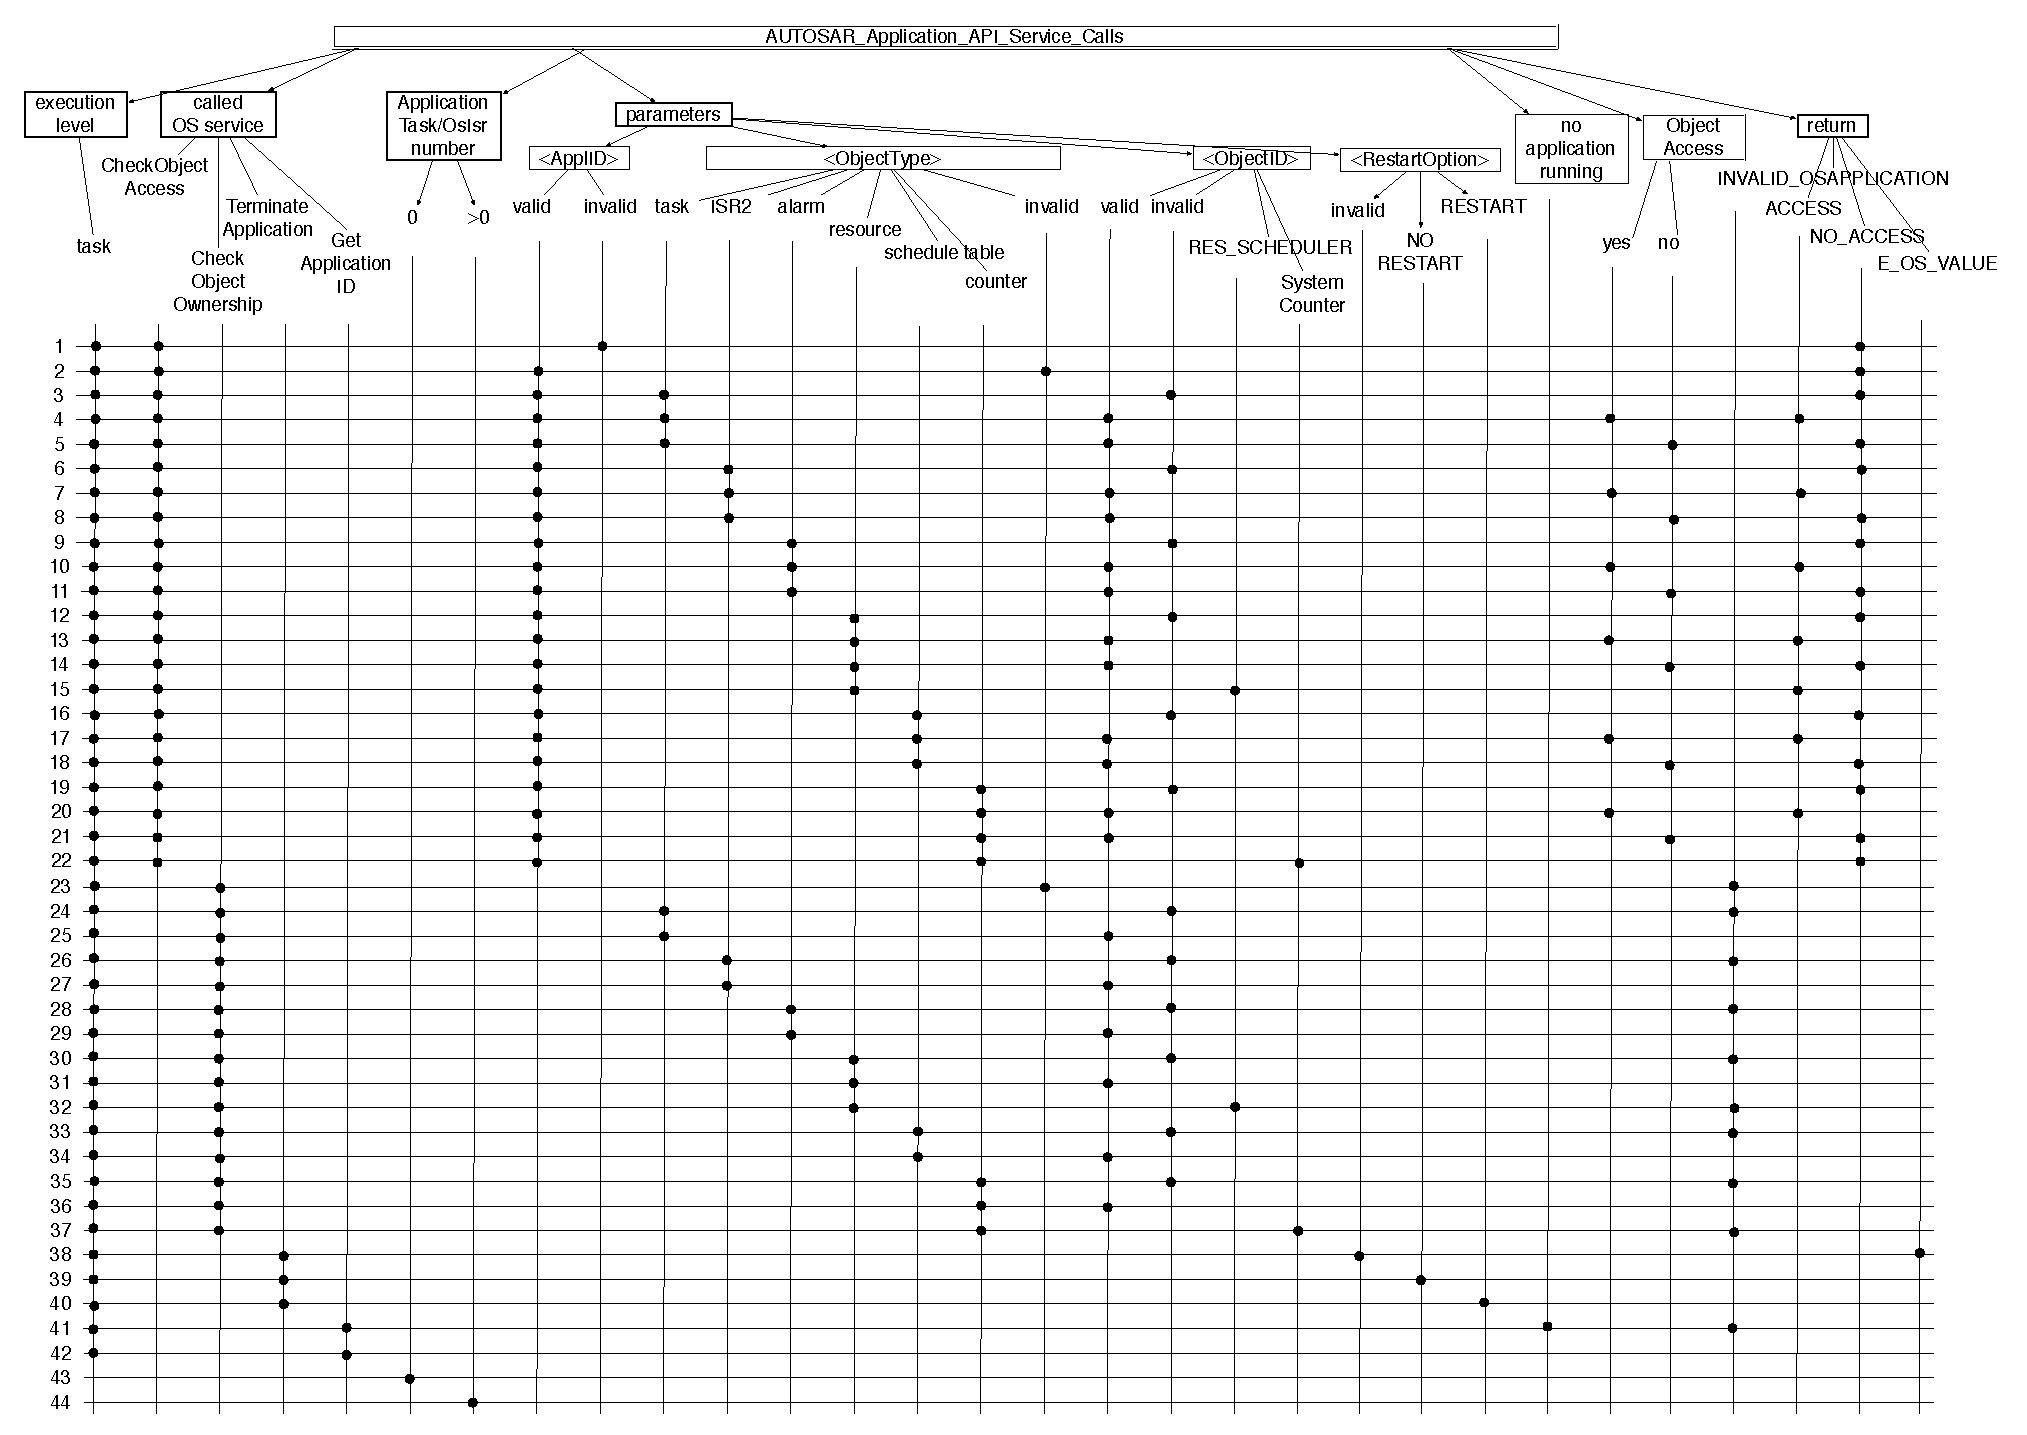
\includegraphics[width=1\textheight, angle=90]{graphics/AUTOSAR_Application_API_Service_Calls.pdf}
	\end{figure}

	\begin{supertabular}{|p{\Li}|p{\Lii}|p{\Liii}|p{\Liiii}|} \hline
	1	& Call CheckObjectAccess() with $<$AppID$>$ invalid 												& Service returns NO\_ACCESS 			& OS423 \\ \hline
	2	& Call CheckObjectAccess() with $<$ObjectType$>$ invalid											& Service returns NO\_ACCESS 			& OS423 \\ \hline
	3	& Call CheckObjectAccess() for a task object type with $<$ObjectID$>$ invalid							& Service returns NO\_ACCESS 			& OS423 \\ \hline
	4	& Call CheckObjectAccess() for a task object type, \textit{running} task/ISR2 has access to the object 			& Service returns ACCESS	 			& OS256, OS271, OS450 \\ \hline
	5	& Call CheckObjectAccess() for a task object type, \textit{running} task/ISR2 has NO access to the object			& Service returns NO\_ACCESS	 		& OS272 \\ \hline
	6	& Call CheckObjectAccess() for an ISR2 object type with $<$ObjectID$>$ invalid							& Service returns NO\_ACCESS 			&  \\ \hline
	7	& Call CheckObjectAccess() for an ISR2 object type, \textit{running} task/ISR2 has access to the object 			& Service returns ACCESS	 			&  \\ \hline
	8	& Call CheckObjectAccess() for an ISR2 object type, \textit{running} task/ISR2 has NO access to the object		& Service returns NO\_ACCESS	 		&  \\ \hline
	9	& Call CheckObjectAccess() for an alarm object type with $<$ObjectID$>$ invalid							& Service returns NO\_ACCESS 			&  \\ \hline
	10	& Call CheckObjectAccess() for an alarm object type, \textit{running} task/ISR2 has access to the object	 		& Service returns ACCESS	 			&  \\ \hline
	11	& Call CheckObjectAccess() for an alarm object type, \textit{running} task/ISR2 has NO access to the object		& Service returns NO\_ACCESS	 		&  \\ \hline
	12	& Call CheckObjectAccess() for a resource object type with $<$ObjectID$>$ invalid						& Service returns NO\_ACCESS 			&  \\ \hline
	13	& Call CheckObjectAccess() for a resource object type, \textit{running} task/ISR2 has access to the object 		& Service returns ACCESS	 			&  \\ \hline
	14	& Call CheckObjectAccess() for a resource object type, \textit{running} task/ISR2 has NO access to the object		& Service returns NO\_ACCESS	 		&  \\ \hline
	15	& Call CheckObjectAccess() for a resource object type (RES\_SCHEDULER)								& Service returns ACCESS	 			& OS318 \\ \hline
	16	& Call CheckObjectAccess() for a schedule table object type with $<$ObjectID$>$ invalid					& Service returns NO\_ACCESS 			&  \\ \hline
	17	& Call CheckObjectAccess() for a schedule table object type, \textit{running} task/ISR2 has access to the object 	& Service returns ACCESS	 			&  \\ \hline
	18	& Call CheckObjectAccess() for a schedule table object type, \textit{running} task/ISR2 has NO access to the object	& Service returns NO\_ACCESS 		&  \\ \hline
	19	& Call CheckObjectAccess() for a counter object type with $<$ObjectID$>$ invalid							& Service returns NO\_ACCESS 			&  \\ \hline
	20	& Call CheckObjectAccess() for a counter object type, \textit{running} task/ISR2 has access to the object 		& Service returns ACCESS	 			&  \\ \hline
	21	& Call CheckObjectAccess() for a counter object type, \textit{running} task/ISR2 has NO access to the object		& Service returns NO\_ACCESS	 		&  \\ \hline
	22	& Call CheckObjectAccess() for a counter object type (SystemCounter)									& Service returns NO\_ACCESS 			&  \\ \hline
	23	& Call CheckObjectOwnerShip() with $<$ObjectType$>$ invalid										& Service returns INVALID\_OSAPPLICATION	& OS274, OS017 \\ \hline
	24	& Call CheckObjectOwnerShip() for a task object type with $<$ObjectID$>$ invalid							& Service returns INVALID\_OSAPPLICATION	& OS274 \\ \hline
	25	& Call CheckObjectOwnerShip() for a task object type												& Service returns the identifier of the OS-Application to which the object belongs			& OS273 \\ \hline
	26	& Call CheckObjectOwnerShip() for an ISR2 object type with $<$ObjectID$>$ invalid						& Service returns INVALID\_OSAPPLICATION	& \\ \hline
	27	& Call CheckObjectOwnerShip() for an ISR2 object type												& Service returns the identifier of the OS-Application to which the object belongs			& \\ \hline
	28	& Call CheckObjectOwnerShip() for an alarm object type with $<$ObjectID$>$ invalid						& Service returns INVALID\_OSAPPLICATION	& \\ \hline
	29	& Call CheckObjectOwnerShip() for an alarm object type												& Service returns the identifier of the OS-Application to which the object belongs			& \\ \hline
	30	& Call CheckObjectOwnerShip() for a resource object type with $<$ObjectID$>$ invalid						& Service returns INVALID\_OSAPPLICATION	& \\ \hline
	31	& Call CheckObjectOwnerShip() for a resource object type											& Service returns the identifier of the OS-Application to which the object belongs			& \\ \hline
	32	& Call CheckObjectOwnerShip() for a resource object type (RES\_SCHEDULER)							& Service returns INVALID\_OSAPPLICATION	& OS319 \\ \hline
	33	& Call CheckObjectOwnerShip() for a schedule table object type with $<$ObjectID$>$ invalid					& Service returns INVALID\_OSAPPLICATION	& \\ \hline
	34	& Call CheckObjectOwnerShip() for a schedule table object type										& Service returns the identifier of the OS-Application to which the object belongs			& \\ \hline
	35	& Call CheckObjectOwnerShip() for a counter object type with $<$ObjectID$>$ invalid						& Service returns INVALID\_OSAPPLICATION	& \\ \hline
	36	& Call CheckObjectOwnerShip() for a counter object type												& Service returns the identifier of the OS-Application to which the object belongs			& \\ \hline
	37	& Call CheckObjectOwnerShip() for a counter object type (SystemCounter)								& Service returns INVALID\_OSAPPLICATION	& \\ \hline
	
	38	& Call TerminateApplication() with $<$RestartOption$>$ invalid										& Service returns E\_OS\_VALUE			& OS459 \\ \hline
	39	& Call TerminateApplication() with $<$RestartOption$>$ equals NO RESTART							& The OS shall terminate the calling OS-Application (i.e. to kill all tasks, disable the interrupt sources of those OsIsrs which belong to the OS-Application and free all other OS resources associated with the application) 						& OS258, OS287, OS447 \\ \hline
	40	& Call TerminateApplication() with $<$RestartOption$>$ equals RESTART								& The OS shall terminate the calling OS-Application (i.e. to kill all tasks, disable the interrupt sources of those OsIsrs which belong to the OS-Application and free all other OS resources associated with the application) and shall activate the configured \textit{OsRestartTask} of the terminated OS-Application & OS258, OS346, OS447 \\ \hline
	41	& Call GetApplicationID() and no OS-Application is running											& Service returns INVALID\_OSAPPLICATION 	& OS262 \\ \hline
	42	& Call GetApplicationID() and one OS-Application is running											& Service returns the application identifier to which the executing Task/OsIsr/hook belongs 	& OS016, OS261 \\ \hline
	43	& No Task nor ISR2 in an application															& error : An application should have at least one Task OR ISR2. 	& OS445 \\ \hline
	44	& At least one Task or OsIsr in an application														& 									& OS445 \\ \hline
	\end{supertabular}

	\subsubsection{Access Rights for objects in API services}
	OS Requirements : 56, 448\\
	
	\begin{figure}[htbp] %  figure placement: here, top, bottom, or page
  		\centering
		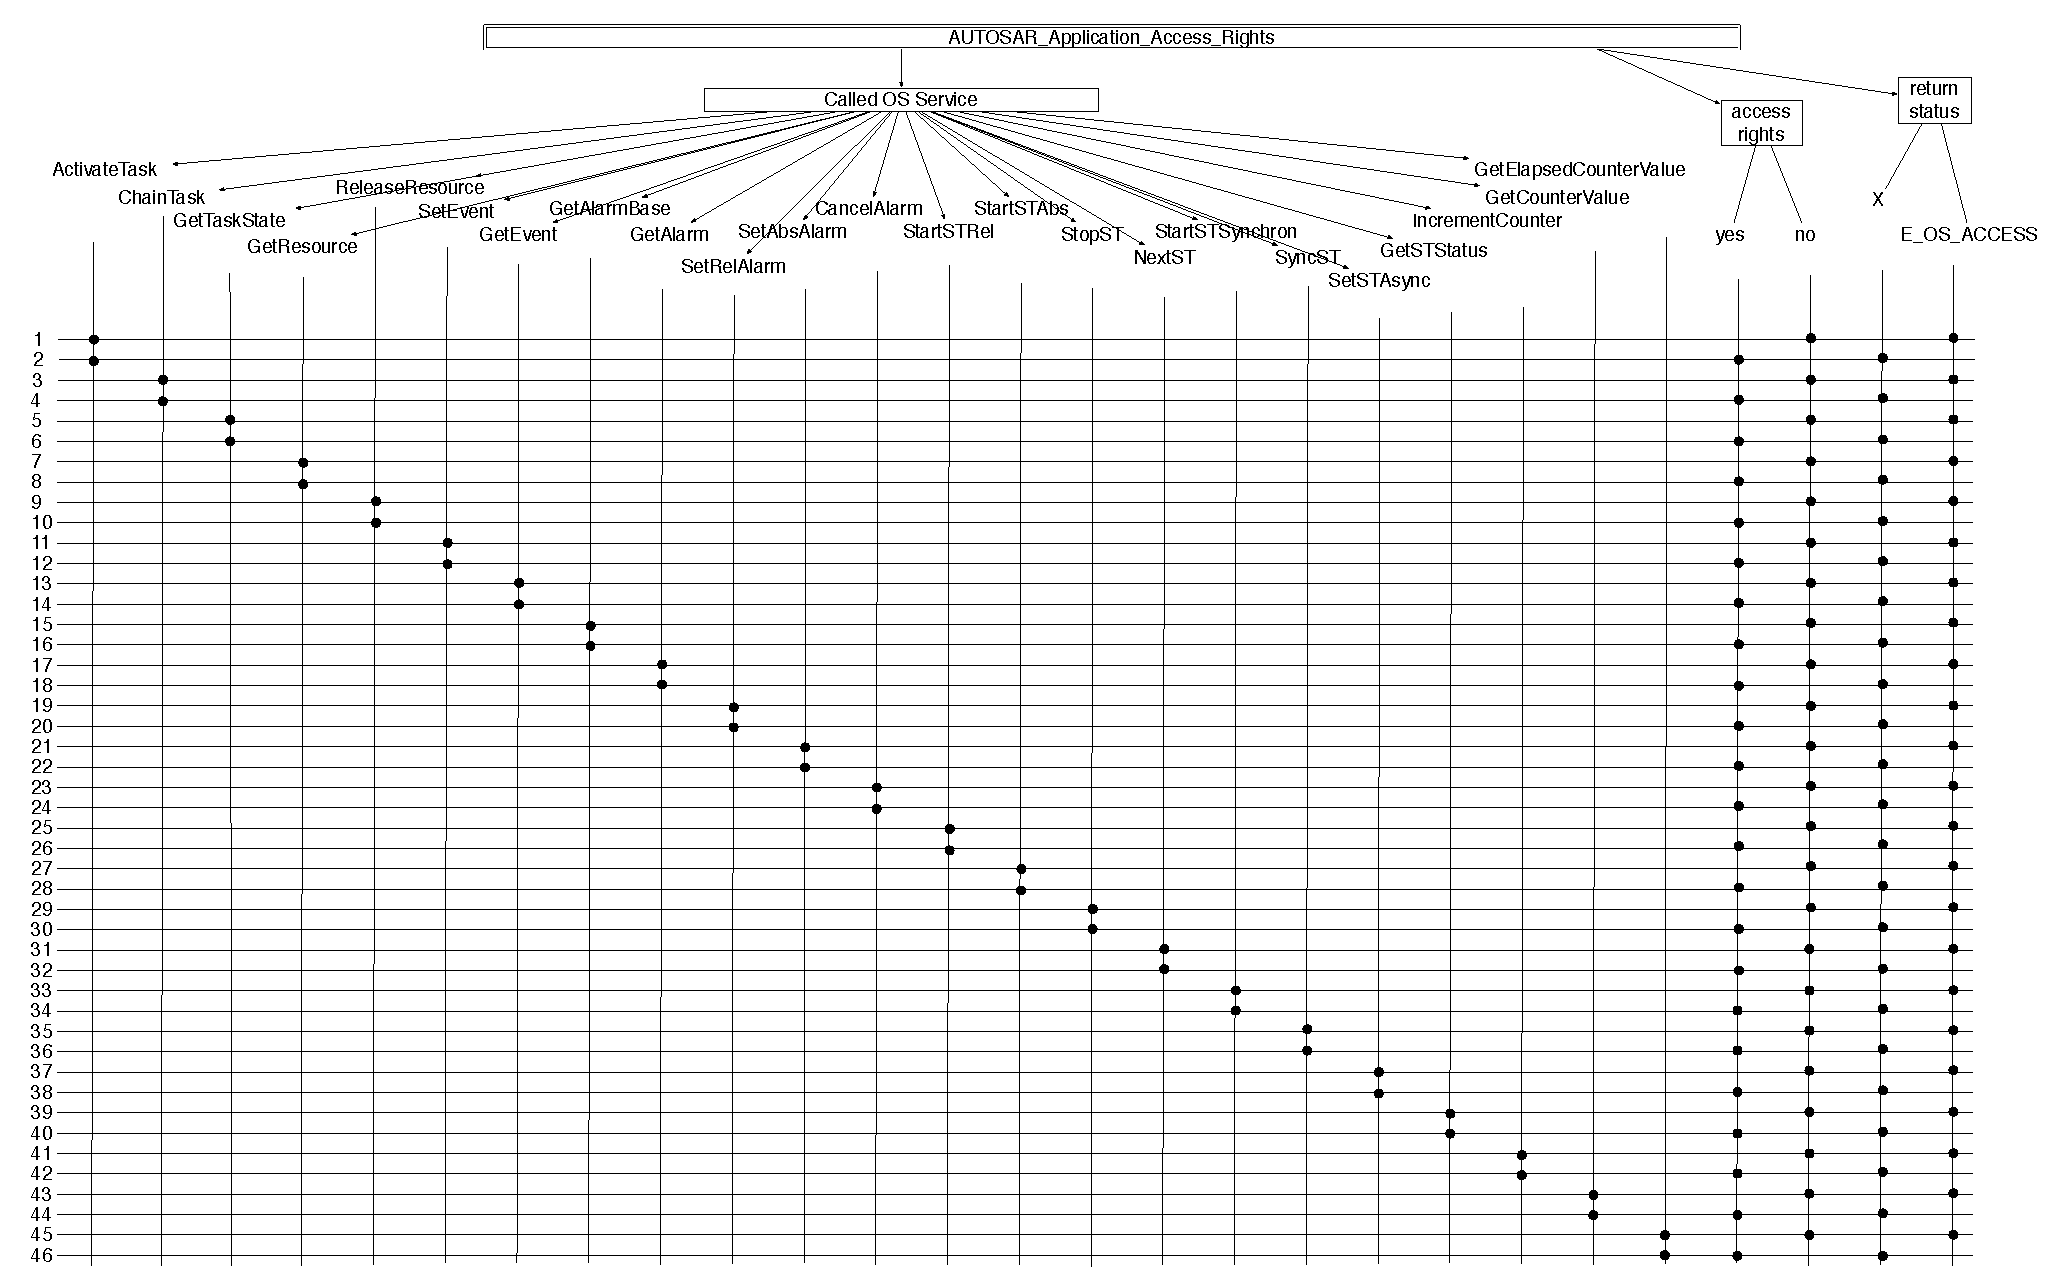
\includegraphics[width=1\textheight, angle=90]{graphics/AUTOSAR_Application_Access_Rights.pdf}
	\end{figure}

	\begin{supertabular}{|p{\Li}|p{\Lii}|p{\Liii}|p{\Liiii}|} \hline
	1	& Call ActivateTask() for a task which can be accessed by the \textit{running} task/ISR2 				& Service returns E\_OK if no error		& OS448 \\ \hline
	2	& Call ActivateTask() for a task which can't be accessed by the \textit{running} task/ISR2 				& Service returns E\_OS\_ACCESS		& OS056, OS448  \\ \hline
	3	& Call ChainTask() for a task which can be accessed by the \textit{running} task/ISR2 				& Service returns E\_OK if no error		& \\ \hline
	4	& Call ChainTask() for a task which can't be accessed by the \textit{running} task/ISR2 				& Service returns E\_OS\_ACCESS		& \\ \hline
	5	& Call GetTaskState() for a task which can be accessed by the \textit{running} task/ISR2 				& Service returns E\_OK if no error		& \\ \hline
	6	& Call GetTaskState() for a task which can't be accessed by the \textit{running} task/ISR2				& Service returns E\_OS\_ACCESS		& \\ \hline
	7	& Call GetResource() for a task which can be accessed by the \textit{running} task/ISR2 				& Service returns E\_OK if no error		& \\ \hline
	8	& Call GetResource() for a task which can't be accessed by the \textit{running} task/ISR2				& Service returns E\_OS\_ACCESS		& \\ \hline
	9	& Call ReleaseResource() for a task which can be accessed by the \textit{running} task/ISR2 			& Service returns E\_OK if no error		& \\ \hline
	10	& Call ReleaseResource() for a task which can't be accessed by the \textit{running} task/ISR2			& Service returns E\_OS\_ACCESS		& \\ \hline
	11	& Call SetEvent() for a task which can be accessed by the \textit{running} task/ISR2 				& Service returns E\_OK if no error		& \\ \hline
	12	& Call SetEvent() for a task which can't be accessed by the \textit{running} task/ISR2				& Service returns E\_OS\_ACCESS		& \\ \hline
	13	& Call GetEvent() for a task which can be accessed by the \textit{running} task/ISR2 				& Service returns E\_OK if no error		& \\ \hline
	14	& Call GetEvent() for a task which can't be accessed by the \textit{running} task/ISR2				& Service returns E\_OS\_ACCESS		& \\ \hline
	15	& Call GetAlarmBase() for a task which can be accessed by the \textit{running} task/ISR2		 	& Service returns E\_OK if no error		& \\ \hline
	16	& Call GetAlarmBase() for a task which can't be accessed by the \textit{running} task/ISR	2			& Service returns E\_OS\_ACCESS		& \\ \hline
	17	& Call GetAlarm() for a task which can be accessed by the \textit{running} task/ISR2 				& Service returns E\_OK if no error		& \\ \hline
	18	& Call GetAlarm() for a task which can't be accessed by the \textit{running} task/ISR2				& Service returns E\_OS\_ACCESS		& \\ \hline
	19	& Call SetRelAlarm() for a task which can be accessed by the \textit{running} task/ISR2 				& Service returns E\_OK if no error		& \\ \hline
	20	& Call SetRelAlarm() for a task which can't be accessed by the \textit{running} task/ISR2				& Service returns E\_OS\_ACCESS		& \\ \hline
	21	& Call SetAbsAlarm() for a task which can be accessed by the \textit{running} task/ISR2 				& Service returns E\_OK if no error		& \\ \hline
	22	& Call SetAbsAlarm() for a task which can't be accessed by the \textit{running} task/ISR2				& Service returns E\_OS\_ACCESS		& \\ \hline
	23	& Call CancelAlarm() for a task which can be accessed by the \textit{running} task/ISR2 				& Service returns E\_OK if no error		& \\ \hline
	24	& Call CancelAlarm() for a task which can't be accessed by the \textit{running} task/ISR2				& Service returns E\_OS\_ACCESS		& \\ \hline
	25	& Call StartScheduleTableRel() for a task which can be accessed by the \textit{running} task/ISR2 		& Service returns E\_OK if no error		& \\ \hline
	26	& Call StartScheduleTableRel() for a task which can't be accessed by the \textit{running} task/ISR2		& Service returns E\_OS\_ACCESS		& \\ \hline
	27	& Call StartScheduleTableAbs() for a task which can be accessed by the \textit{running} task/ISR2 		& Service returns E\_OK if no error		& \\ \hline
	28	& Call StartScheduleTableAbs() for a task which can't be accessed by the \textit{running} task/ISR2		& Service returns E\_OS\_ACCESS		& \\ \hline
	29	& Call StopScheduleTable() for a task which can be accessed by the \textit{running} task/ISR2 		& Service returns E\_OK if no error		& \\ \hline
	30	& Call StopScheduleTable() for a task which can't be accessed by the \textit{running} task/ISR2		& Service returns E\_OS\_ACCESS		& \\ \hline
	31	& Call NextScheduleTable() for a task which can be accessed by the \textit{running} task/ISR2 		& Service returns E\_OK if no error		& \\ \hline
	32	& Call NextScheduleTable() for a task which can't be accessed by the \textit{running} task/ISR2		& Service returns E\_OS\_ACCESS		& \\ \hline
	33	& Call StartScheduleTableSynchron() for a task which can be accessed by the \textit{running} task/ISR2 	& Service returns E\_OK if no error		& \\ \hline
	34	& Call StartScheduleTableSynchron() for a task which can't be accessed by the \textit{running} task/ISR2	& Service returns E\_OS\_ACCESS		& \\ \hline
	35	& Call SyncScheduleTable() for a task which can be accessed by the \textit{running} task/ISR2 		& Service returns E\_OK if no error		& \\ \hline
	36	& Call SyncScheduleTable() for a task which can't be accessed by the \textit{running} task/ISR2		& Service returns E\_OS\_ACCESS		& \\ \hline
	37	& Call SetScheduleTableAsync() for a task which can be accessed by the \textit{running} task/ISR2 	& Service returns E\_OK if no error		& \\ \hline
	38	& Call SetScheduleTableAsync() for a task which can't be accessed by the \textit{running} task/ISR2	& Service returns E\_OS\_ACCESS		& \\ \hline
	39	& Call GetScheduleTableStatus() for a task which can be accessed by the \textit{running} task/ISR2 	& Service returns E\_OK if no error		& \\ \hline
	40	& Call GetScheduleTableStatus() for a task which can't be accessed by the \textit{running} task/ISR2	& Service returns E\_OS\_ACCESS		& \\ \hline
	41	& Call IncrementCounter() for a task which can be accessed by the \textit{running} task/ISR2 			& Service returns E\_OK if no error		& \\ \hline
	42	& Call IncrementCounter() for a task which can't be accessed by the \textit{running} task/ISR2			& Service returns E\_OS\_ACCESS		& \\ \hline
	43	& Call GetCounterValue() for a task which can be accessed by the \textit{running} task/ISR2 			& Service returns E\_OK if no error		& \\ \hline
	44	& Call GetCounterValue() for a task which can't be accessed by the \textit{running} task/ISR2			& Service returns E\_OS\_ACCESS		& \\ \hline
	45	& Call GetElapsedCounterValue() for a task which can be accessed by the \textit{running} task/ISR2	& Service returns E\_OK if no error		& \\ \hline
	46	& Call GetElapsedCounterValue() for a task which can't be accessed by the \textit{running} task/ISR2	& Service returns E\_OS\_ACCESS		& \\ \hline	
	\end{supertabular}

	\subsubsection{Access Rights for objects from OIL file}
	OS Requirements: 056
	
	\begin{figure}[htbp] %  figure placement: here, top, bottom, or page
  		\centering
		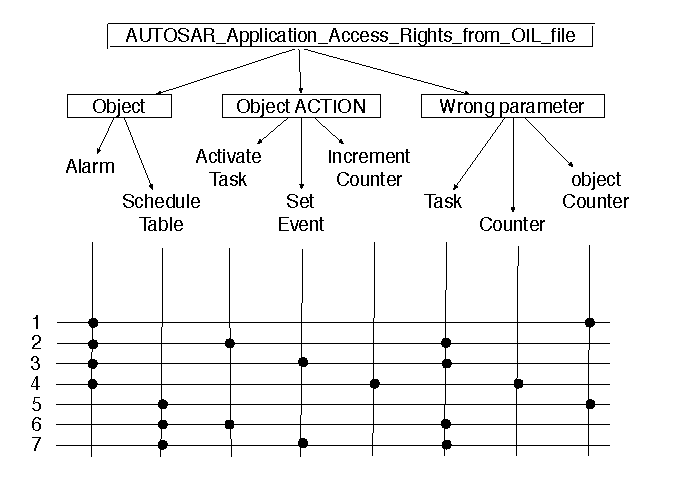
\includegraphics[width=0.5\textwidth]{graphics/AUTOSAR_Application_Access_Rights_OIL.pdf}
	\end{figure}

	\begin{supertabular}{|p{\Li}|p{\Lii}|p{\Liii}|p{\Liiii}|} \hline
	1	& Alarm's Counter doesn't belong to the same application of the alarm and the alarm has no access rights to the counter's application								& error : Counter C doesn't belong to the same application of alarm A		& \\ \hline		
	2	& Action of an alarm results in a ActivateTask. Action's Task doesn't belong to the same application of the alarm and the alarm has no access rights to the task's application	& error : Task T doesn't belong to the same application of alarm A		& \\ \hline
	3	& Action of an alarm results in a SetEvent. Action's Task doesn't belong to the same application of the alarm and the alarm has no access rights to the task's application	& error : Task T doesn't belong to the same application of alarm A		& \\ \hline
	4	& Action of an alarm results in a IncrementCounter. Action's Counter doesn't belong to the same application of the alarm and the alarm has no access rights to the counter's application	& error : Counter C doesn't belong to the same application of alarm A	& \\ \hline
	5	& Schedule table's Counter doesn't belong to the same application of the schedule table and the schedule table has no access rights to the counter's application						& error : Counter C doesn't belong to the same application of schedule table S		& \\ \hline		
	6	& Action of an expiry point of a schedule table results in a ActivateTask. Action's Task doesn't belong to the same application of the schedule table and the schedule table has no access rights to the task's application	& error : Task T doesn't belong to the same application of schedule table S		& \\ \hline
	7	& Action of an expiry point of a schedule table results in a SetEvent. Action's Task doesn't belong to the same application of the schedule table and the schedule table has no access rights to the task's application		& error : Task T doesn't belong to the same application of schedule table S		& \\ \hline
	\end{supertabular}
	
	
	
	
	% AUTOSAR - SERVICE PROTECTION %
	\subsection{AUTOSAR - Service Protection}
	OS Requirements : 52, 69, 70, 71, 92, 93, 239, 368, 369\\
	Test case 11 can't be tested because enabling/resuming API service call doesn't return.\\	
	As specified in AUTOSAR OS Specifications, when an API service call happens when interrupts are disabled, the service should be ignored and should return E\_OS\_DISABLEDINT when the service return a StatusType (OS093, Test Case 10). The ErrorHook(s) is(are) called.\\
	As nothing is described for API services which doesn't return a StatusType, we decide executing the service correctly, calling the Errorhook(s) with E\_OS\_DISABLEDINT as sequence 5 in the procedure (See GetActiveApplicationMode(), GetApplicationID(), GetISRID(), CheckObjectAccess(), CheckObjectOwnership()). \\
	
	\begin{figure}[htbp] %  figure placement: here, top, bottom, or page
  		\centering
		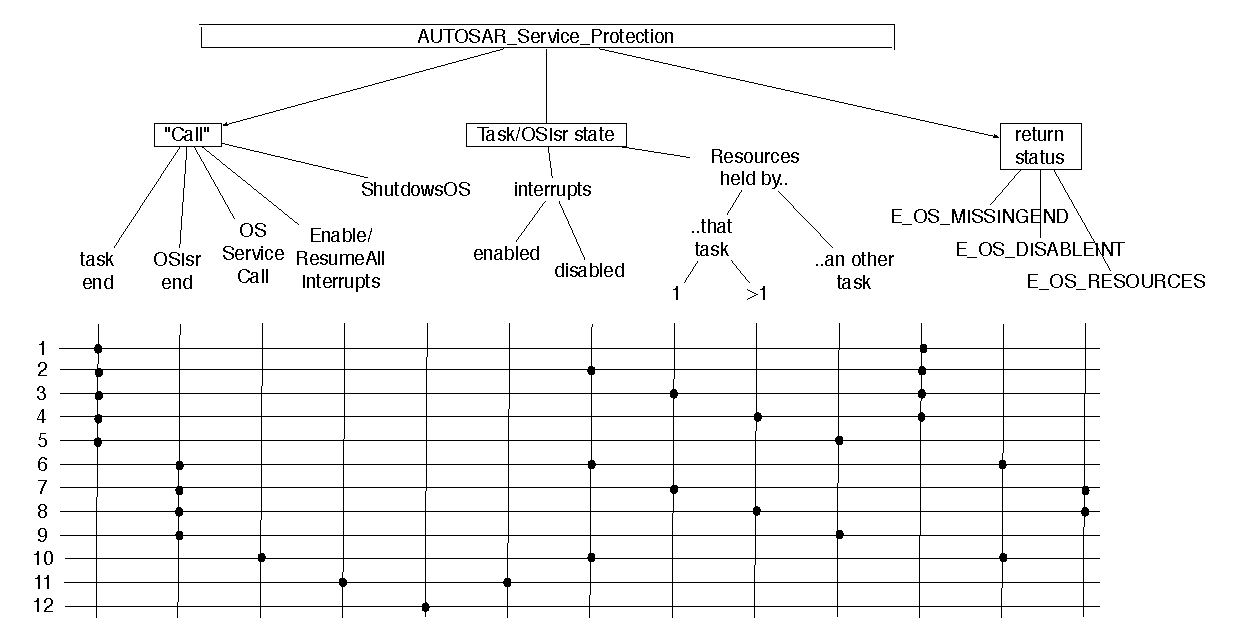
\includegraphics[width=0.8\textwidth]{graphics/AUTOSAR_Service_Protection.pdf}
	\end{figure}

	\begin{supertabular}{|p{\Li}|p{\Lii}|p{\Liii}|p{\Liiii}|} \hline
	1	& Ending a task without making a TerminateTask() or ChainTask() call		& The OS shall terminate the task, call the errorhook (if configured) with status E\_OS\_MISSINGEND before leaving RUNNING state and call the posttaskhook (is configured)			& OS052, OS069 \\ \hline
	2	& Ending a task without making a TerminateTask() with interrupts disabled	& The OS shall terminate the task, call the errorhook (if configured) with status E\_OS\_MISSINGEND and enabling interrupts				& OS239 \\ \hline
	3	& Ending a task without making a TerminateTask(), holding 1 resource		& The OS shall terminate the task, call the errorhook (if configured) with status E\_OS\_MISSINGEND and release the resource				& OS070 \\ \hline
	4	& Ending a task without making a TerminateTask(), holding several resources		& The OS shall terminate the task, call the errorhook (if configured) with status E\_OS\_MISSINGEND and release resources				& OS070 \\ \hline
	5	& Ending a task without making a TerminateTask(), an other task holding resource(s)	& The OS shall terminate the task, call the errorhook (if configured) with status E\_OS\_MISSINGEND 								& OS070 \\ \hline
	6	& Ending an ISR2 with interrupts disabled							& The OS shall call the errorhook (if configured) with status E\_OS\_DISABLEDINT and enabling interrupts			& OS368 \\ \hline
	7	& Ending an ISR2, holding 1 resource						 		& The OS shall call the errorhook (if configured) with status E\_OS\_RESOURCE and release the resource			& OS369 \\ \hline
	8	& Ending an ISR2, holding several resources							& The OS shall call the errorhook (if configured) with status E\_OS\_RESOURCE and release resources		& OS369 \\ \hline
	9	& Ending an ISR2, an other task holding resource(s)					& The OS shall call the errorhook (if configured) with status E\_OS\_RESOURCE 			& OS369 \\ \hline
	10	& Call an OS service when interrupts are disabled						& Service (which can) returns E\_OS\_DISABLEDINT, ignoring the service & OS093 \\  \hline
	11	& Enabling/Resuming ingterrupts when interrupts are already enabled 		& Service ignored		& OS092 \\ \hline
	12	& Call ShutdownOS()											& PostTaskHook is not performed (even if PostTaskHook is configured) 		& OS071 \\ \hline
	\end{supertabular}
		
		
	% AUTOSAR - MEMORY PROTECTION %
	\subsection{AUTOSAR - Memory Protection} \label{memprot}
	OS Requirements : 26, 27, 44, 81, 83, 86, 87, 195, 196, 198, 207, 208, 209, 355, 356.\\
	Test case 14, 15, 16, 18 (the own peripheral part) are not tested yet.\\
	
	\begin{figure}[htbp] %  figure placement: here, top, bottom, or page
  		\centering
		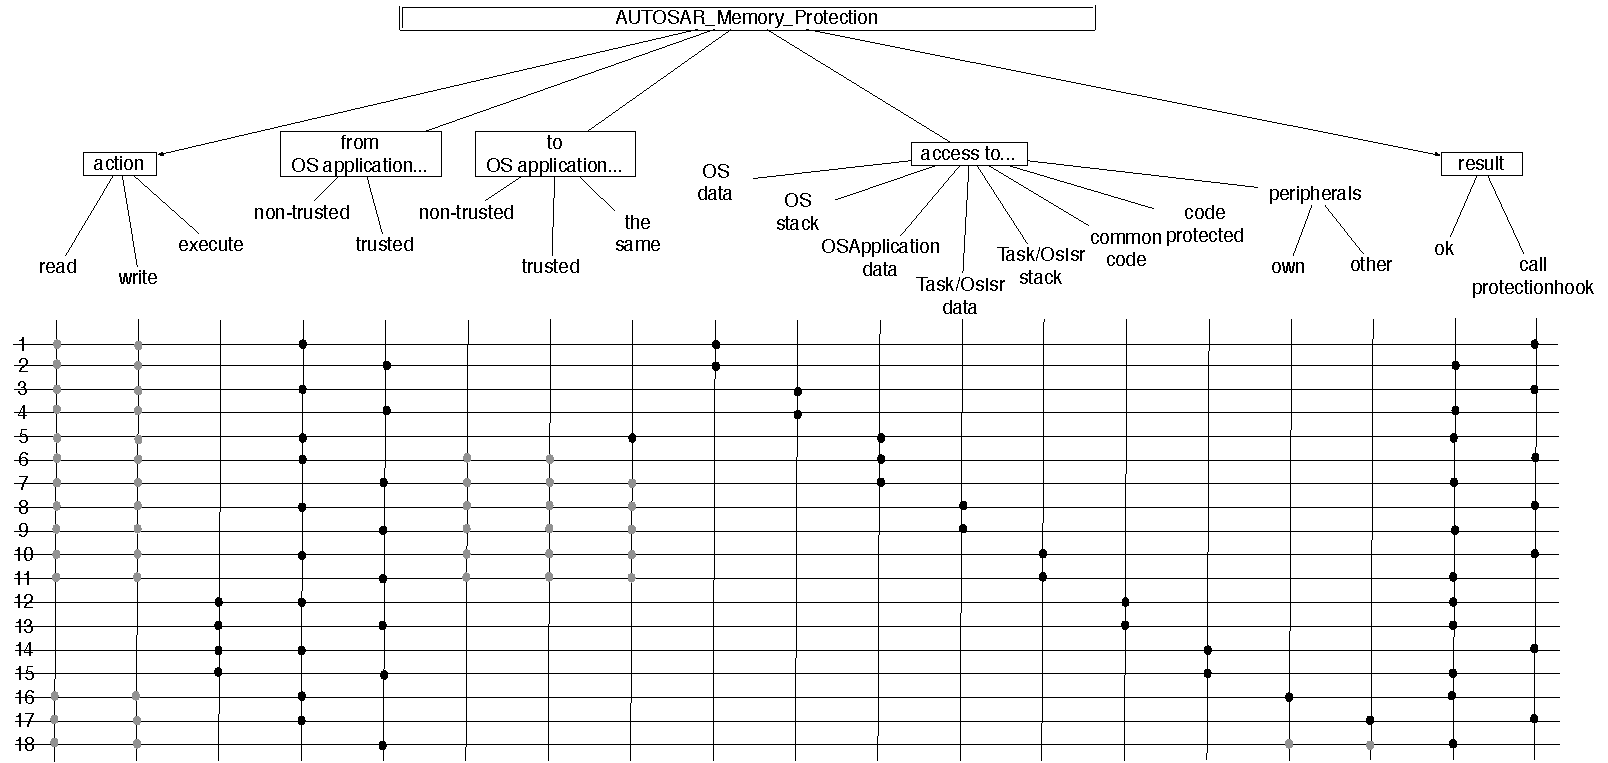
\includegraphics[width=1\textwidth]{graphics/AUTOSAR_Memory_Protection.pdf}
	\end{figure}
	
	As you can see above, the test case 1 correspond to two test cases : a Read test case (1a) and a Write test case (1b). Moreover, the test case 7 (and some others) correspond to six test cases as described in the table below.\\
	
	\begin{figure}[htbp] %  figure placement: here, top, bottom, or page
  		\centering
		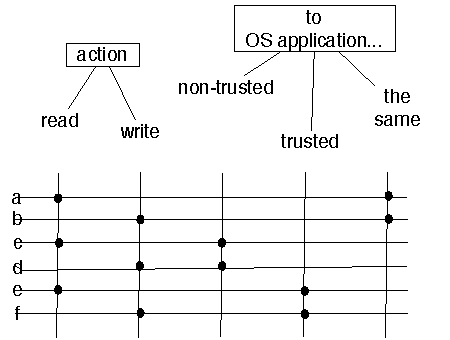
\includegraphics[width=0.3\textwidth]{graphics/AUTOSAR_Memory_Protection_test_cases.pdf}
	\end{figure}
	
	
	\begin{supertabular}{|p{\Li}|p{\Lii}|p{\Liii}|p{\Liiii}|} \hline
	1a	& Read OS datas from non-trusted OS application 		& The OS shall call the protectionhook (if configured) with status E\_OS\_PROTECTION\_MEMORY			& OS198 \\ \hline
	1b	& Write OS datas from non-trusted OS application 		& The OS shall call the protectionhook (if configured) with status E\_OS\_PROTECTION\_MEMORY			& OS198 \\ \hline
	2a	& Read OS datas from trusted OS application 			& Access allowed																		& OS198 \\ \hline
	2b	& Write OS datas from trusted OS application 			& Access allowed																		& OS198 \\ \hline
	3a	& Read OS stack from non-trusted OS application 		& The OS shall call the protectionhook (if configured) with status E\_OS\_PROTECTION\_MEMORY			& OS198 \\ \hline
	3b	& Write OS stack from non-trusted OS application 		& The OS shall call the protectionhook (if configured) with status E\_OS\_PROTECTION\_MEMORY			& OS198 \\ \hline
	4a	& Read OS stack from trusted OS application 			& Access allowed																		& OS198 \\ \hline
	4b	& Write OS stack from trusted OS application 			& Access allowed																		& OS198 \\ \hline
	5a	& Read its own OS application's datas from non-trusted OS application	&  Access allowed															& OS086 \\ \hline
	5b	& Write its own OS application's datas from non-trusted OS application	&  Access allowed															& OS086 \\ \hline
	
	6c	& Read non-trusted OS application's datas from non-trusted OS application	&  The OS shall call the protectionhook (if configured) with status E\_OS\_PROTECTION\_MEMORY	& OS026 \\ \hline
	6d	& Write non-trusted OS application's datas from non-trusted OS application	&  The OS shall call the protectionhook (if configured) with status E\_OS\_PROTECTION\_MEMORY	& OS207 \\ \hline
	6e	& Read trusted other OS application's datas from non-trusted OS application	&  The OS shall call the protectionhook (if configured) with status E\_OS\_PROTECTION\_MEMORY	& OS026 \\ \hline
	6f	& Write trusted other OS application's datas from non-trusted OS application	&  The OS shall call the protectionhook (if configured) with status E\_OS\_PROTECTION\_MEMORY	& OS207 \\ \hline
	
	7a	& Read its own OS application's datas from trusted OS application			&  Access allowed															& According to OS026  \\ \hline
	7b	& Write its own OS application's datas from trusted OS application			&  Access allowed															& OS086  \\ \hline
	7c	& Read non-trusted OS application's datas from trusted OS application		&  Access allowed															& According to OS026 \\ \hline
	7d	& Write non-trusted OS application's datas from trusted OS application		&  Access allowed															& According to OS207 \\ \hline
	7e	& Read trusted OS application's datas from trusted OS application			&  Access allowed															& According to OS026  \\ \hline
	7f	& Write trusted OS application's datas from trusted OS application			&  Access allowed															& According to OS207  \\ \hline
	
	8a	& Read Task/OsIsr's datas of the same non-trusted OS application			& The OS shall call the protectionhook (if configured) with status E\_OS\_PROTECTION\_MEMORY	& OS195 \\ \hline
	8b	& Write Task/OsIsr's datas of the same non-trusted OS application			& The OS shall call the protectionhook (if configured) with status E\_OS\_PROTECTION\_MEMORY	& OS195 \\ \hline
	8c	& Read Task/OsIsr's datas of an other non-trusted OS application from non-trusted OS application 		& The OS shall call the protectionhook (if configured) with status E\_OS\_PROTECTION\_MEMORY	& OS356 \\ \hline
	8d	& Read Task/OsIsr's datas of an other non-trusted OS application from non-trusted OS application 		& The OS shall call the protectionhook (if configured) with status E\_OS\_PROTECTION\_MEMORY	& OS356 \\ \hline
	8e	& Read Task/OsIsr's datas of a trusted OS application from non-trusted OS application 				& The OS shall call the protectionhook (if configured) with status E\_OS\_PROTECTION\_MEMORY	& OS356 \\ \hline
	8f	& Write Task/OsIsr's datas of a trusted OS application from non-trusted OS application 				& The OS shall call the protectionhook (if configured) with status E\_OS\_PROTECTION\_MEMORY	& OS356 \\ \hline
	
	9a	& Read Task/OsIsr's datas of the same trusted OS application 				& Access allowed 									& OS087 \\ \hline
	9b	& Write Task/OsIsr's datas of the same trusted OS application 				& Access allowed 									& OS087 \\ \hline
	9c	& Read Task/OsIsr's datas of a non-trusted OS application from trusted OS application		& Access allowed 									& OS087 \\ \hline
	9d	& Write Task/OsIsr's datas of a non-trusted OS application from trusted OS application		& Access allowed 									& OS087 \\ \hline
	9e	& Read Task/OsIsr's datas of an other trusted OS application from trusted OS application		& Access allowed 									& OS087 \\ \hline
	9f	& Write Task/OsIsr's datas of an other trusted OS application from trusted OS application		& Access allowed 									& OS087 \\ \hline
		
	10a	& Read Task/OsIsr's stack of the same non-trusted OS application 			& The OS shall call the protectionhook (if configured) with status E\_OS\_PROTECTION\_MEMORY	& OS208 \\ \hline
	10b	& Write Task/OsIsr's stack of the same non-trusted OS application 			& The OS shall call the protectionhook (if configured) with status E\_OS\_PROTECTION\_MEMORY	& OS208 \\ \hline
	10c	& Read Task/OsIsr's stack of an other non-trusted OS application from non-trusted OS application		& The OS shall call the protectionhook (if configured) with status E\_OS\_PROTECTION\_MEMORY	& OS355 \\ \hline
	10d	& Write Task/OsIsr's stack of an other non-trusted OS application from non-trusted OS application		& The OS shall call the protectionhook (if configured) with status E\_OS\_PROTECTION\_MEMORY	& OS355 \\ \hline
	10e	& Read Task/OsIsr's stack of a trusted OS application from non-trusted OS application				& The OS shall call the protectionhook (if configured) with status E\_OS\_PROTECTION\_MEMORY	& OS355 \\ \hline
	10f	& Write Task/OsIsr's stack of a trusted OS application from non-trusted OS application				& The OS shall call the protectionhook (if configured) with status E\_OS\_PROTECTION\_MEMORY	& OS355 \\ \hline
	
	11a	& Read Task/OsIsr's stack of the same trusted OS application 				& Access allowed 									& OS196 \\ \hline
	11b	& Write Task/OsIsr's stack of the same trusted OS application 				& Access allowed 									& OS196 \\ \hline
	11c	& Read Task/OsIsr's stack of a non-trusted OS application from trusted OS application		& Access allowed 									& OS196 \\ \hline
	11d	& Write Task/OsIsr's stack of a non-trusted OS application from trusted OS application		& Access allowed 									& OS196 \\ \hline
	11e	& Read Task/OsIsr's stack of an other trusted OS application from trusted OS application		& Access allowed 									& OS196 \\ \hline
	11f	& Write Task/OsIsr's stack of an other trusted OS application from trusted OS application		& Access allowed 									& OS196 \\ \hline

	12	& Execute sharde library code from non-trusted OS application 		 	& Access allowed 															& OS081 \\ \hline
	13	& Execute sharde library code from trusted OS application 			 	& Access allowed 															& OS081 \\ \hline
	14	& Execute protected (an OS application can protect its code section) code from non-trusted OS application 	& The OS shall call the protectionhook (if configured) with status E\_OS\_PROTECTION\_MEMORY	& OS027 \\ \hline
	15	& Execute protected (an OS application can protect its code section) code from trusted OS application 		& Access allowed									& OS027 \\ \hline
	
	16a 	& Read its own peripherals from non-trusted OS application				& Access allowed															& OS083 \\ \hline
	16b 	& Write to its own peripherals from non-trusted OS application				& Access allowed															& OS083 \\ \hline
	17c 	& Read other peripherals from non-trusted OS application			& The OS shall call the protectionhook (if configured) with status E\_OS\_PROTECTION\_MEMORY	& according to OS083 \\ \hline
	17d 	& Write to other peripherals from non-trusted OS application			& The OS shall call the protectionhook (if configured) with status E\_OS\_PROTECTION\_MEMORY	& according to OS083 \\ \hline
	18a 	& Read its own peripherals from trusted OS application					& Access allowed															& OS209 \\ \hline
	18b 	& Write its own peripherals from trusted OS application					& Access allowed															& OS209 \\ \hline
	18c 	& Read other peripherals from trusted OS application					& Access allowed															& OS209 \\ \hline
	18d 	& Write other peripherals from trusted OS application					& Access allowed															& OS209 \\ \hline
	\end{supertabular}
	
	% AUTOSAR - TIMING PROTECTION %
	\subsection{AUTOSAR - Timing Protection}
	OS Requirements : (28), (89), (397)\\
	
	\subsubsection{Execution Time Budget}
	OS Requirements : 64, 210, 473, 474\\
	
	\begin{figure}[htbp] %  figure placement: here, top, bottom, or page
  		\centering
		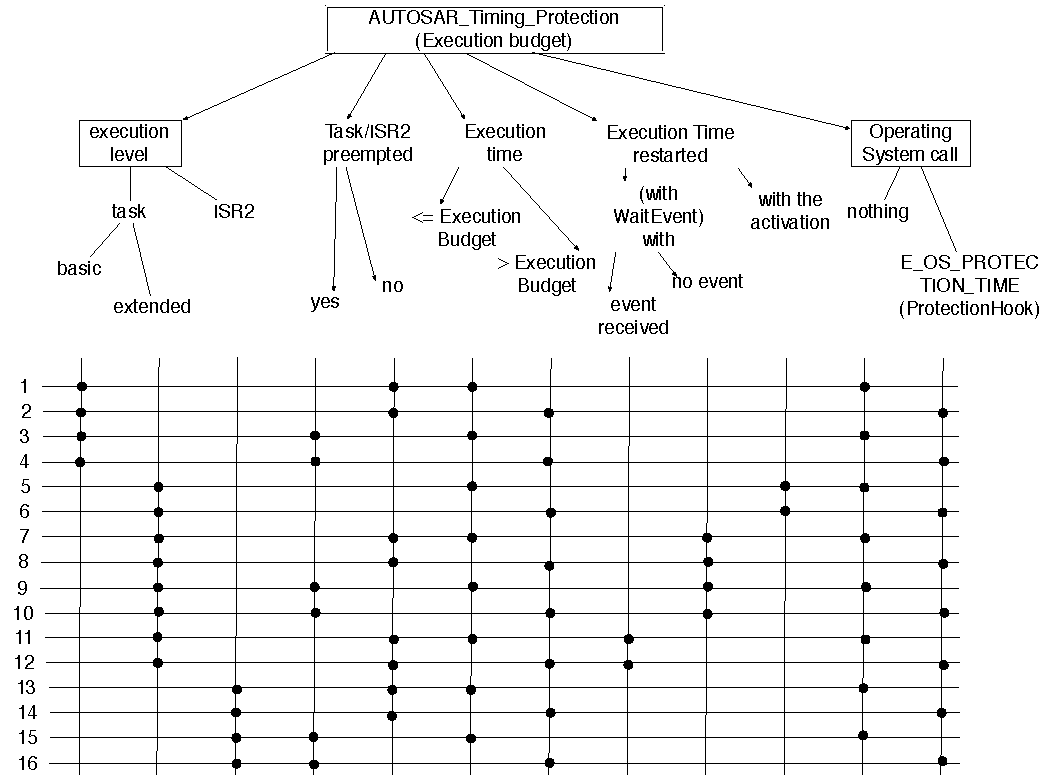
\includegraphics[width=1\textwidth]{graphics/AUTOSAR_Timing_Protection_Execution_Budget.pdf}
	\end{figure}
	
	\begin{supertabular}{|p{\Li}|p{\Lii}|p{\Liii}|p{\Liiii}|} \hline
	1	& Execution Time of a non-preempted basic task is less than the Execution Budget	& 						& OS473 \\ \hline
	2	& Execution Time of a non-preempted basic task reaches the Execution Budget	&  The OS shall call the protectionhook (if configured) with status E\_OS\_PROTECTION\_TIME	& OS064  \\ \hline
	3	& Execution Time of a preempted basic task is less than the Execution Budget		& 						&  \\ \hline
	4	& Execution Time of a preempted basic task reaches the Execution Budget		&  The OS shall call the protectionhook (if configured) with status E\_OS\_PROTECTION\_TIME	& OS064 \\ \hline
	5	& Execution Time of an extended task which has been reset by the activation of the task until WaitEvent API calls	& 			&  \\ \hline
	6	& Execution Time of an extended task which has been reset by the activation of the task but never comes to the WaitEvent API	& The OS shall call the protectionhook (if configured) with status E\_OS\_PROTECTION\_TIME		& OS064 \\ \hline
	7	& Execution Time (restarted by WaitEvent without event set) of a non-preempted extended task is less than the Execution Budget	& 									& OS473 \\ \hline
	8	& Execution Time (restarted by WaitEvent without event set) of a non-preempted extended task reaches the Execution Budget	&  The OS shall call the protectionhook (if configured) with status E\_OS\_PROTECTION\_TIME		& OS064 \\ \hline
	9	& Execution Time (restarted by WaitEvent without event set) of a preempted basic task is less than the Execution Budget		& 									& OS473  \\ \hline
	10	& Execution Time (restarted by WaitEvent without event set) of a preempted basic task reaches the Execution Budget			&  The OS shall call the protectionhook (if configured) with status E\_OS\_PROTECTION\_TIME		& OS064 \\ \hline
	11	& Execution Time (restarted by WaitEvent with the event(s) set) of a non-preempted extended task is less than the Execution Budget	& 								&  \\ \hline
	12	& Execution Time (restarted by WaitEvent with the event(s) set) of a non-preempted extended task reaches the Execution Budget	&  The OS shall call the protectionhook (if configured) with status E\_OS\_PROTECTION\_TIME		& OS064 \\ \hline
	13	& Execution Time of a preempted ISR2 is less than the Execution Budget	& 						& OS474 \\ \hline
	14	& Execution Time of a preempted ISR2 reaches the Execution Budget		&  The OS shall call the protectionhook (if configured) with status E\_OS\_PROTECTION\_TIME 	& OS210 \\ \hline
	15	& Execution Time of a preempted ISR2 is less than the Execution Budget	& 						&  \\ \hline
	16	& Execution Time of a preempted ISR2 reaches the Execution Budget		&  The OS shall call the protectionhook (if configured) with status E\_OS\_PROTECTION\_TIME	& OS210 \\ \hline
	\end{supertabular}
	
	\subsubsection{Time Frame}
	OS Requirements : 48, (465), 466, 467, 469, (470), 471, 472\\

	\begin{figure}[htbp] %  figure placement: here, top, bottom, or page
  		\centering
		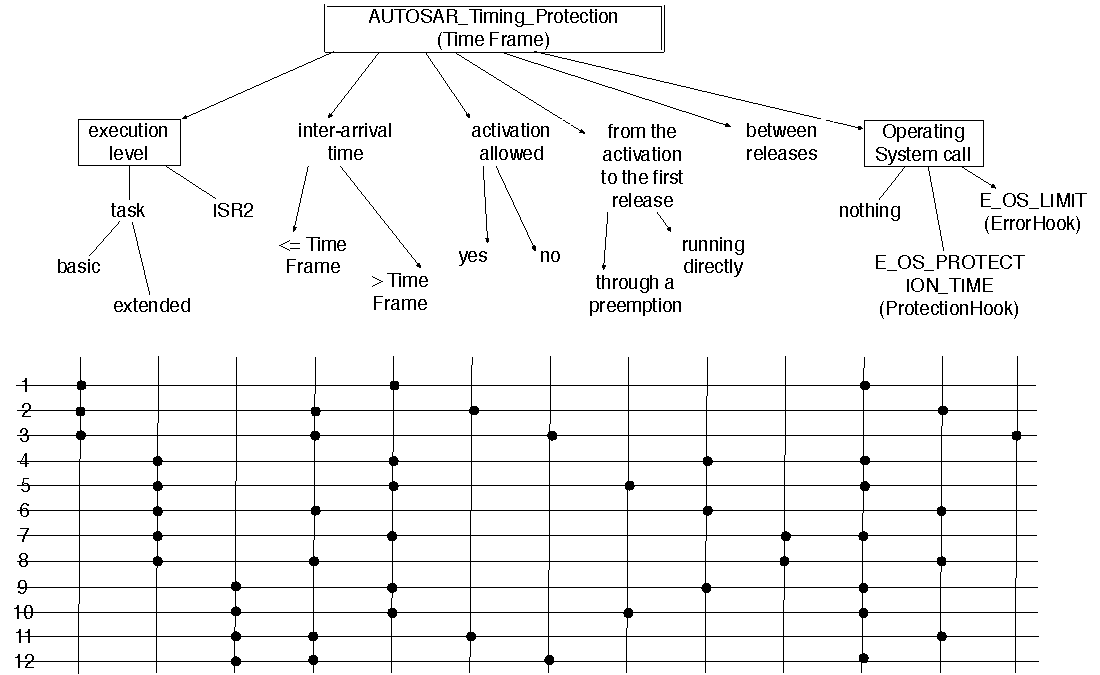
\includegraphics[width=1\textwidth]{graphics/AUTOSAR_Timing_Protection_Time_Frame.pdf}
	\end{figure}
	
	\begin{supertabular}{|p{\Li}|p{\Lii}|p{\Liii}|p{\Liiii}|} \hline
	1	& Basic task inter-arrival time is greater than Time Frame								& 													&  \\ \hline
	2	& Basic task inter-arrival time is lower than Time Frame (and the task activation is allowed)	&  The OS shall call the protectionhook (if configured) with status E\_OS\_PROTECTION\_ARRIVAL 	& OS466 \\ \hline
	3	& Basic task inter-arrival time is lower than Time Frame (and the task activation is not allowed)	&  The OS shall call the errorhook (if configured) with status E\_OS\_LIMIT 				& OS469 \\ \hline
	4	& Extended task inter-arrival time is greater than Time Frame. Time from the activation to the first release (task running directly)	& 						& \\ \hline
	5	& Extended task inter-arrival time is greater than Time Frame. Time from the activation to the first release (task running after a preemption to test the inter-arrival time is well started at the activation and not from the running point)	& & \\ \hline
	6	& Extended task inter-arrival time is lower than Time Frame. Time from the activation to the first release (task running directly) & The OS shall call the protectionhook (if configured) with status E\_OS\_PROTECTION\_ARRIVAL & OS467 \\ \hline
	7	& Extended task inter-arrival time is greater than Time Frame. Time between two releases.	&													 & OS472 \\ \hline
	8	& Extended task inter-arrival time is lower than Time Frame. Time between two releases.	& The OS shall call the protectionhook (if configured) with status E\_OS\_PROTECTION\_ARRIVAL 	& OS467 \\ \hline
	9	& ISR2 inter-arrival time is greater than Time Frame	(ISR2 running directly)				& 													&  \\ \hline
	10	& ISR2 inter-arrival time is greater than Time Frame (ISR2 running after a preemption to test the inter-arrival time is well started at the activation and not from the running point)	&  				& OS471 \\ \hline
	11	& ISR2 inter-arrival time is lower than Time Frame (the ISR2 is not running)				& The OS shall call the protectionhook (if configured) with status E\_OS\_PROTECTION\_ARRIVAL 	& OS048 \\ \hline
	12	& Basic task inter-arrival time is lower than Time Frame (the ISR2 is running)				& 													&  \\ \hline
	\end{supertabular}
	
	\subsubsection{Resource Locking and Interrupt Disabling}
	OS Requirements : (33), (37)\\

	
	% AUTOSAR - TRUSTED FUNCTION %
	%\subsection{AUTOSAR - Trusted function}
	
	% AUTOSAR - PROTECTION ERROR HANDLING %
	%\subsection{AUTOSAR - Protection error handling}
	
	% AUTOSAR - HOOK FUNCTIONS %
	%\subsection{AUTOSAR - Hook functions}
	
	% AUTOSAR - SYSTEM SCALABILITY %
	%\subsection{AUTOSAR - System scalability}
	
	
	
\appendix
\section{Interrupts Management} \label{interrupts_management}
	\begin{figure}[htbp] %  figure placement: here, top, bottom, or page
   		\centering
		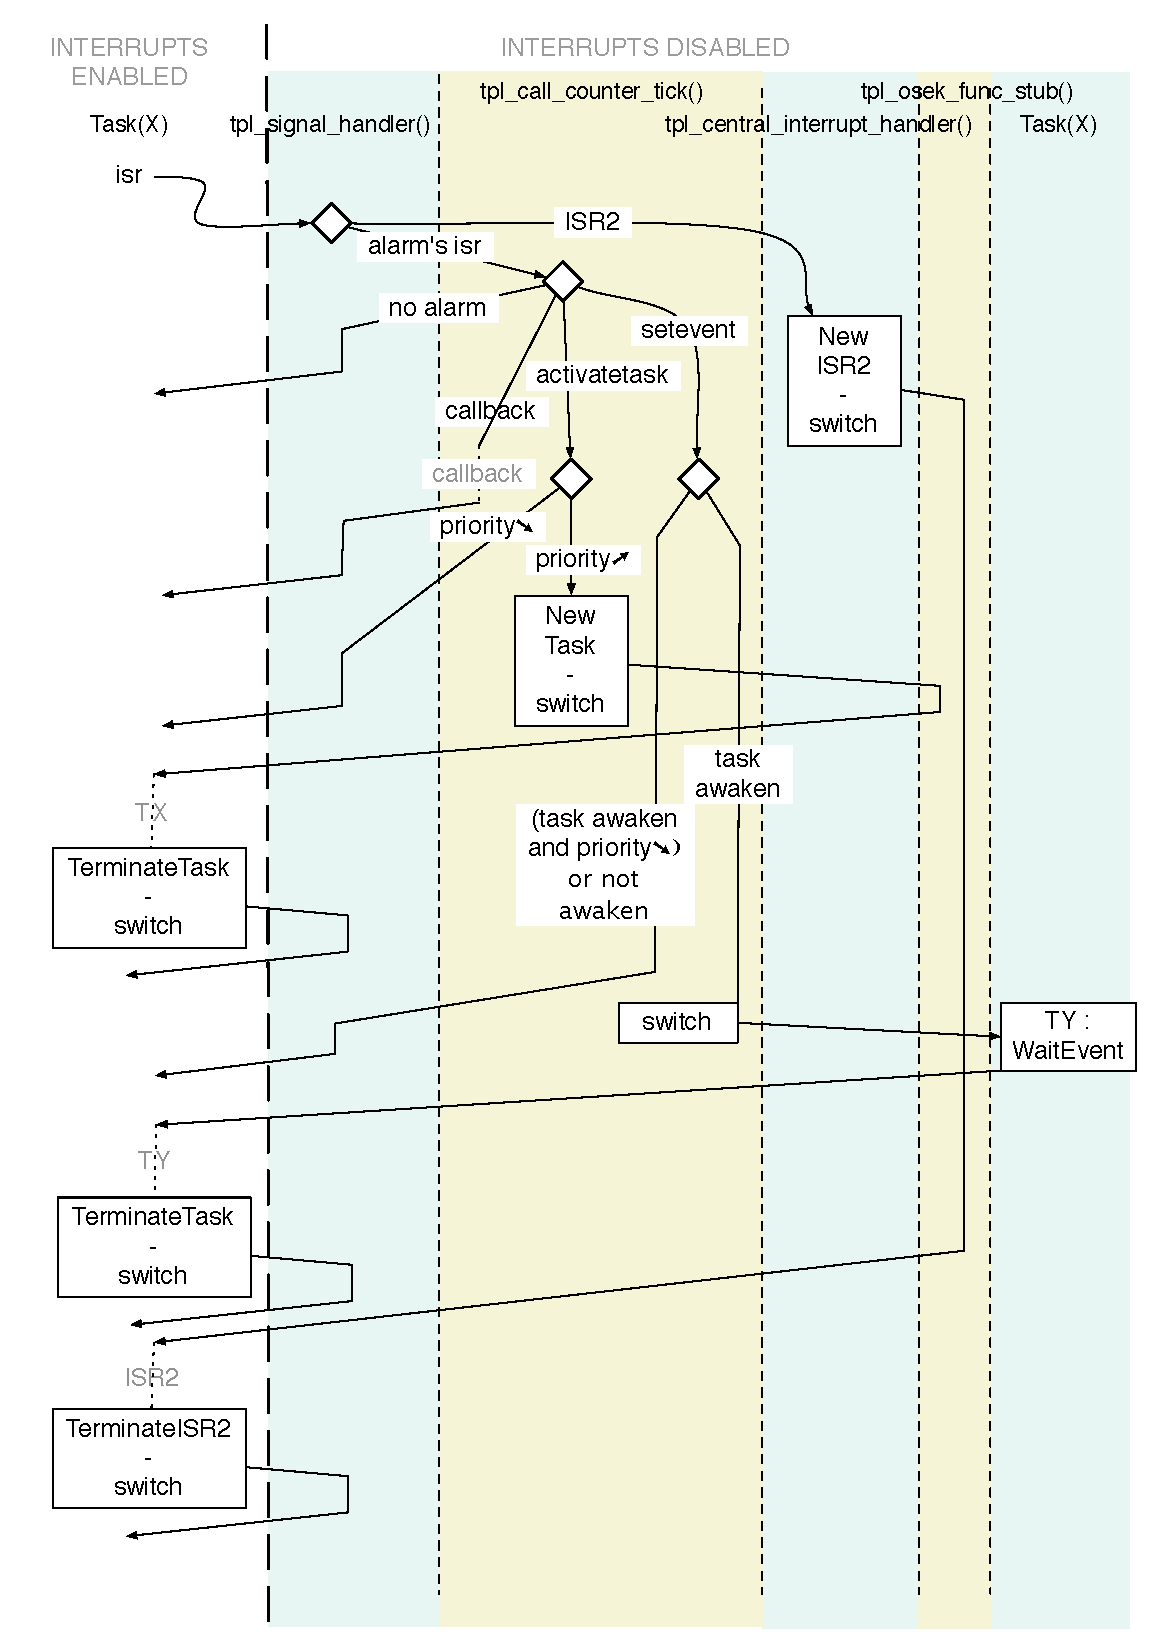
\includegraphics[width=0.8\textwidth]{graphics/Interrupts_Management.pdf}
	\end{figure}
	
\bibliographystyle{plain} 
\bibliography{Bib} 

\end{document}